\chapter{Sistema proposto}

Lo scopo di questo capitolo è quello di fornire una soluzione progettuale al problema mostrato nel capitolo precedente. Verranno quindi trattate le problematiche affrontate durante la fase di trasformazione del progetto in un artefatto eseguibile ed infine offerta una valutazione complessiva del sistema prodotto, illustrando preventivamente le informazioni relative alle metriche di valutazione utilizzate e alla natura dei test condotti.

\section{Architettura}

\begin{figure}[h]
\centering
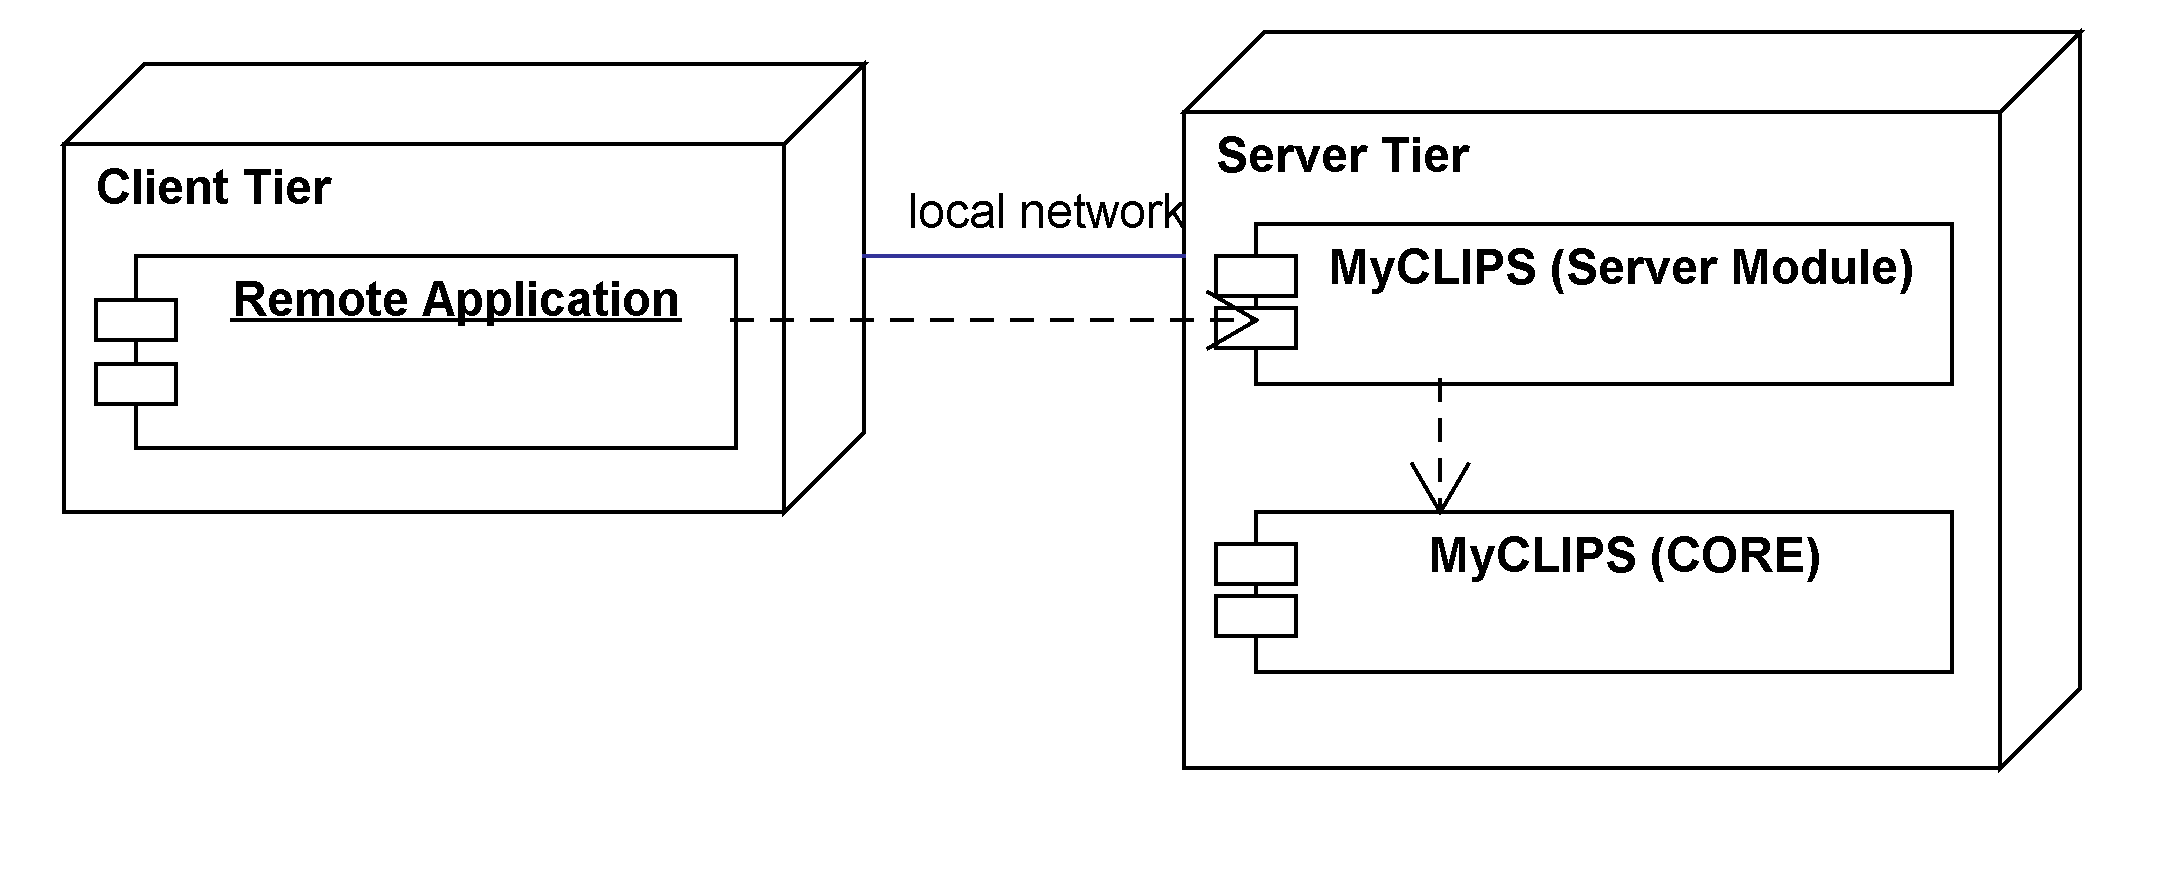
\includegraphics[width=0.8\textwidth]{Immagini/Capitolo3/Deployment/Client-Server.png}
\caption[Vista generale dell'architettura di sistema]{Vista generale dell'architettura di sistema: i servizi offerti dal modulo principale vengono distribuiti ad una serie di applicazioni remote attraverso l'utilizzo del componente Server}\label{fig:architettura-client-server}
\end{figure}

Il sistema proposto è composto da due componenti principali distinte. Una prima, il \emph{core} del sistema MyCLIPS, realizza i servizi previsti dall'environment in una serie di API. Una seconda, il \emph{modulo server}, si pone come tramite fra i servizi offerti dalla prima componente e un gruppo di client, distribuendo le caratteristiche attraverso un modello d'architettura \emph{Client-Server}~(\figurename~\ref{fig:architettura-client-server}).

\begin{figure}[h]
\centering
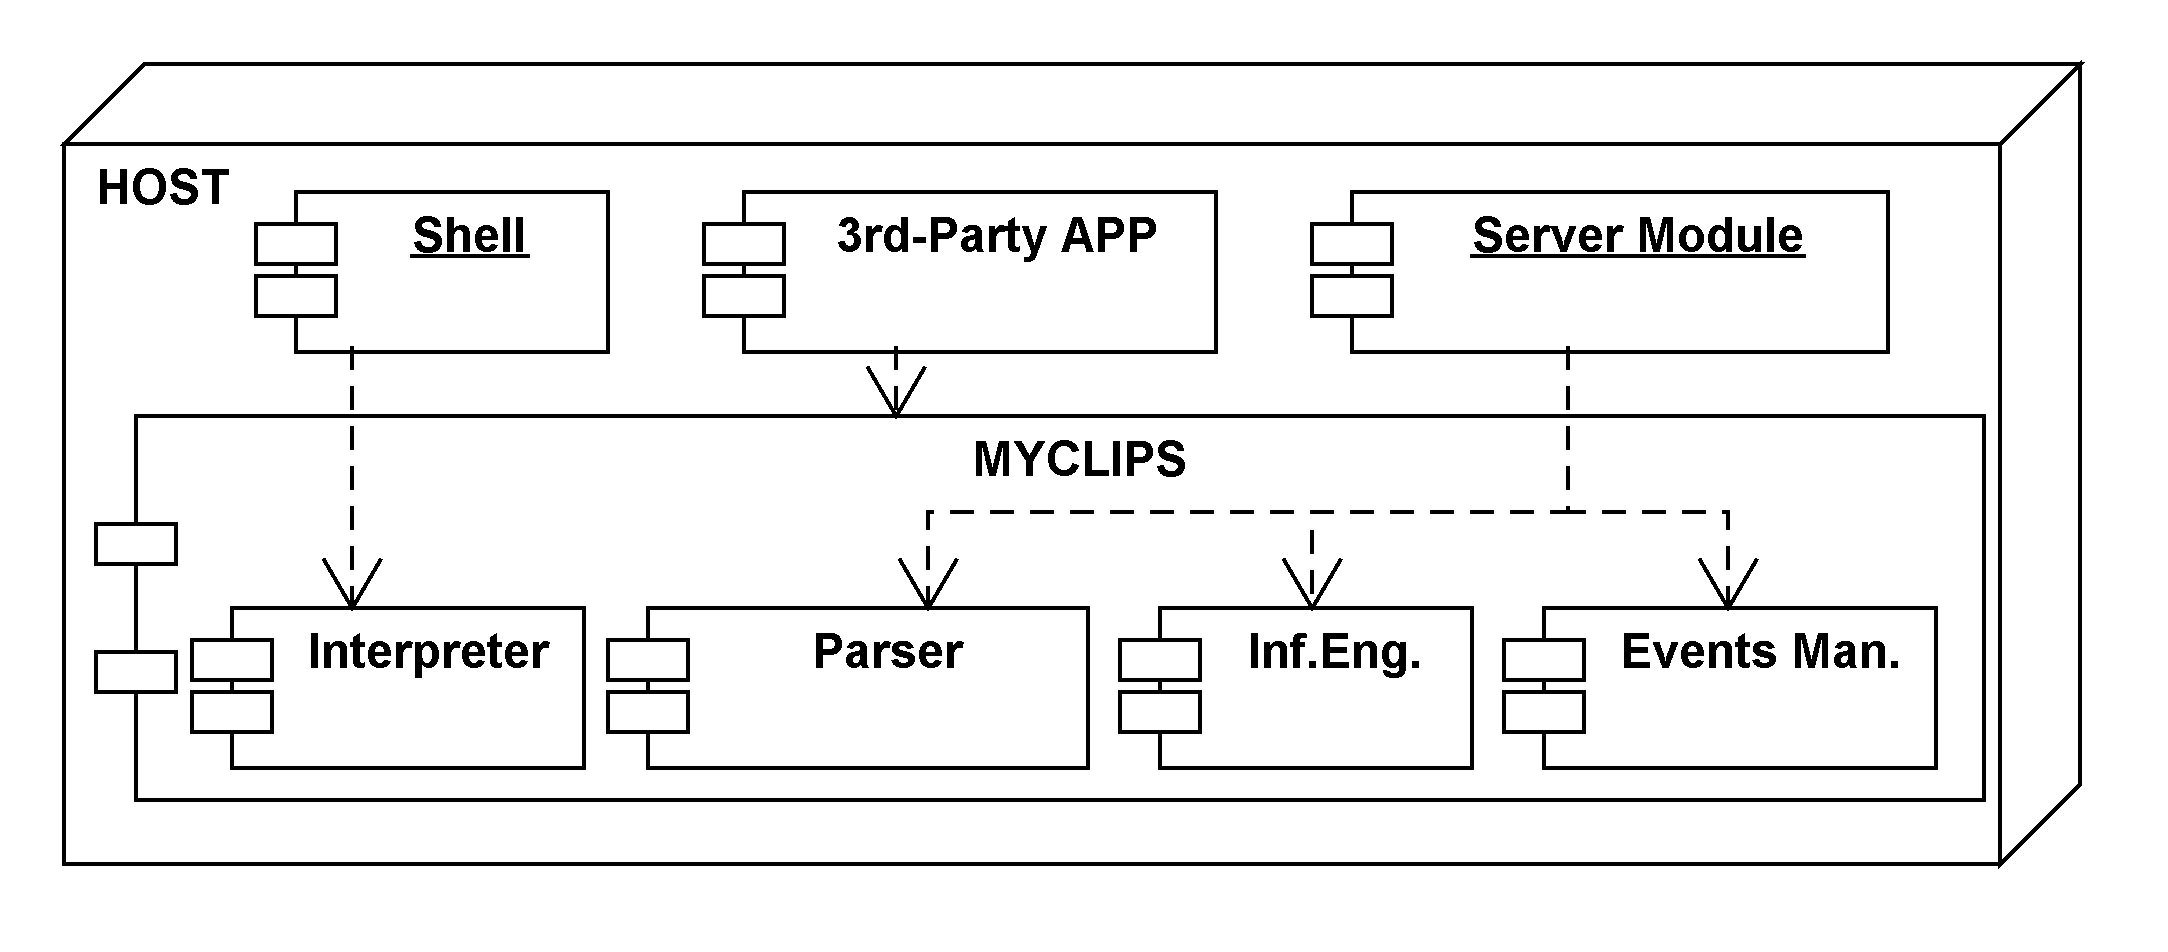
\includegraphics[width=0.9\textwidth]{Immagini/Capitolo3/Deployment/Shell-3rdPartyApp.png}
\caption[Vista generale dell'architettura locale di sistema]{Vista generale dell'architettura locale di sistema: i componenti del \emph{core} vengono utilizzati da componenti esterne (\emph{shell}, \emph{modulo server} o applicazioni generiche)}\label{fig:architettura-3rdparty}
\end{figure}

Il \emph{modulo server} è sia un elemento di sistema, che un esempio d'istanza di applicazione generica che utilizza i servizi offerti dal \emph{core}. Un altro esempio è quello del componente \emph{shell}: un elemento distinto che utilizza le interfacce del \emph{core} per realizzare un terminale testuale con il quale utilizzare l'\emph{environment}~(\figurename~\ref{fig:architettura-3rdparty}).


\subsection{Core}

La componente principale è quella rappresentata dal \emph{core} di MyCLIPS: racchiude tutti i \emph{package} necessari alla realizzazione dei servizi principali del sistema~(\figurename~\ref{fig:packages-myclips}).

\begin{figure}[h]
\centering
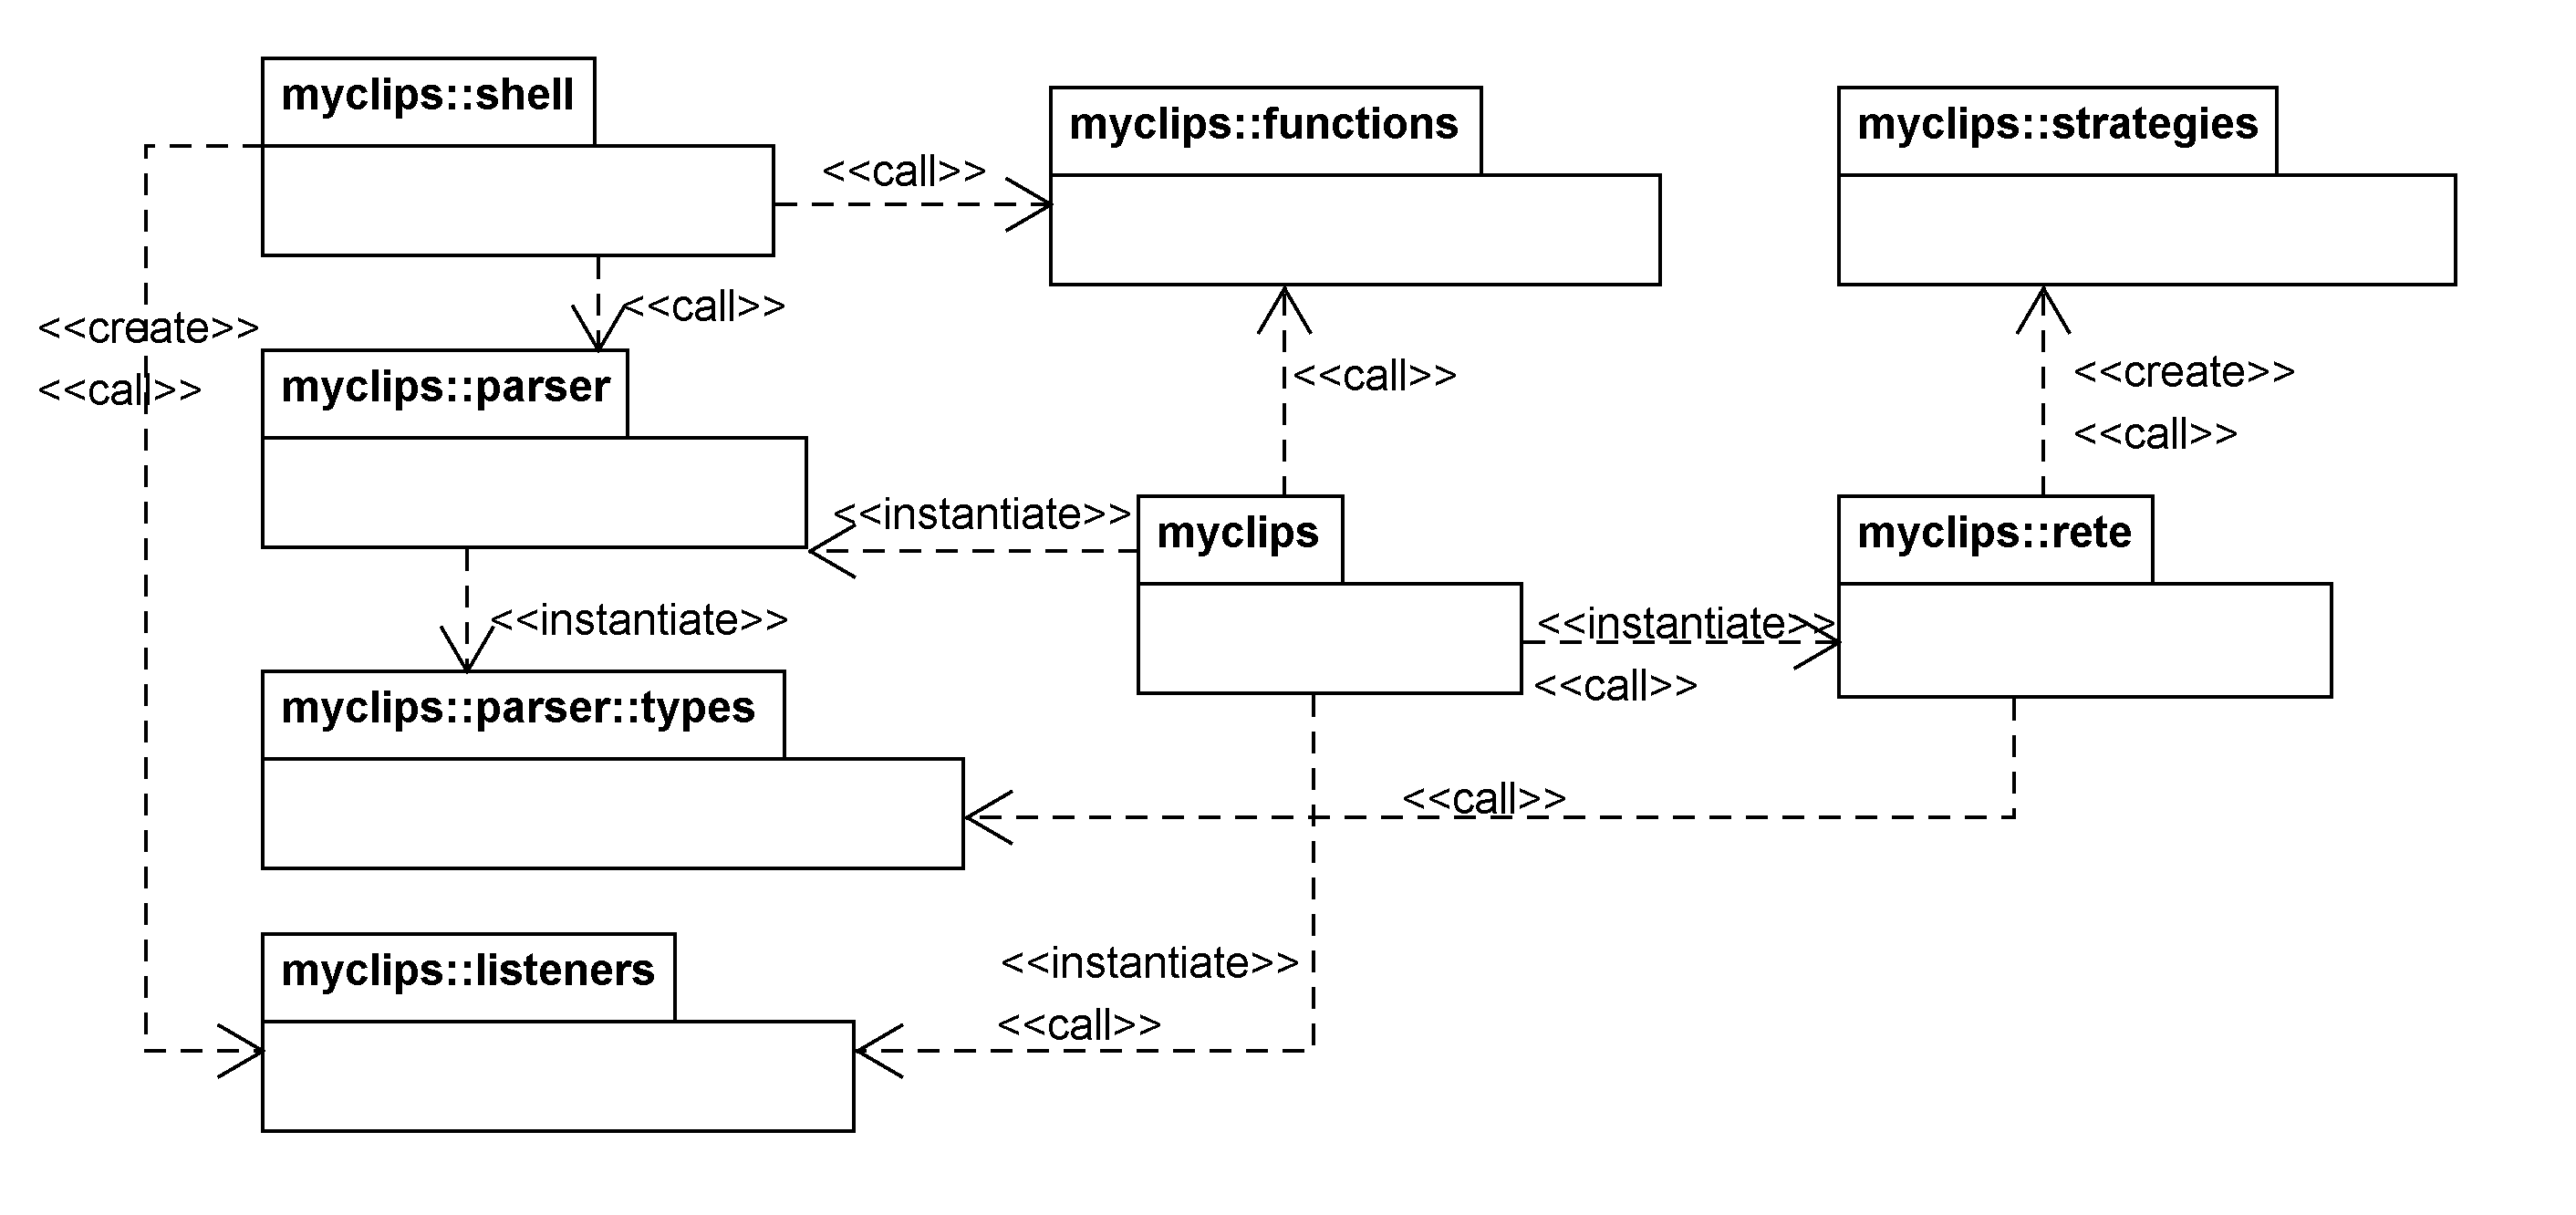
\includegraphics[width=1\textwidth]{Immagini/Capitolo3/Packages/Core.png}
\caption{Package \emph{myclips}: vista dei \emph{package} che compongono il \emph{core}}\label{fig:packages-myclips}
\end{figure}

Lo scopo dei singoli \emph{package}, con riferimento alle funzionalità che realizzano, è dettagliato nel proseguo dei paragrafi.

\subsubsection{Modulo Parser}

\begin{figure}[h]
\centering
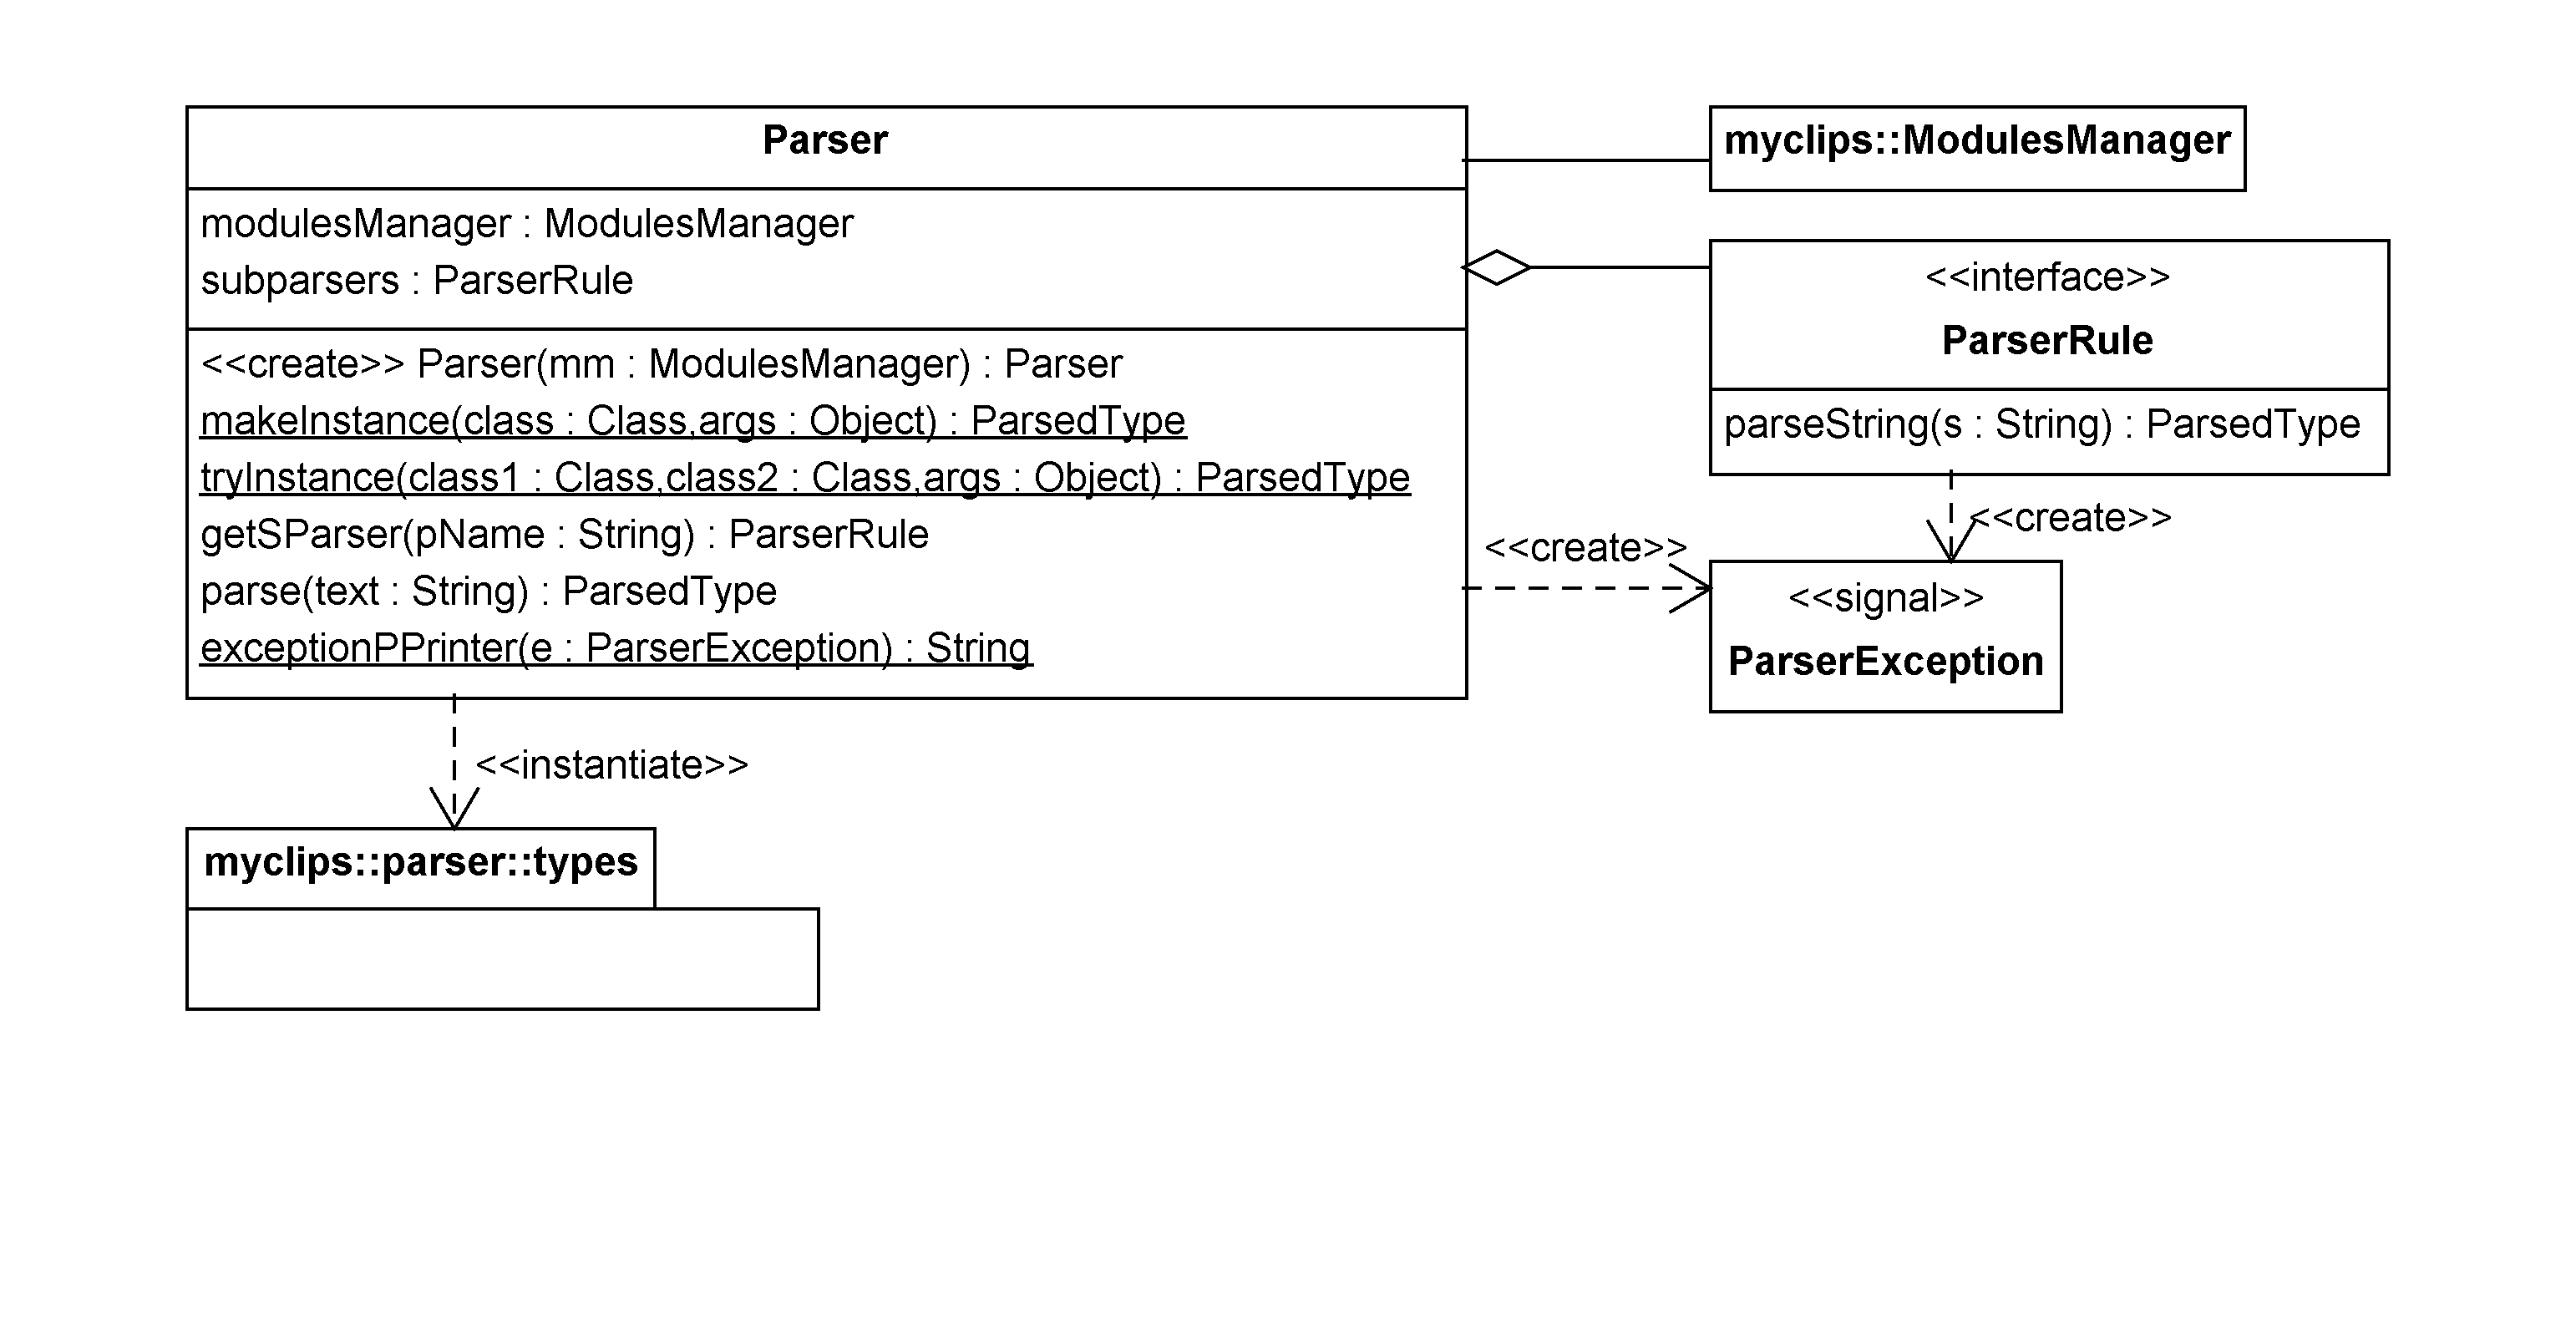
\includegraphics[width=1\textwidth]{Immagini/Capitolo3/Classi/myclips_parser_Parser.png}
\caption{Package \emph{myclips.parser}: vista delle classi relative al \emph{Parser}}\label{fig:class-myclips-parser-Parser}
\end{figure}

Il \emph{package} \emph{Parser} comprende l'insieme di classi e interfacce che realizzano la funzionalità di analisi e conversione del linguaggio di specifica in istanze utilizzabili dal motore inferenziale per il compimento delle proprie attività.

L'elemento principale del \emph{package} è la classe \emph{Parser}~(\figurename~\ref{fig:class-myclips-parser-Parser}), che organizza le regole di conversione (rappresentate dall'interfaccia \emph{ParserRule}) ed effettua le operazioni di conversione del testo in istanze. Le classi utilizzate per la rappresentazione dei costrutti convertiti sono organizzate all'interno del \emph{sub-package} \emph{myclips.parser.types}.

Il \emph{sub-package} contiene l'insieme di classi relative alla rappresentazione dei tipi atomici di base e dei costrutti compositi.

\begin{figure}[h]
\centering
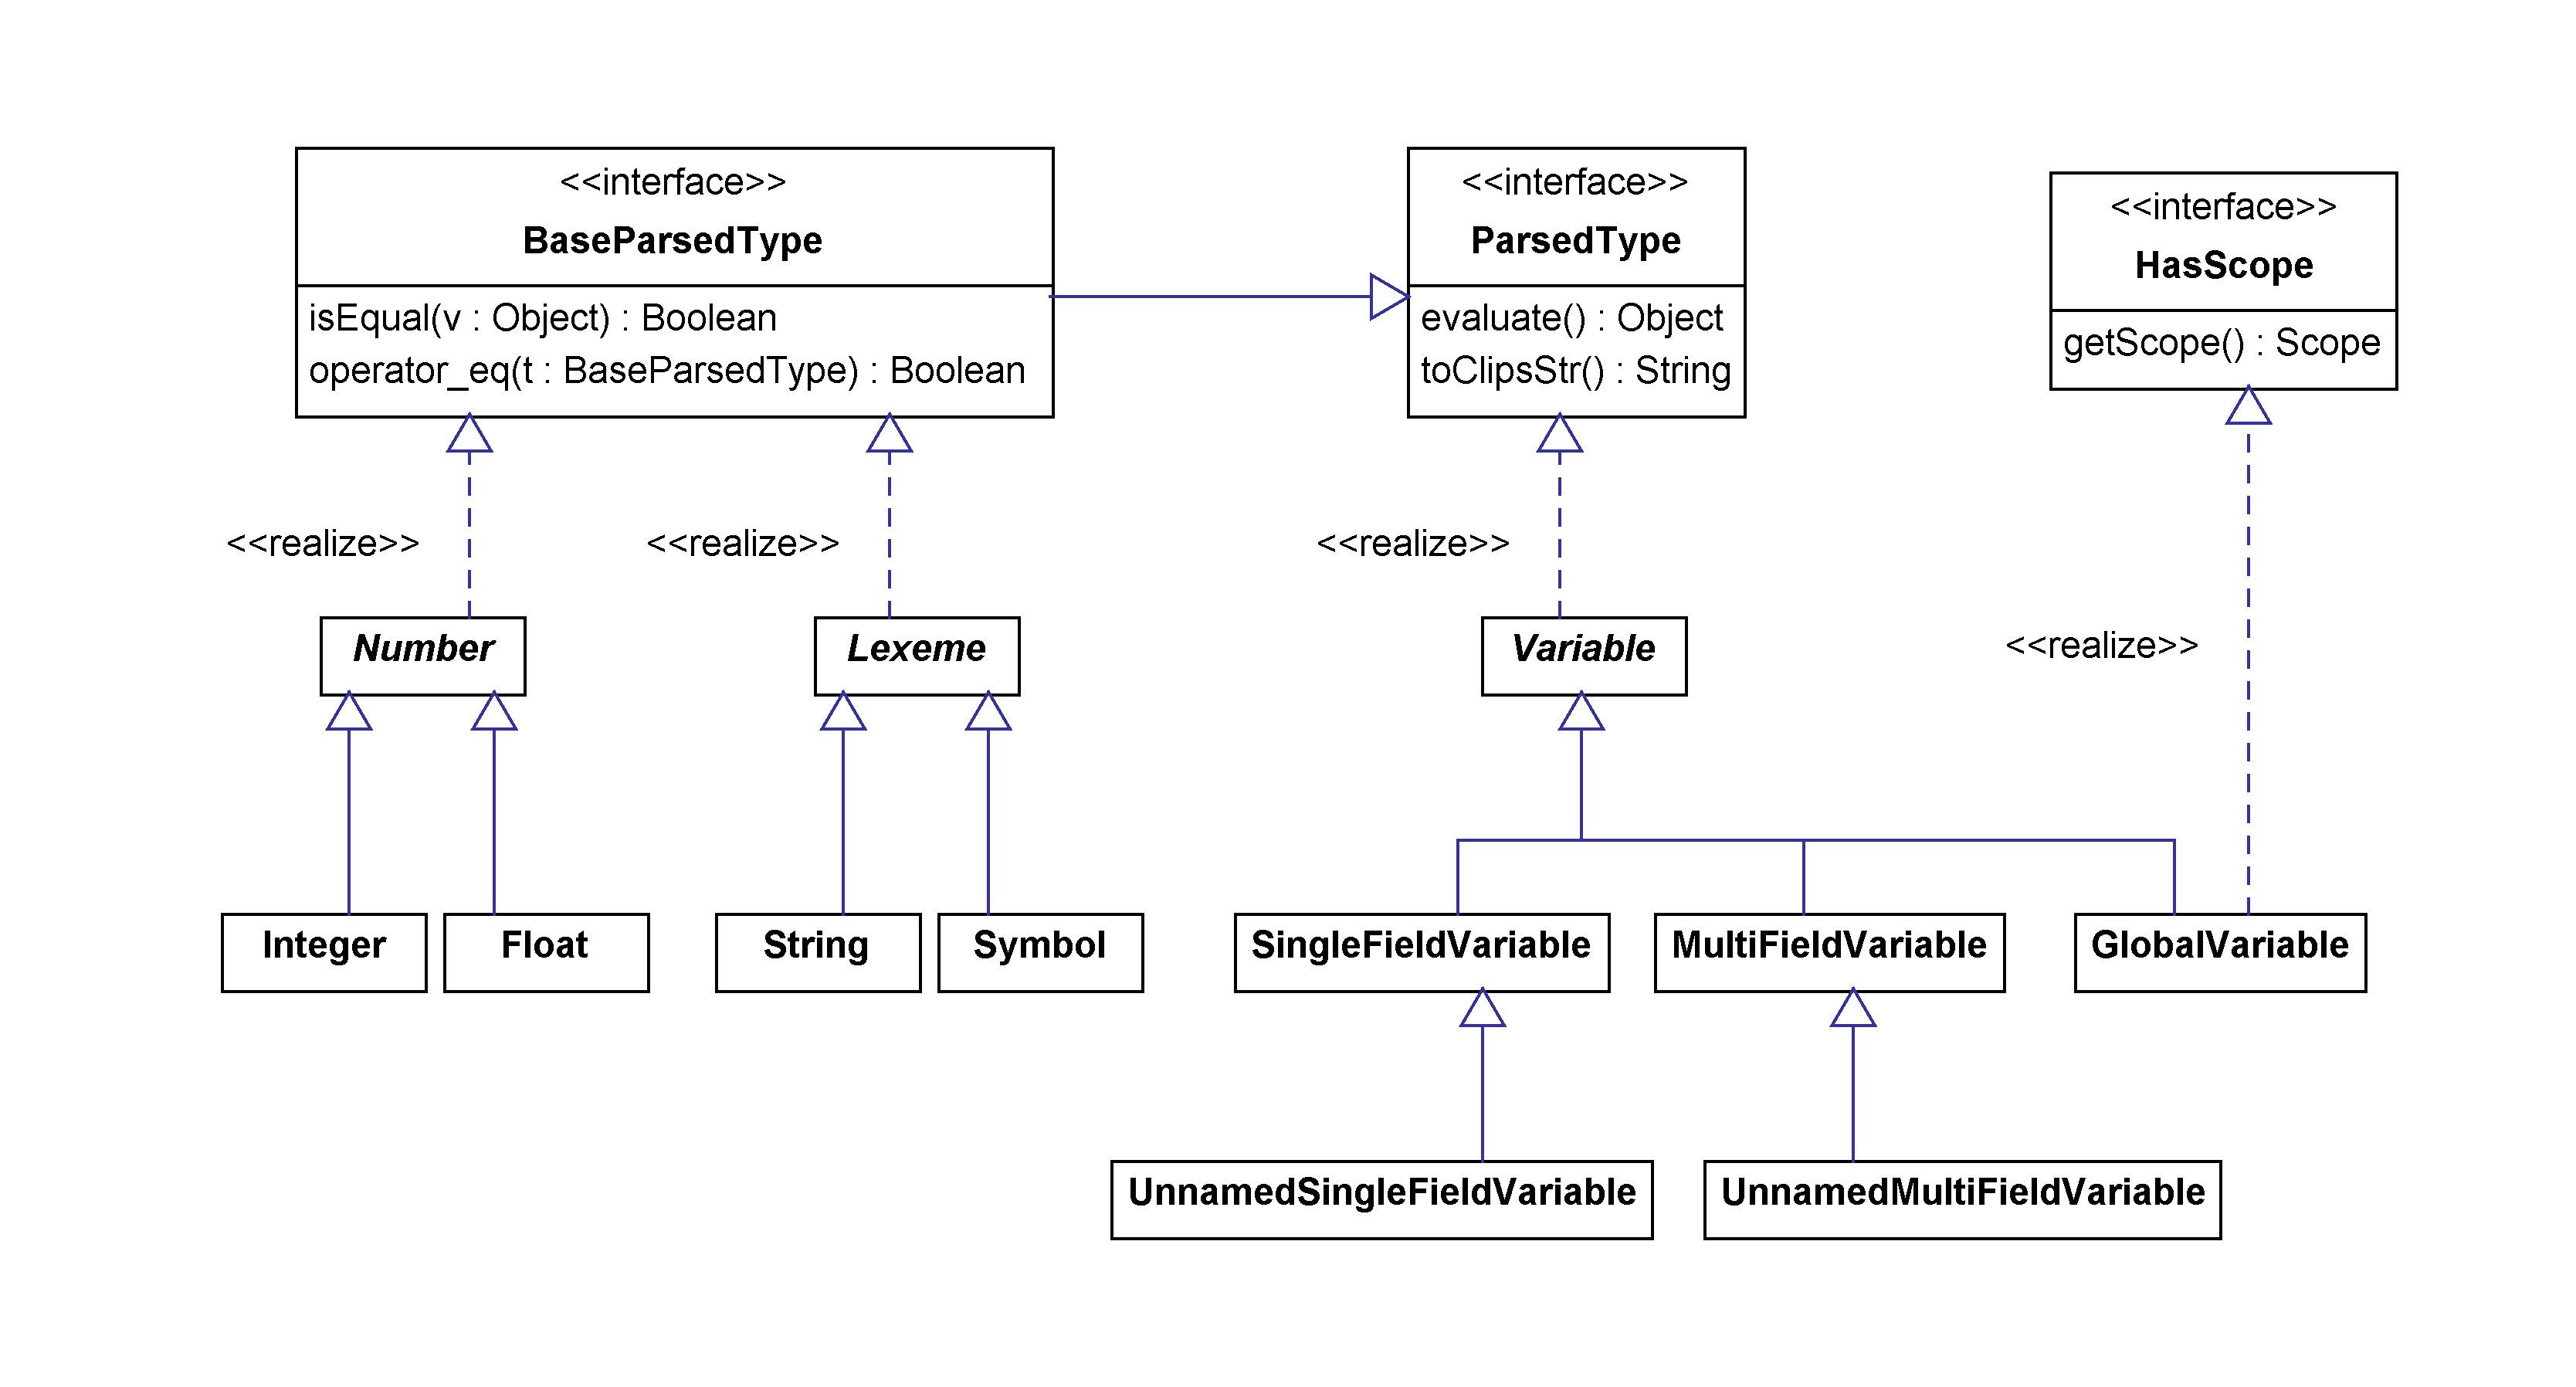
\includegraphics[width=0.8\textwidth]{Immagini/Capitolo3/Classi/myclips_parser_types_Atoms.png}
\caption{Package \emph{myclips.parser.types}: vista di classi e interfacce per gli elementi atomici}\label{fig:class-myclips-parser-types-Atoms}
\end{figure}

La gerarchia di tipi atomici supportata dal sistema segue le specifiche relative ai tipi proposti da CLIPS. Fanno parte di questa classificazione \emph{Lexeme}, specializzato da \emph{Symbol} e \emph{String}, e \emph{Number}, specializzato da \emph{Integer} e \emph{Float}. A questi tipi si uniscono quelli per la rappresentazioni delle variabili~(\figurename~\ref{fig:class-myclips-parser-types-Atoms}).

\begin{figure}[h]
\centering
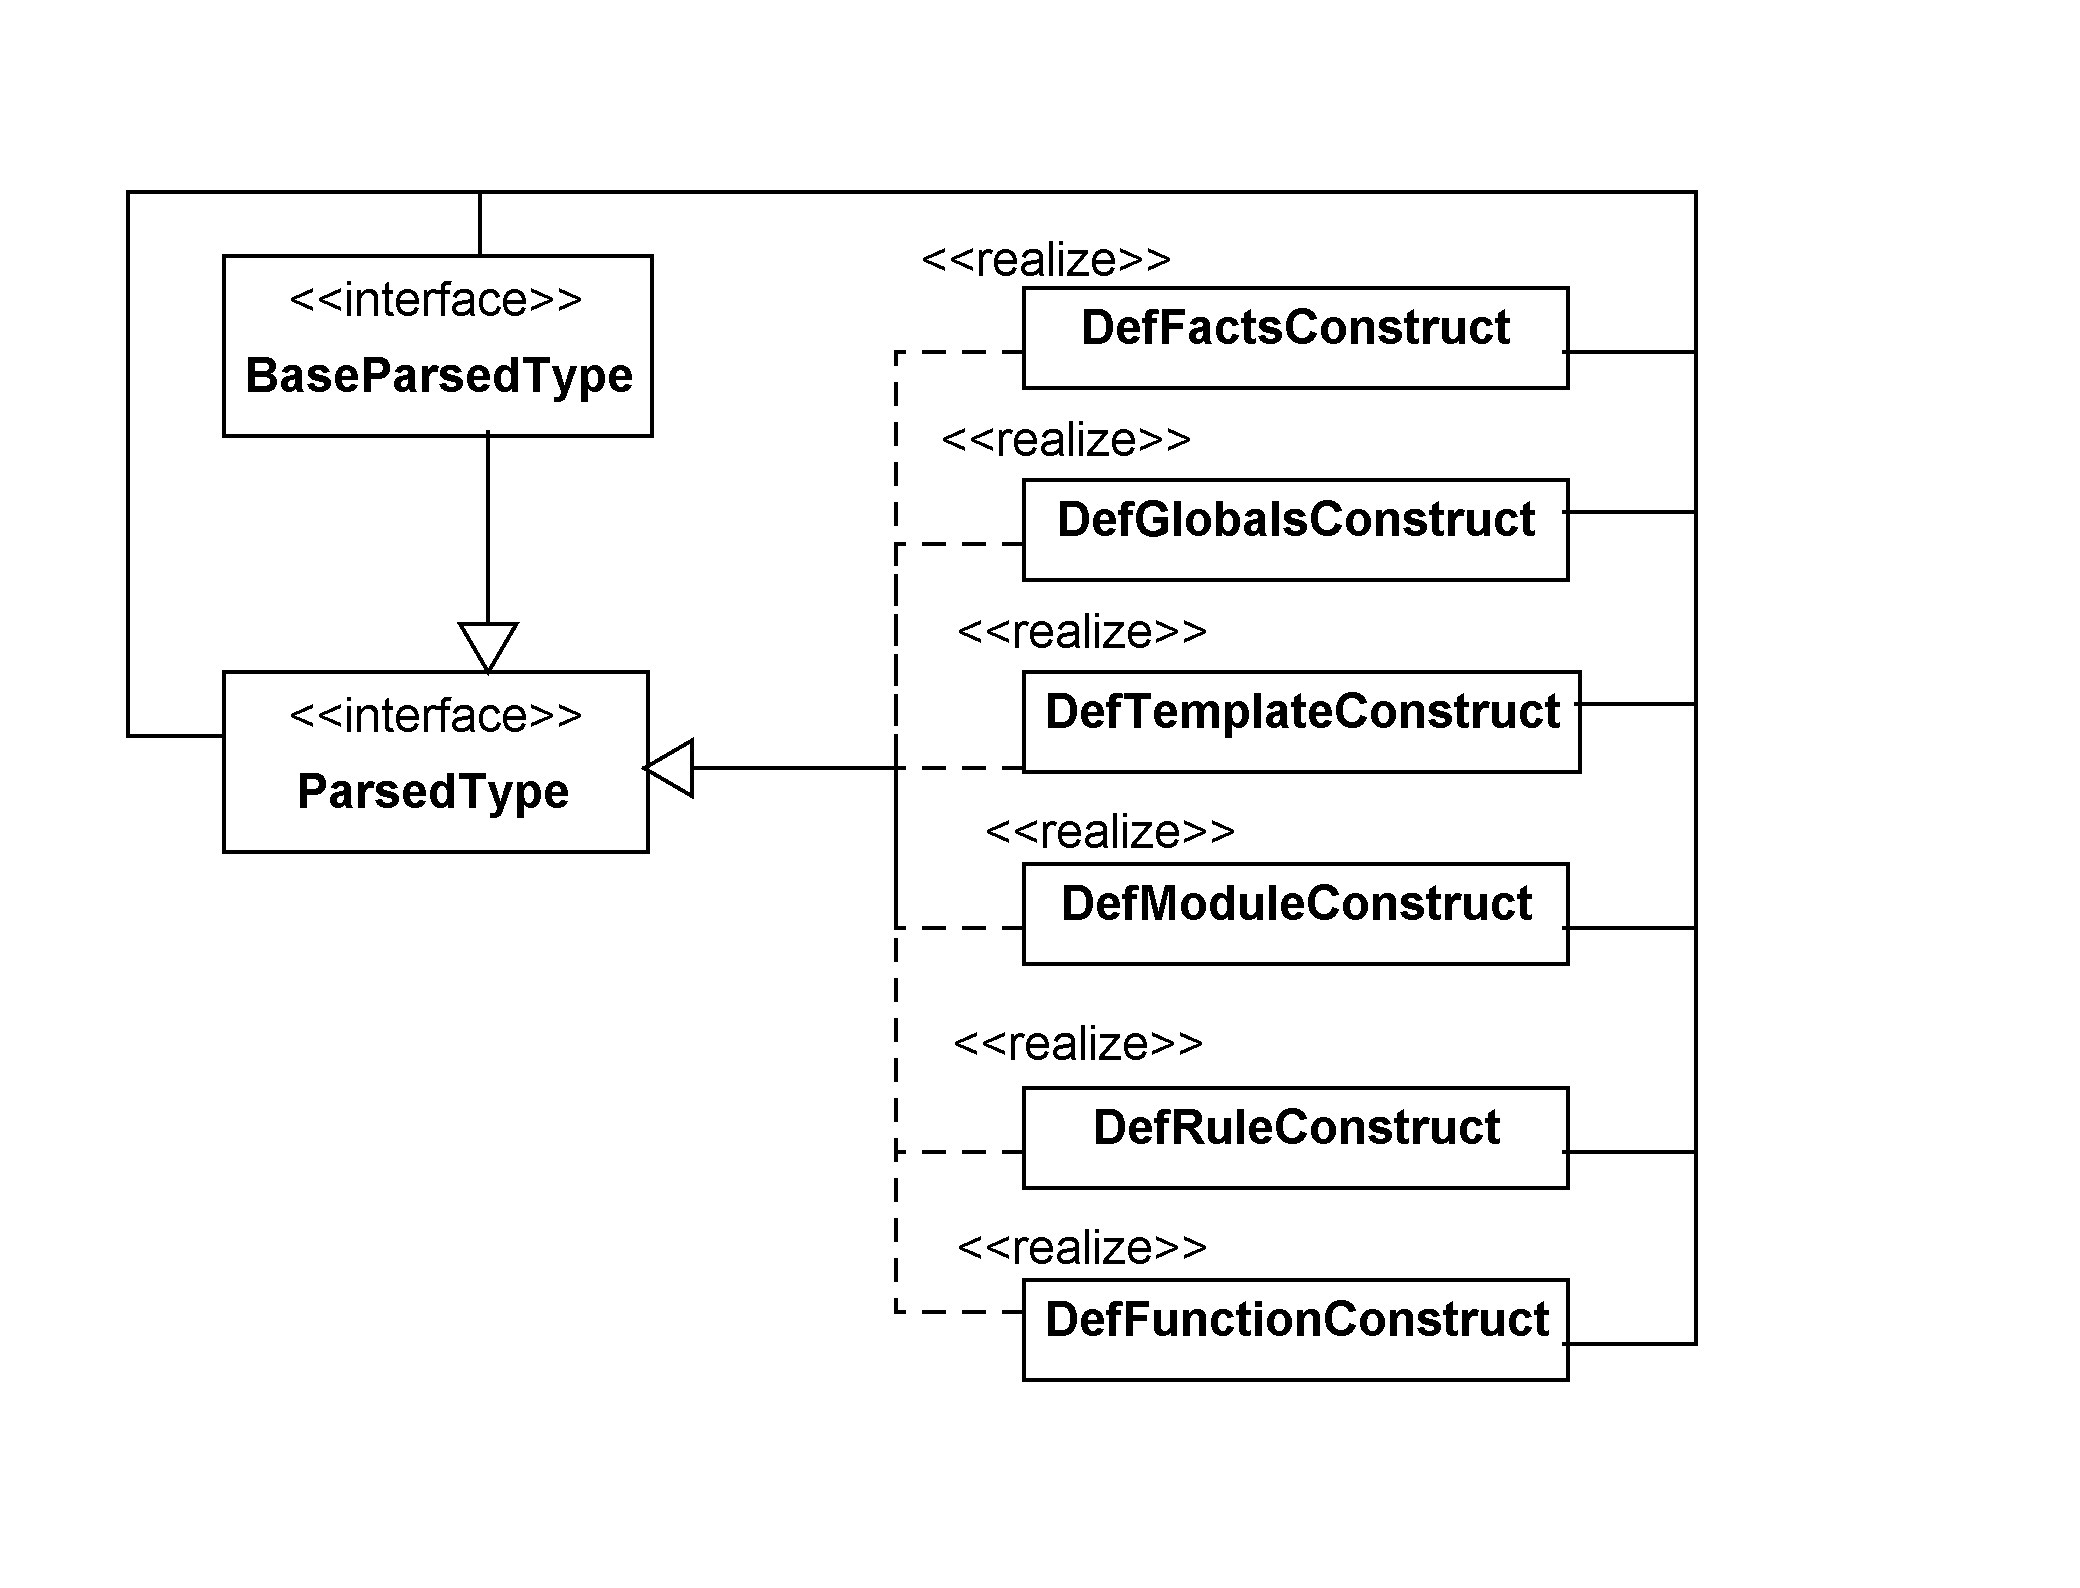
\includegraphics[width=0.8\textwidth]{Immagini/Capitolo3/Classi/myclips_parser_types_Constructs.png}
\caption{Package \emph{myclips.parser.types}: vista di classi e interfacce per i costrutti principali}\label{fig:class-myclips-parser-types-Constructs}
\end{figure}

La composizione dei tipi di base realizza un insieme di costrutti complessi principali. Le classi mostrate in \figurename~\ref{fig:class-myclips-parser-types-Constructs} sono le rappresentazioni corrispondenti ai formalismi \emph{defrule}, \emph{defglobals}, \emph{deffunction}, \emph{deftemplate} e \emph{defmodule}, utilizzate dal linguaggio di specifica per la formalizzazione dei sistemi esperti.

\begin{figure}[h]
\centering
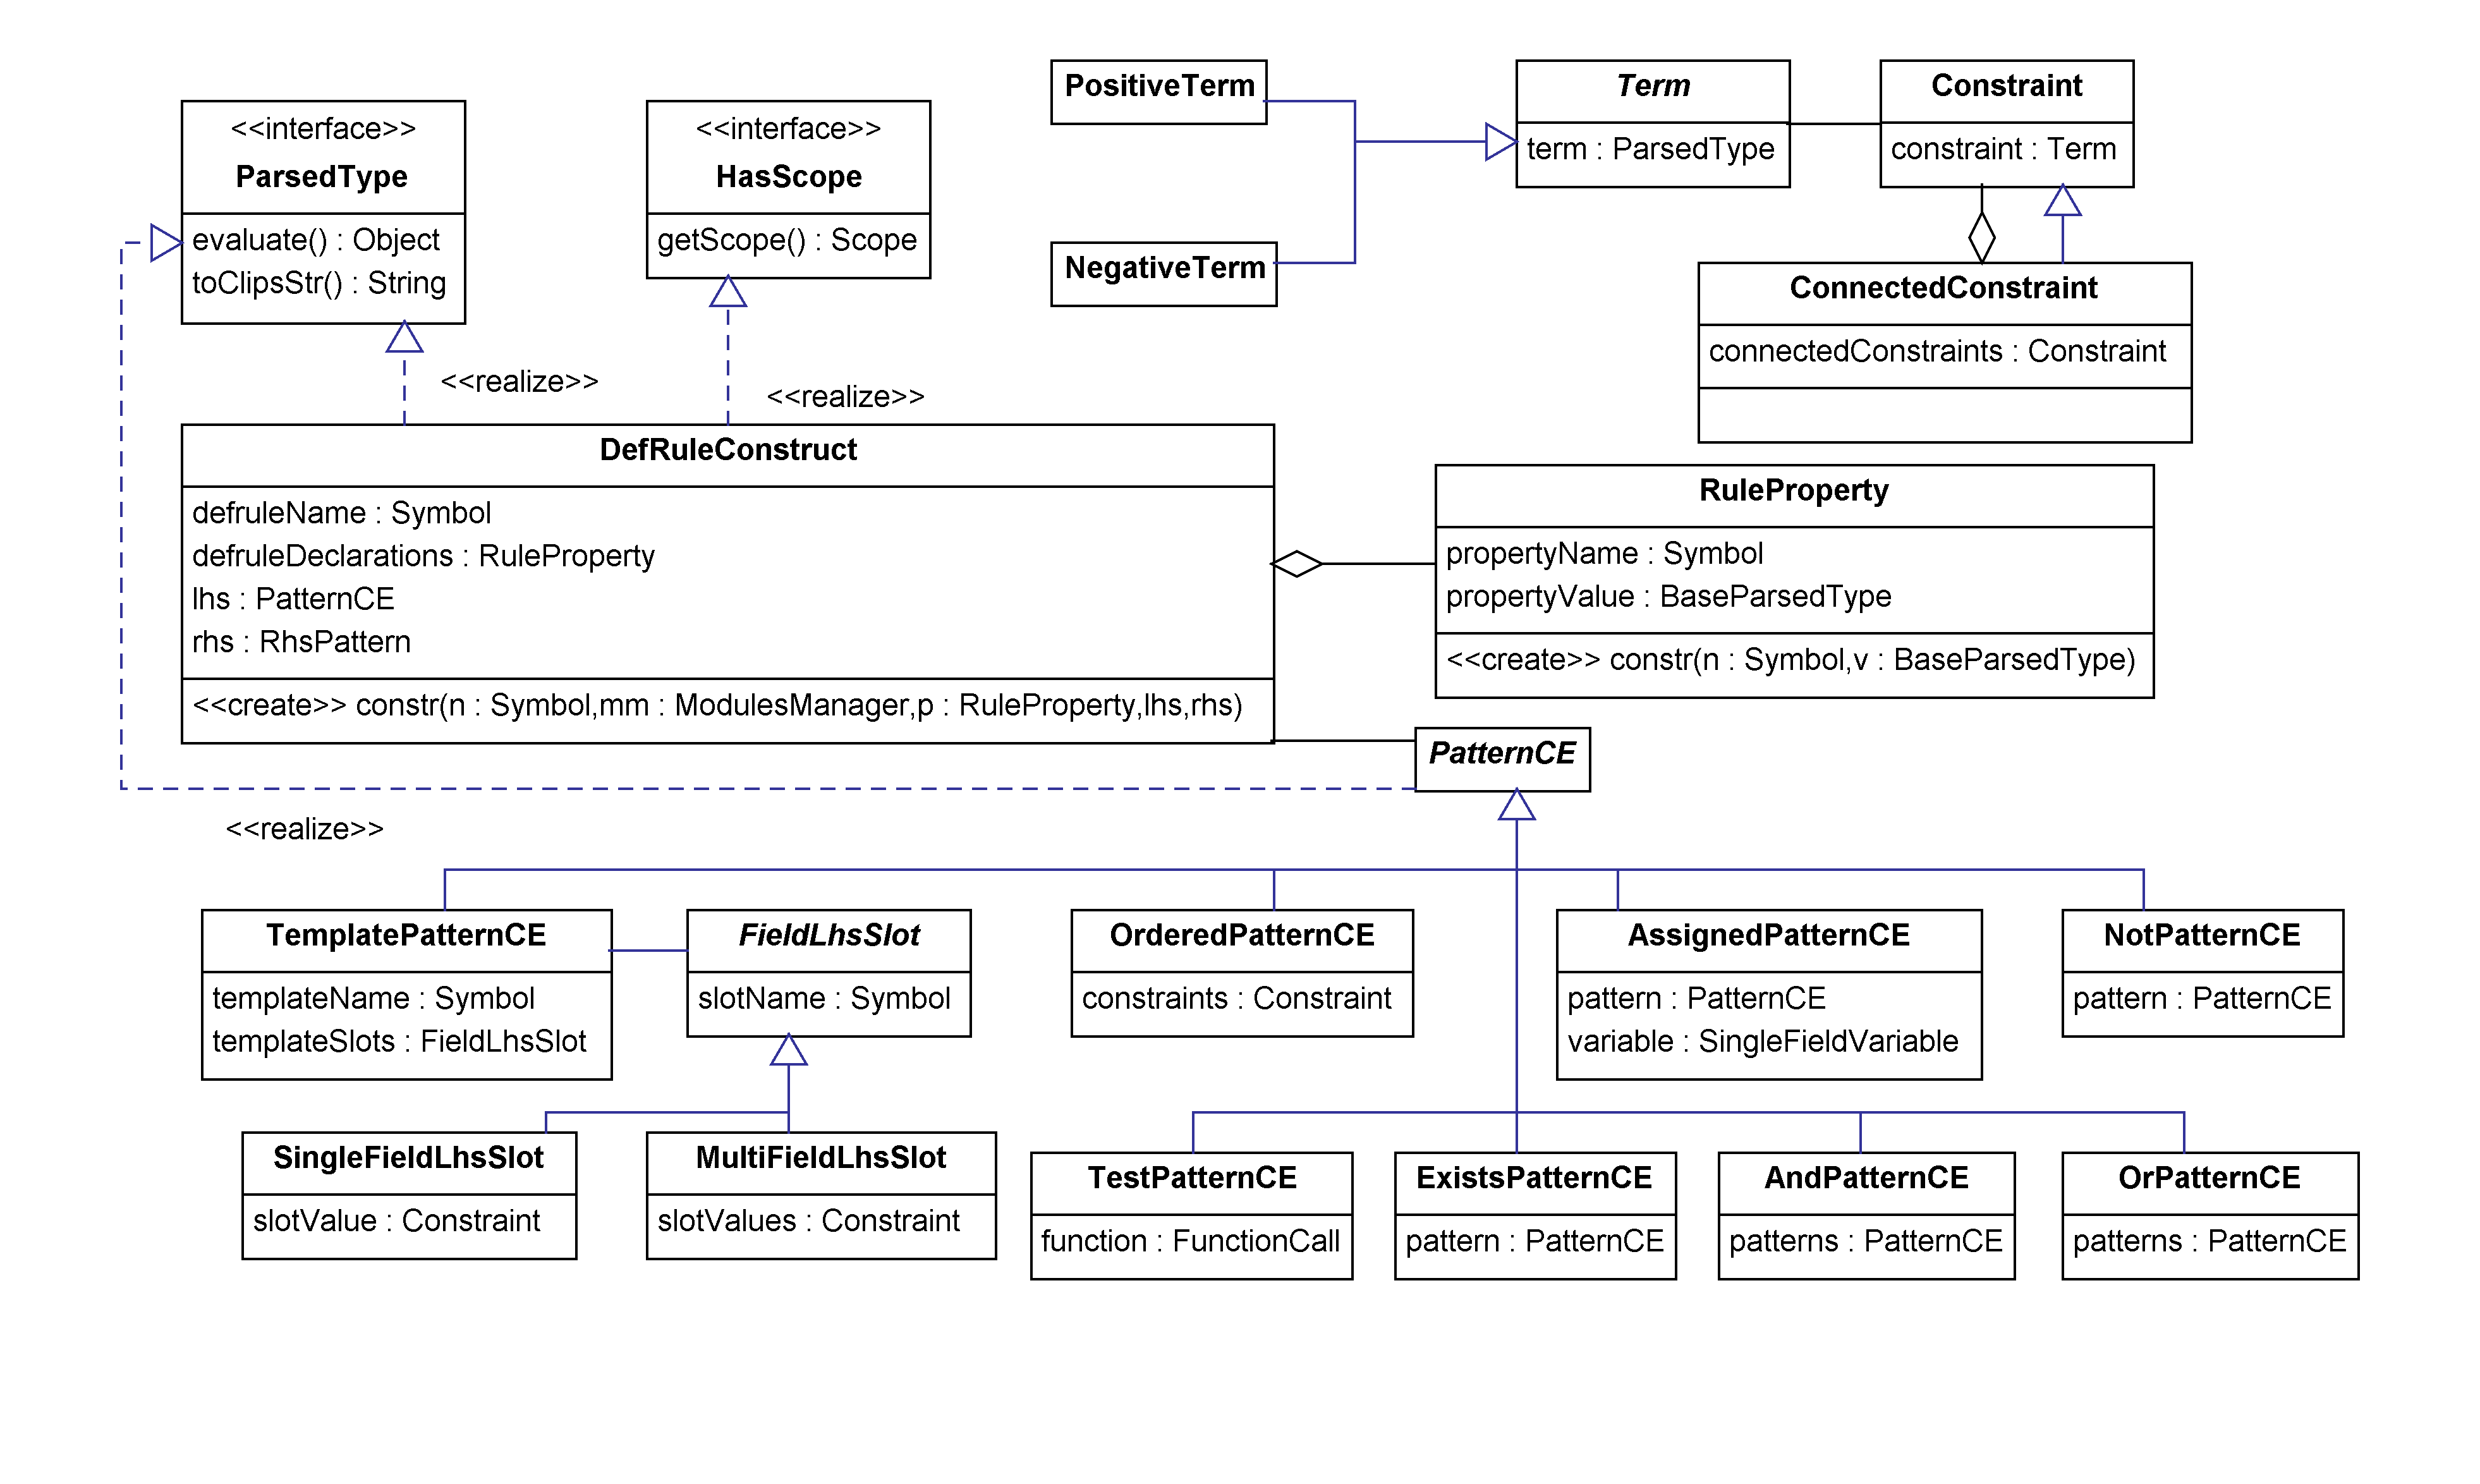
\includegraphics[width=1\textwidth]{Immagini/Capitolo3/Classi/myclips_parser_types_DefRule.png}
\caption{Package \emph{myclips.parser.types}: vista delle classi e interfacce relative al costrutto \emph{defrule}}\label{fig:class-myclips-parser-types-DefRuleConstruct}
\end{figure}

%\begin{figure}[h]
%\centering
%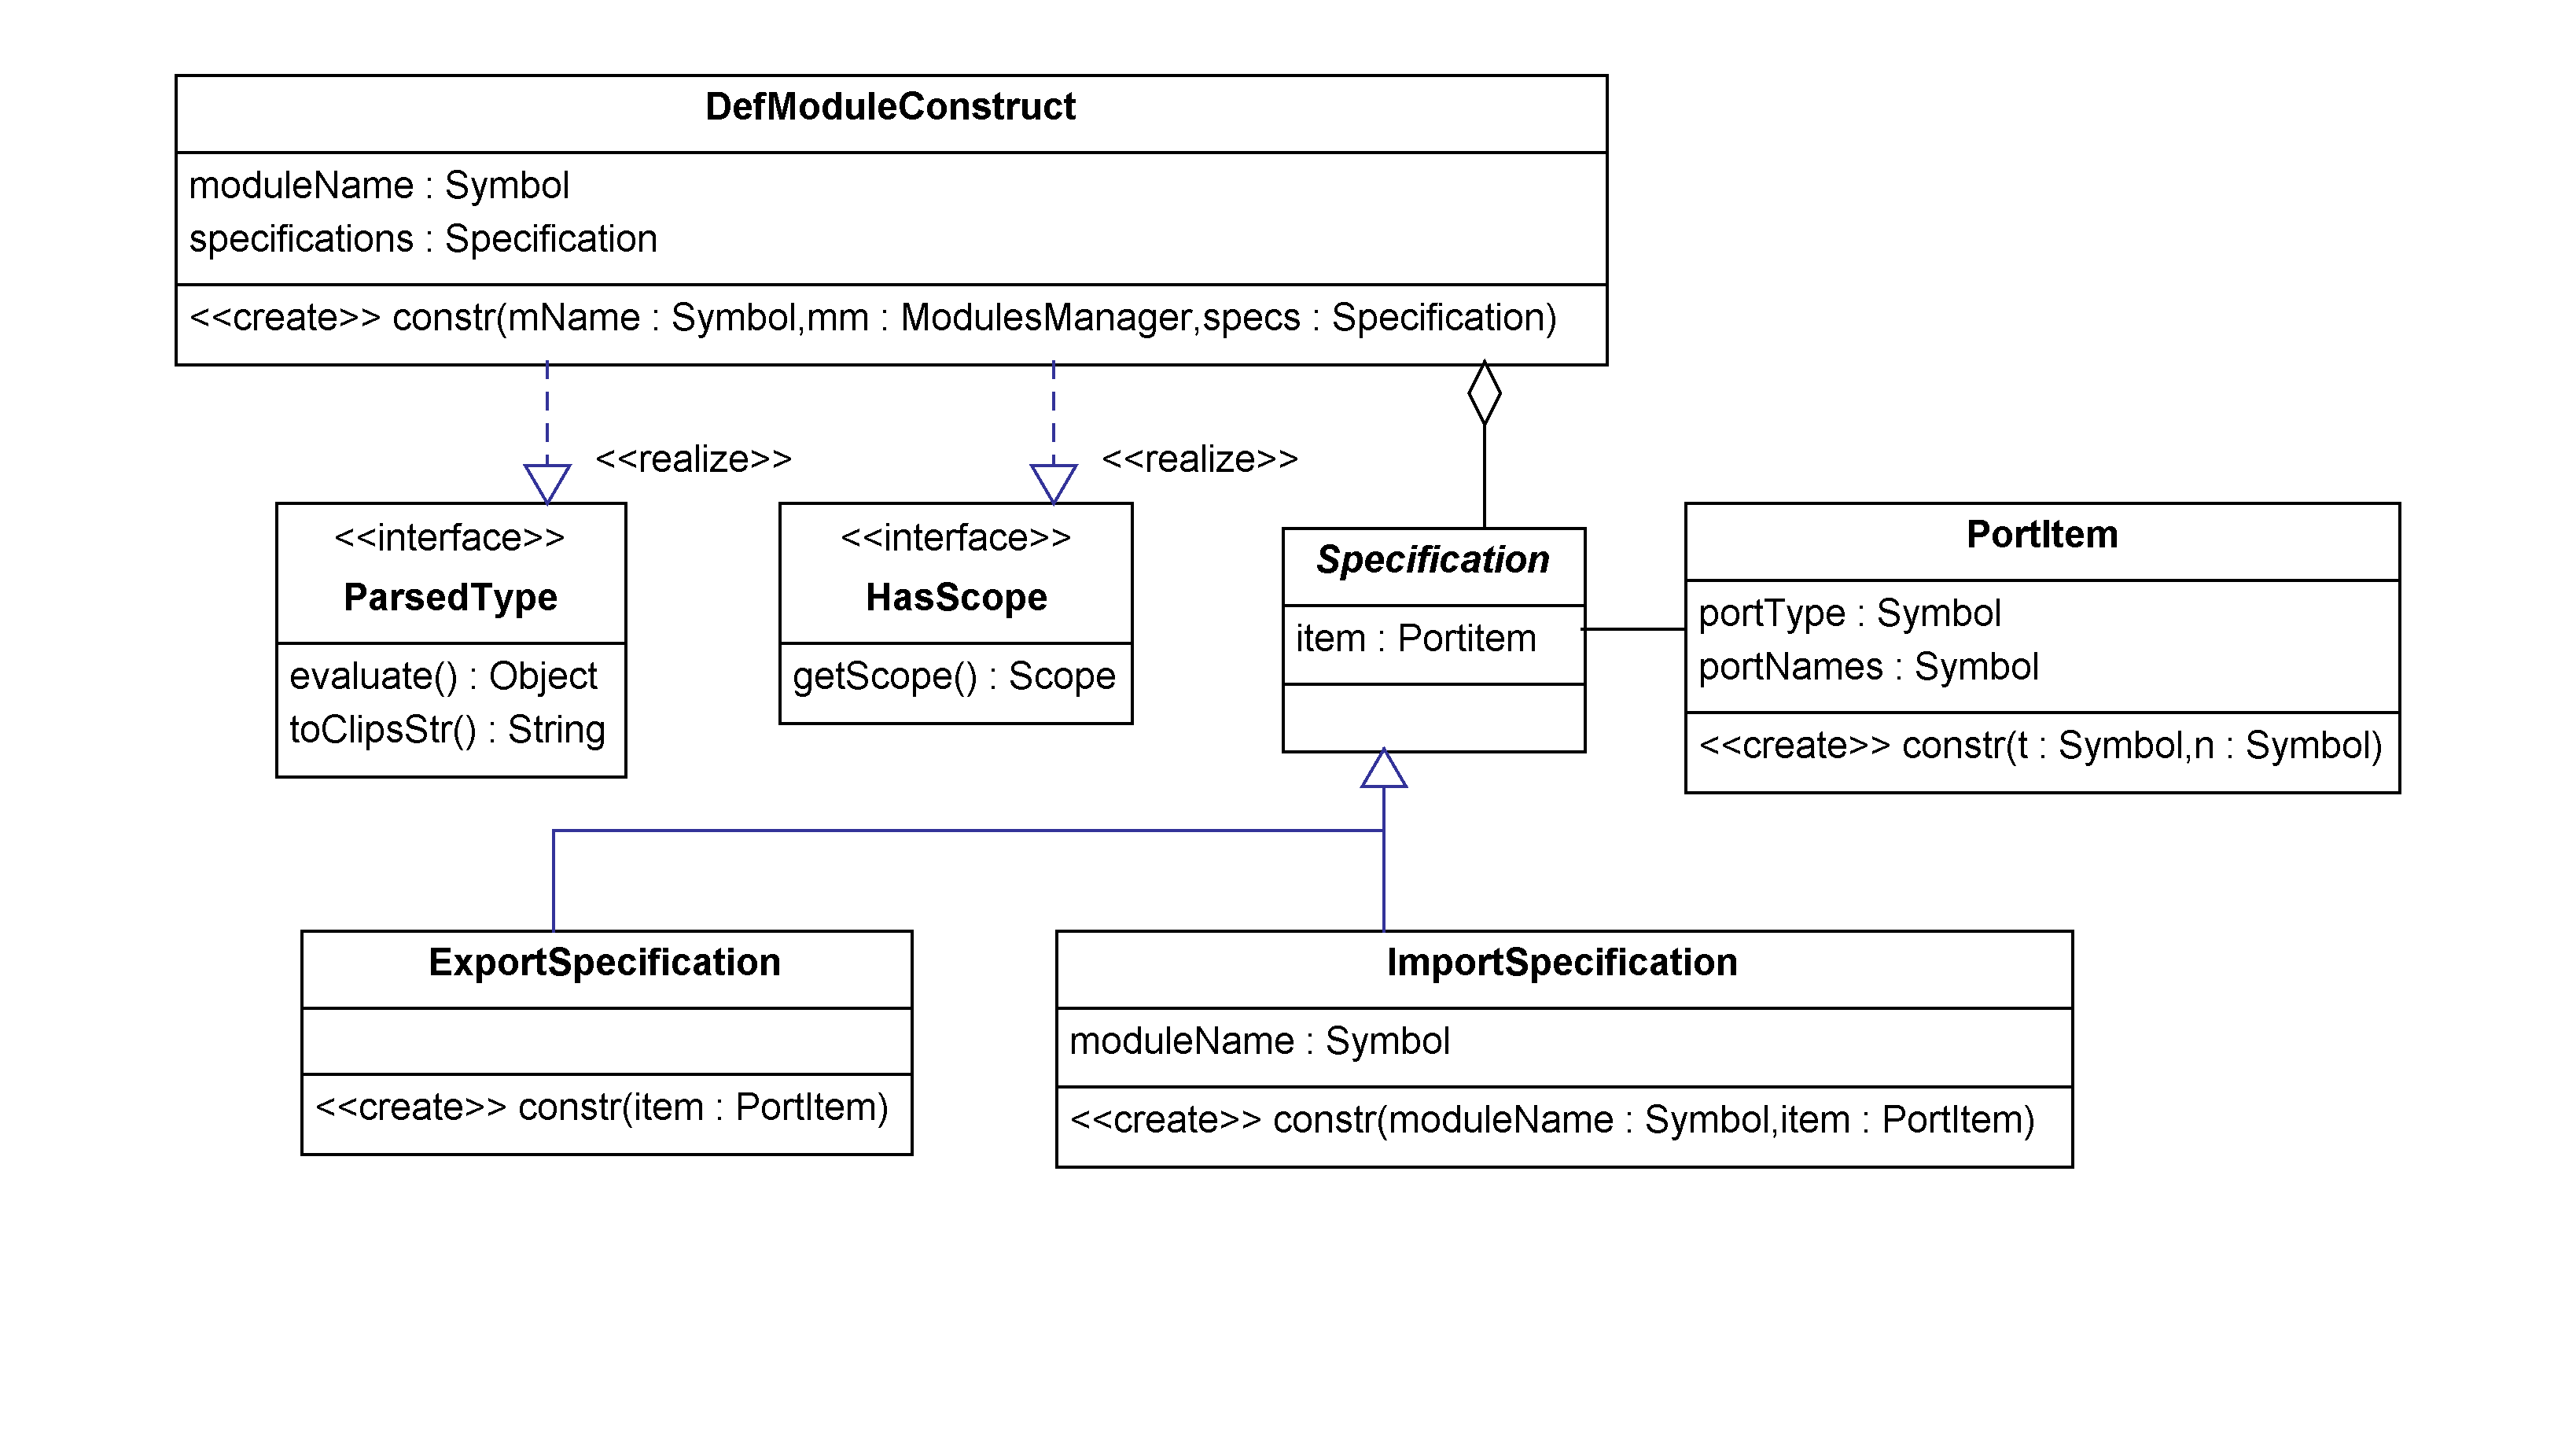
\includegraphics[width=0.9\textwidth]{Immagini/Capitolo3/Classi/myclips_parser_types_DefModule.png}
%\caption{Package \emph{myclips.parser.types}: vista delle classi e interfacce relative al costrutto \emph{defmodule}}\label{fig:class-myclips-parser-types-DefModuleConstruct}
%\end{figure}


%A titolo d'esempio di propongono le strutture delle classi \emph{DefRuleConstruct}~(\figurename~\ref{fig:class-myclips-parser-types-DefRuleConstruct}) e \emph{DefModuleConstruct}~(\figurename~\ref{fig:class-myclips-parser-types-DefModuleConstruct}), insieme ad i relativi sotto-costrutti utilizzati per la conversione e rappresentazione di pozioni di quest'ultimi.

A titolo d'esempio si propone la struttura della classe \emph{DefRuleConstruct}~(\figurename~\ref{fig:class-myclips-parser-types-DefRuleConstruct})  insieme ad i relativi sotto-costrutti utilizzati per la conversione e rappresentazione di pozioni di quest'ultima.


\subsubsection{Modulo Motore Inferenziale}

\begin{figure}[h]
\centering
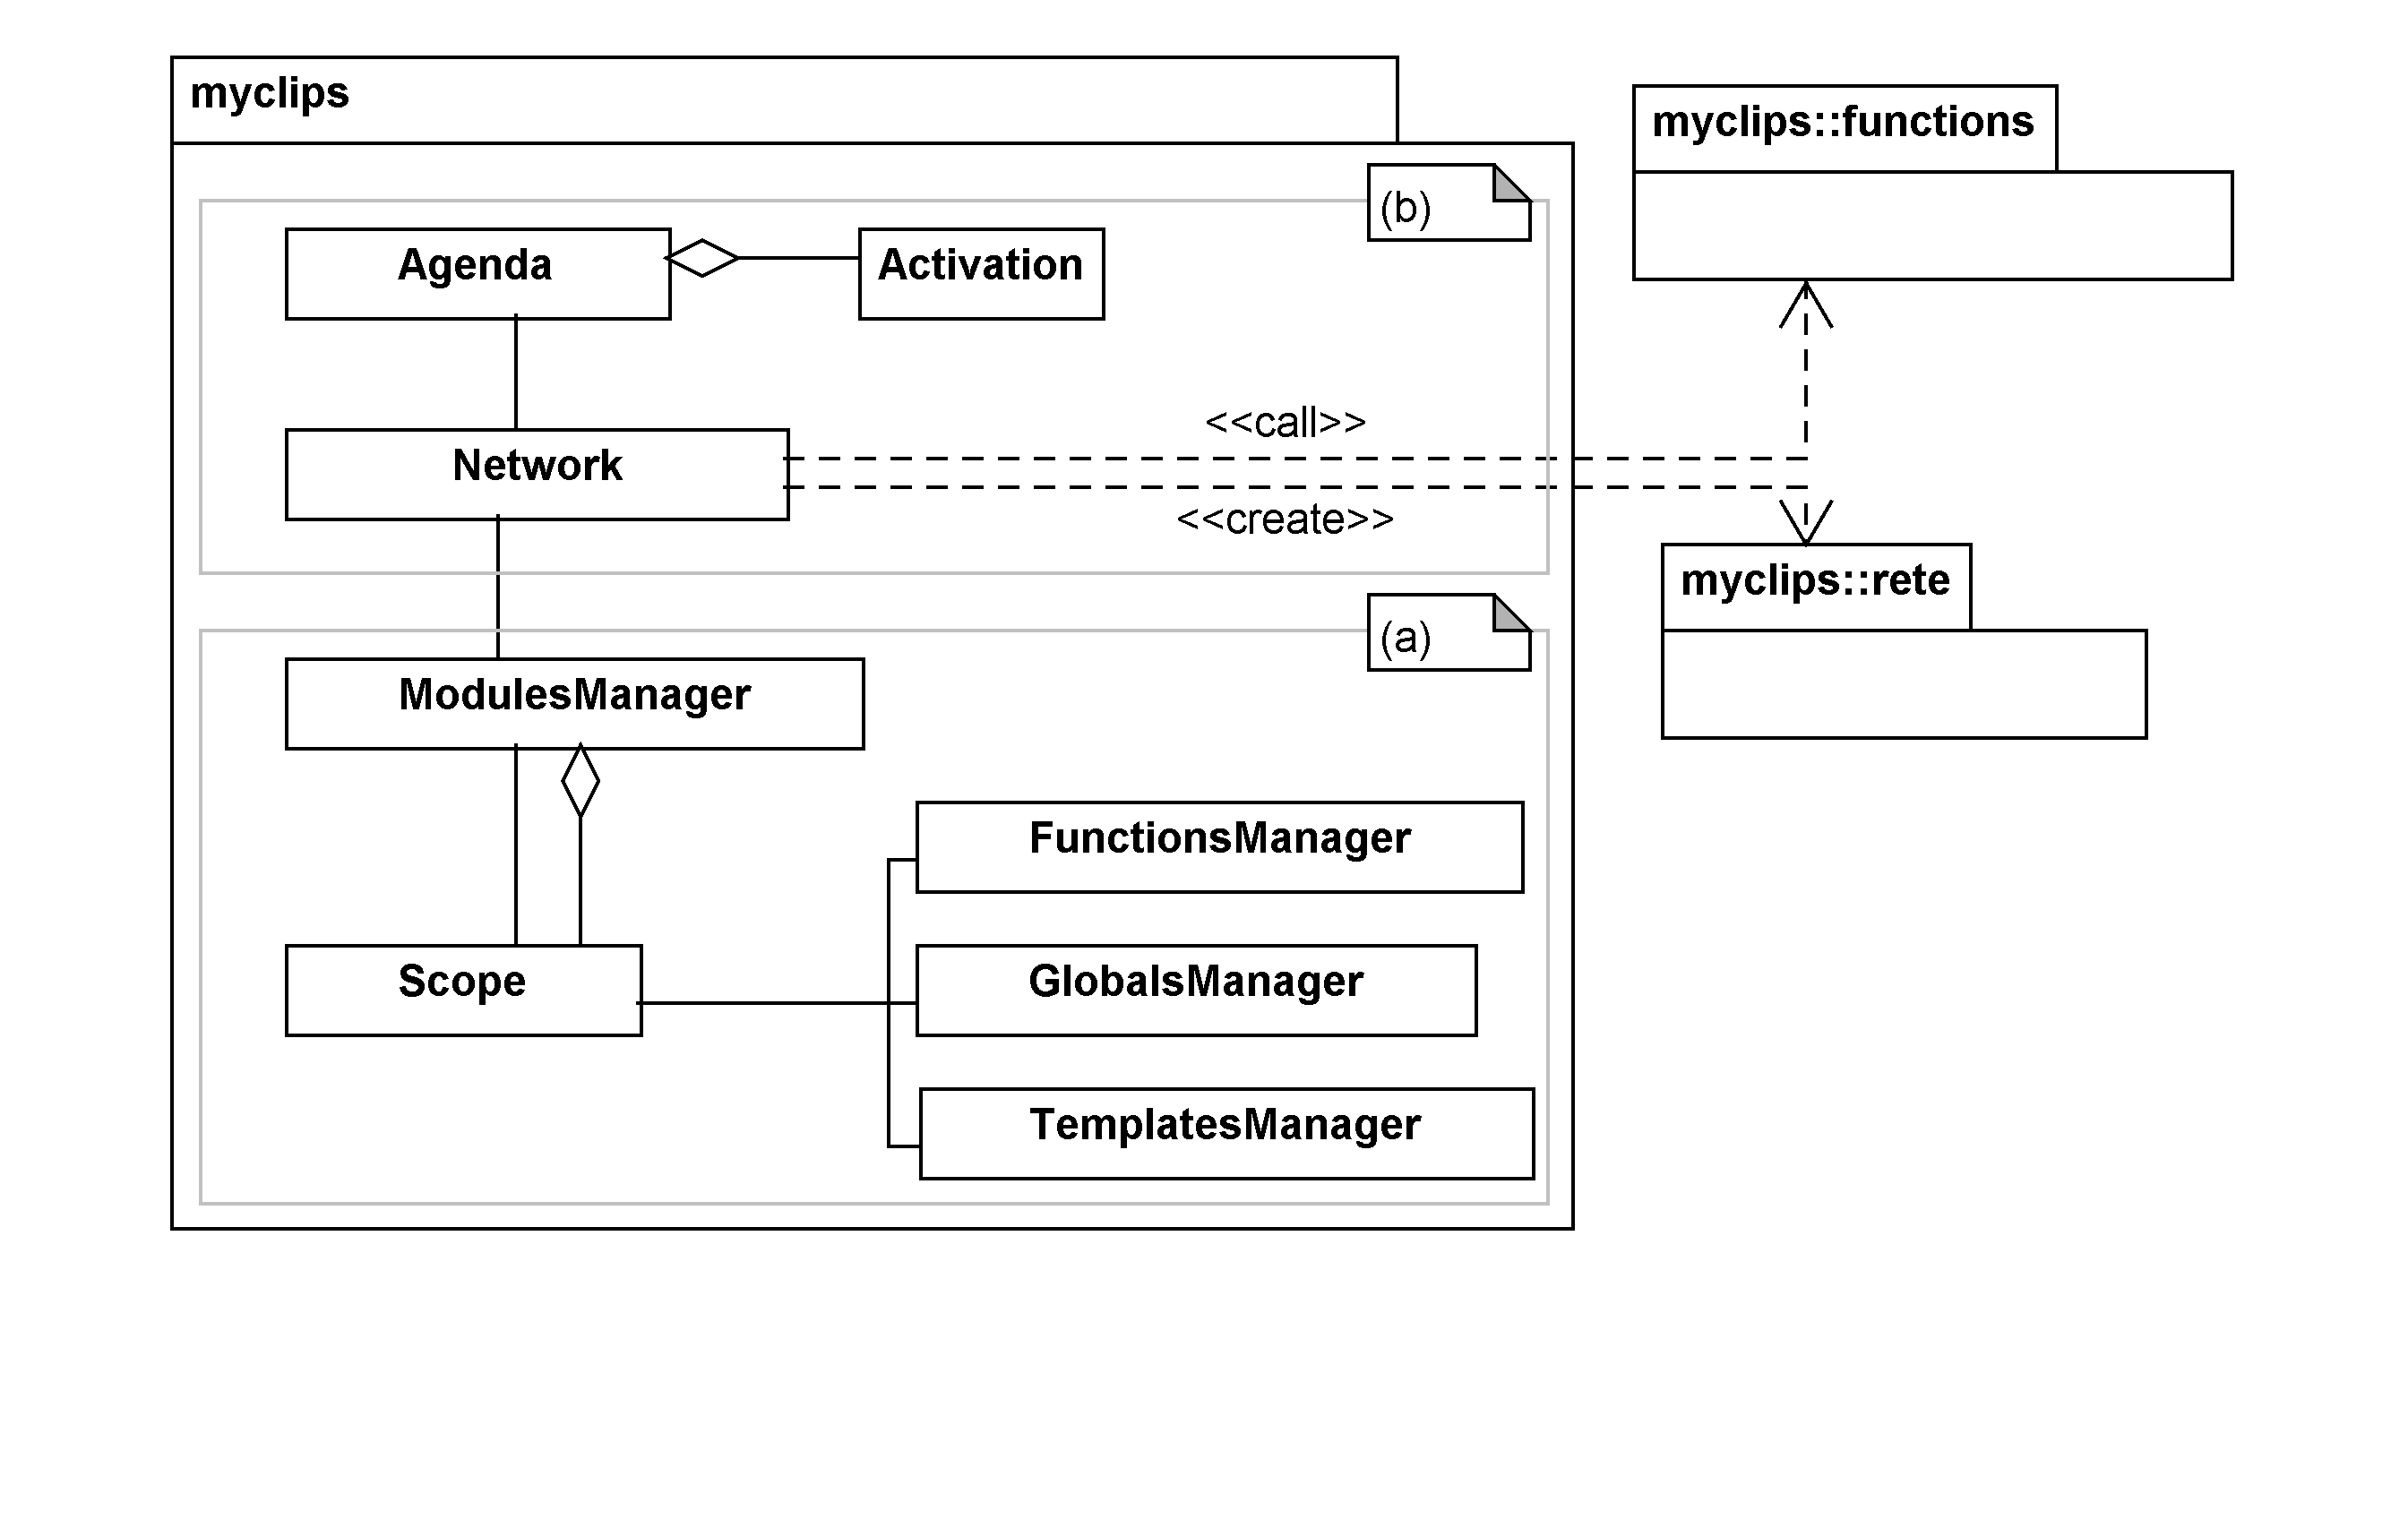
\includegraphics[width=1\textwidth]{Immagini/Capitolo3/Packages/IE.png}
\caption{Package \emph{myclips}: vista degli elementi che collaborano per la realizzazione dei servizi dell'\emph{IE}}\label{fig:packages-ie}
\end{figure}

Il ruolo del modulo \emph{Motore Inferenziale} (IE) è quello di offrire i servizi principali relativi alla gestione delle definizioni, all'esecuzione del ciclo \emph{recognize-act} e alla gestione delle transizioni fra gli stati del sistema.

L'insieme dei servizi viene realizzato attraverso una collaborazione fra classi. A livello logico, le classi possono essere raggruppate in due sezioni: una prima adibita alla gestione delle definizioni del sistema esperto (\emph{(a)} in \figurename~\ref{fig:packages-ie}), una seconda alla interpretazione e esecuzione dei costrutti (\emph{(b)} in \figurename~\ref{fig:packages-ie}).

\begin{figure}[h]
\centering
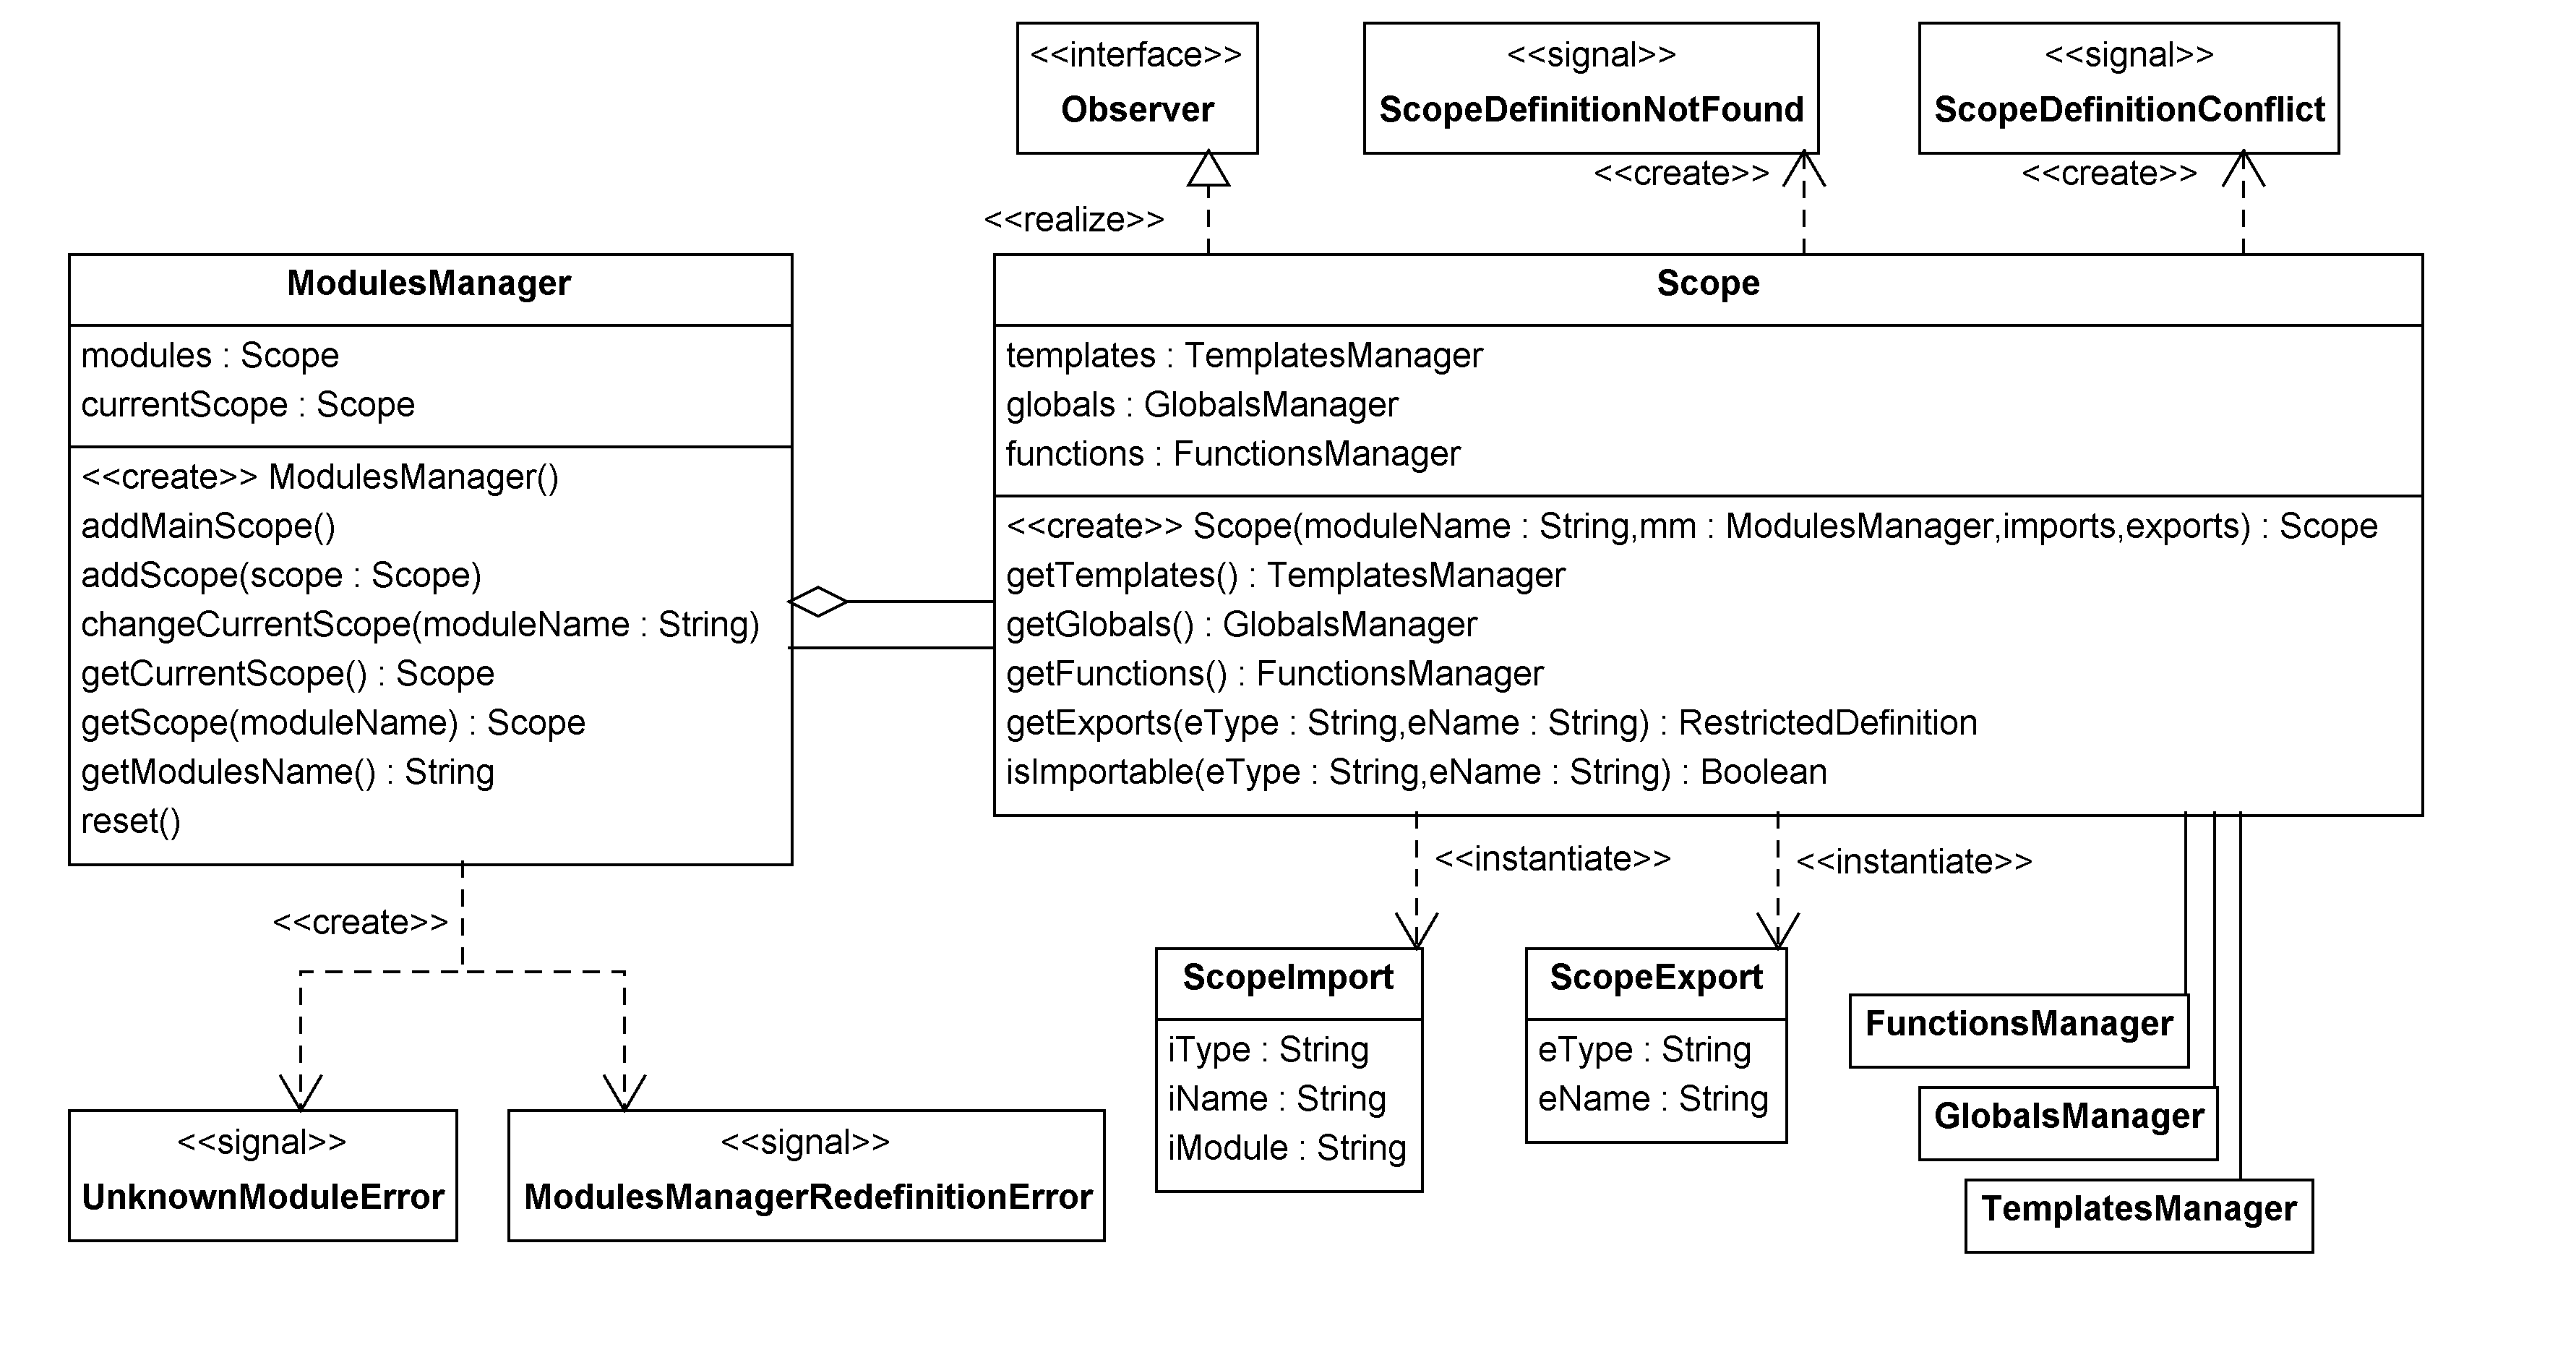
\includegraphics[width=1\textwidth]{Immagini/Capitolo3/Classi/myclips_Scope-ModulesManager.png}
\caption{Package \emph{myclips}: vista delle classi per la gestione dei moduli}\label{fig:class-myclips-scope-mm}
\end{figure}

\paragraph{Gestione delle definizioni}

La gestione dei moduli è affidata alla collaborazione fra le classi \emph{Scope} e \emph{ModulesManager}~(\figurename~\ref{fig:class-myclips-scope-mm}).
La classe \emph{ModulesManager} memorizza l'insieme dei moduli definiti in un sistema esperto e un attributo di stato (\emph{currentScope}) nel quale viene memorizzato il riferimento allo \emph{Scope} rappresentante il contesto corrente di esecuzione del sistema. Le definizioni o le azioni alle quali non è stato attribuito esplicitamente un modulo di appartenenza vengono automaticamente relazionate con il modulo corrente.

Le istanze di classe \emph{Scope} rappresentano singoli moduli definiti nel sistema. A differenza dell'entità \emph{modulo} intesa come collezione di costrutti e definizioni definiti nel \emph{modulo} stesso, quella di \emph{Scope} raggruppa l'insieme di definizioni disponibili in un preciso contesto d'uso relazionato ad un modulo. Ogni \emph{Scope} possiede i riferimenti ai manager dei tipi di costrutti definibili e gestisce il protocollo di \emph{import/export} delle definizioni~(\figurename~\ref{fig:sequence-def-import-export}).

\begin{figure}
\centering
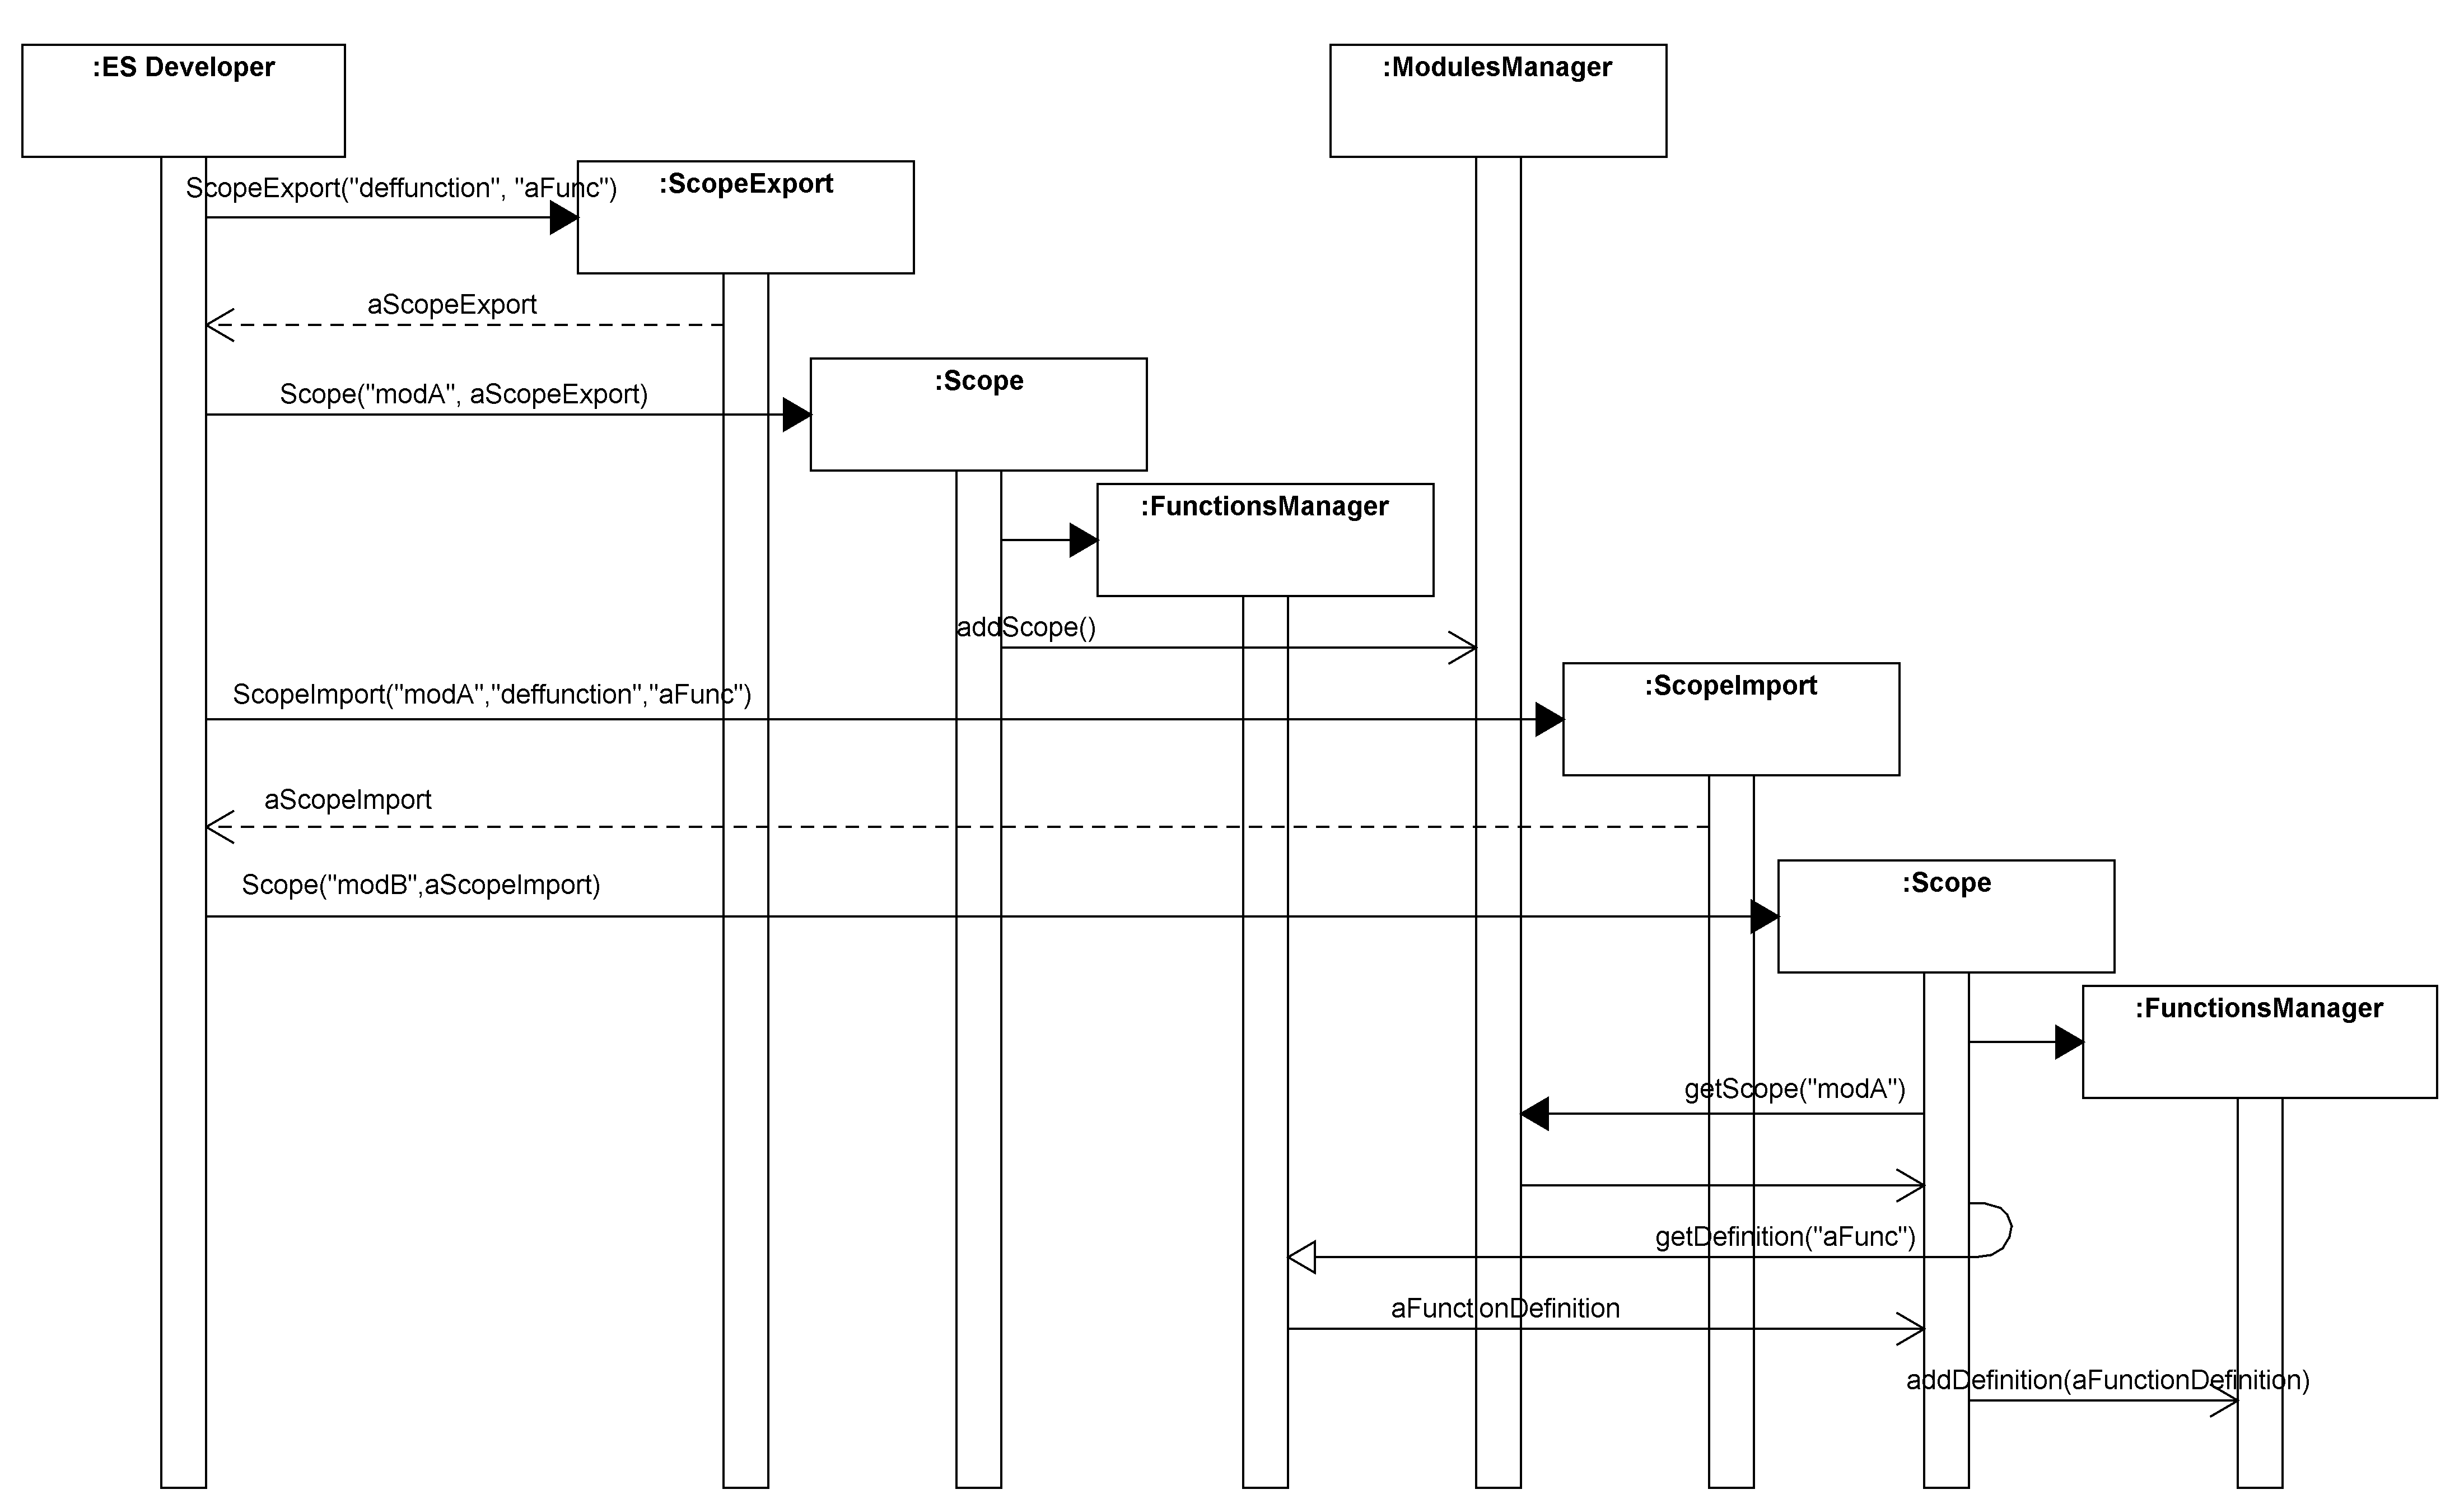
\includegraphics[width=1.2\textwidth, angle=270]{Immagini/Capitolo3/Sequenza/myclips_Scope_ImportExport.png}
\caption[Diagramma di sequenza \emph{import/export} delle definizioni]{Diagramma di sequenza \emph{import/export} delle definizioni: le clausule di importazione o esportazione determinano lo scambio di definizioni fra moduli}\label{fig:sequence-def-import-export}
\end{figure}

\begin{figure}
\centering
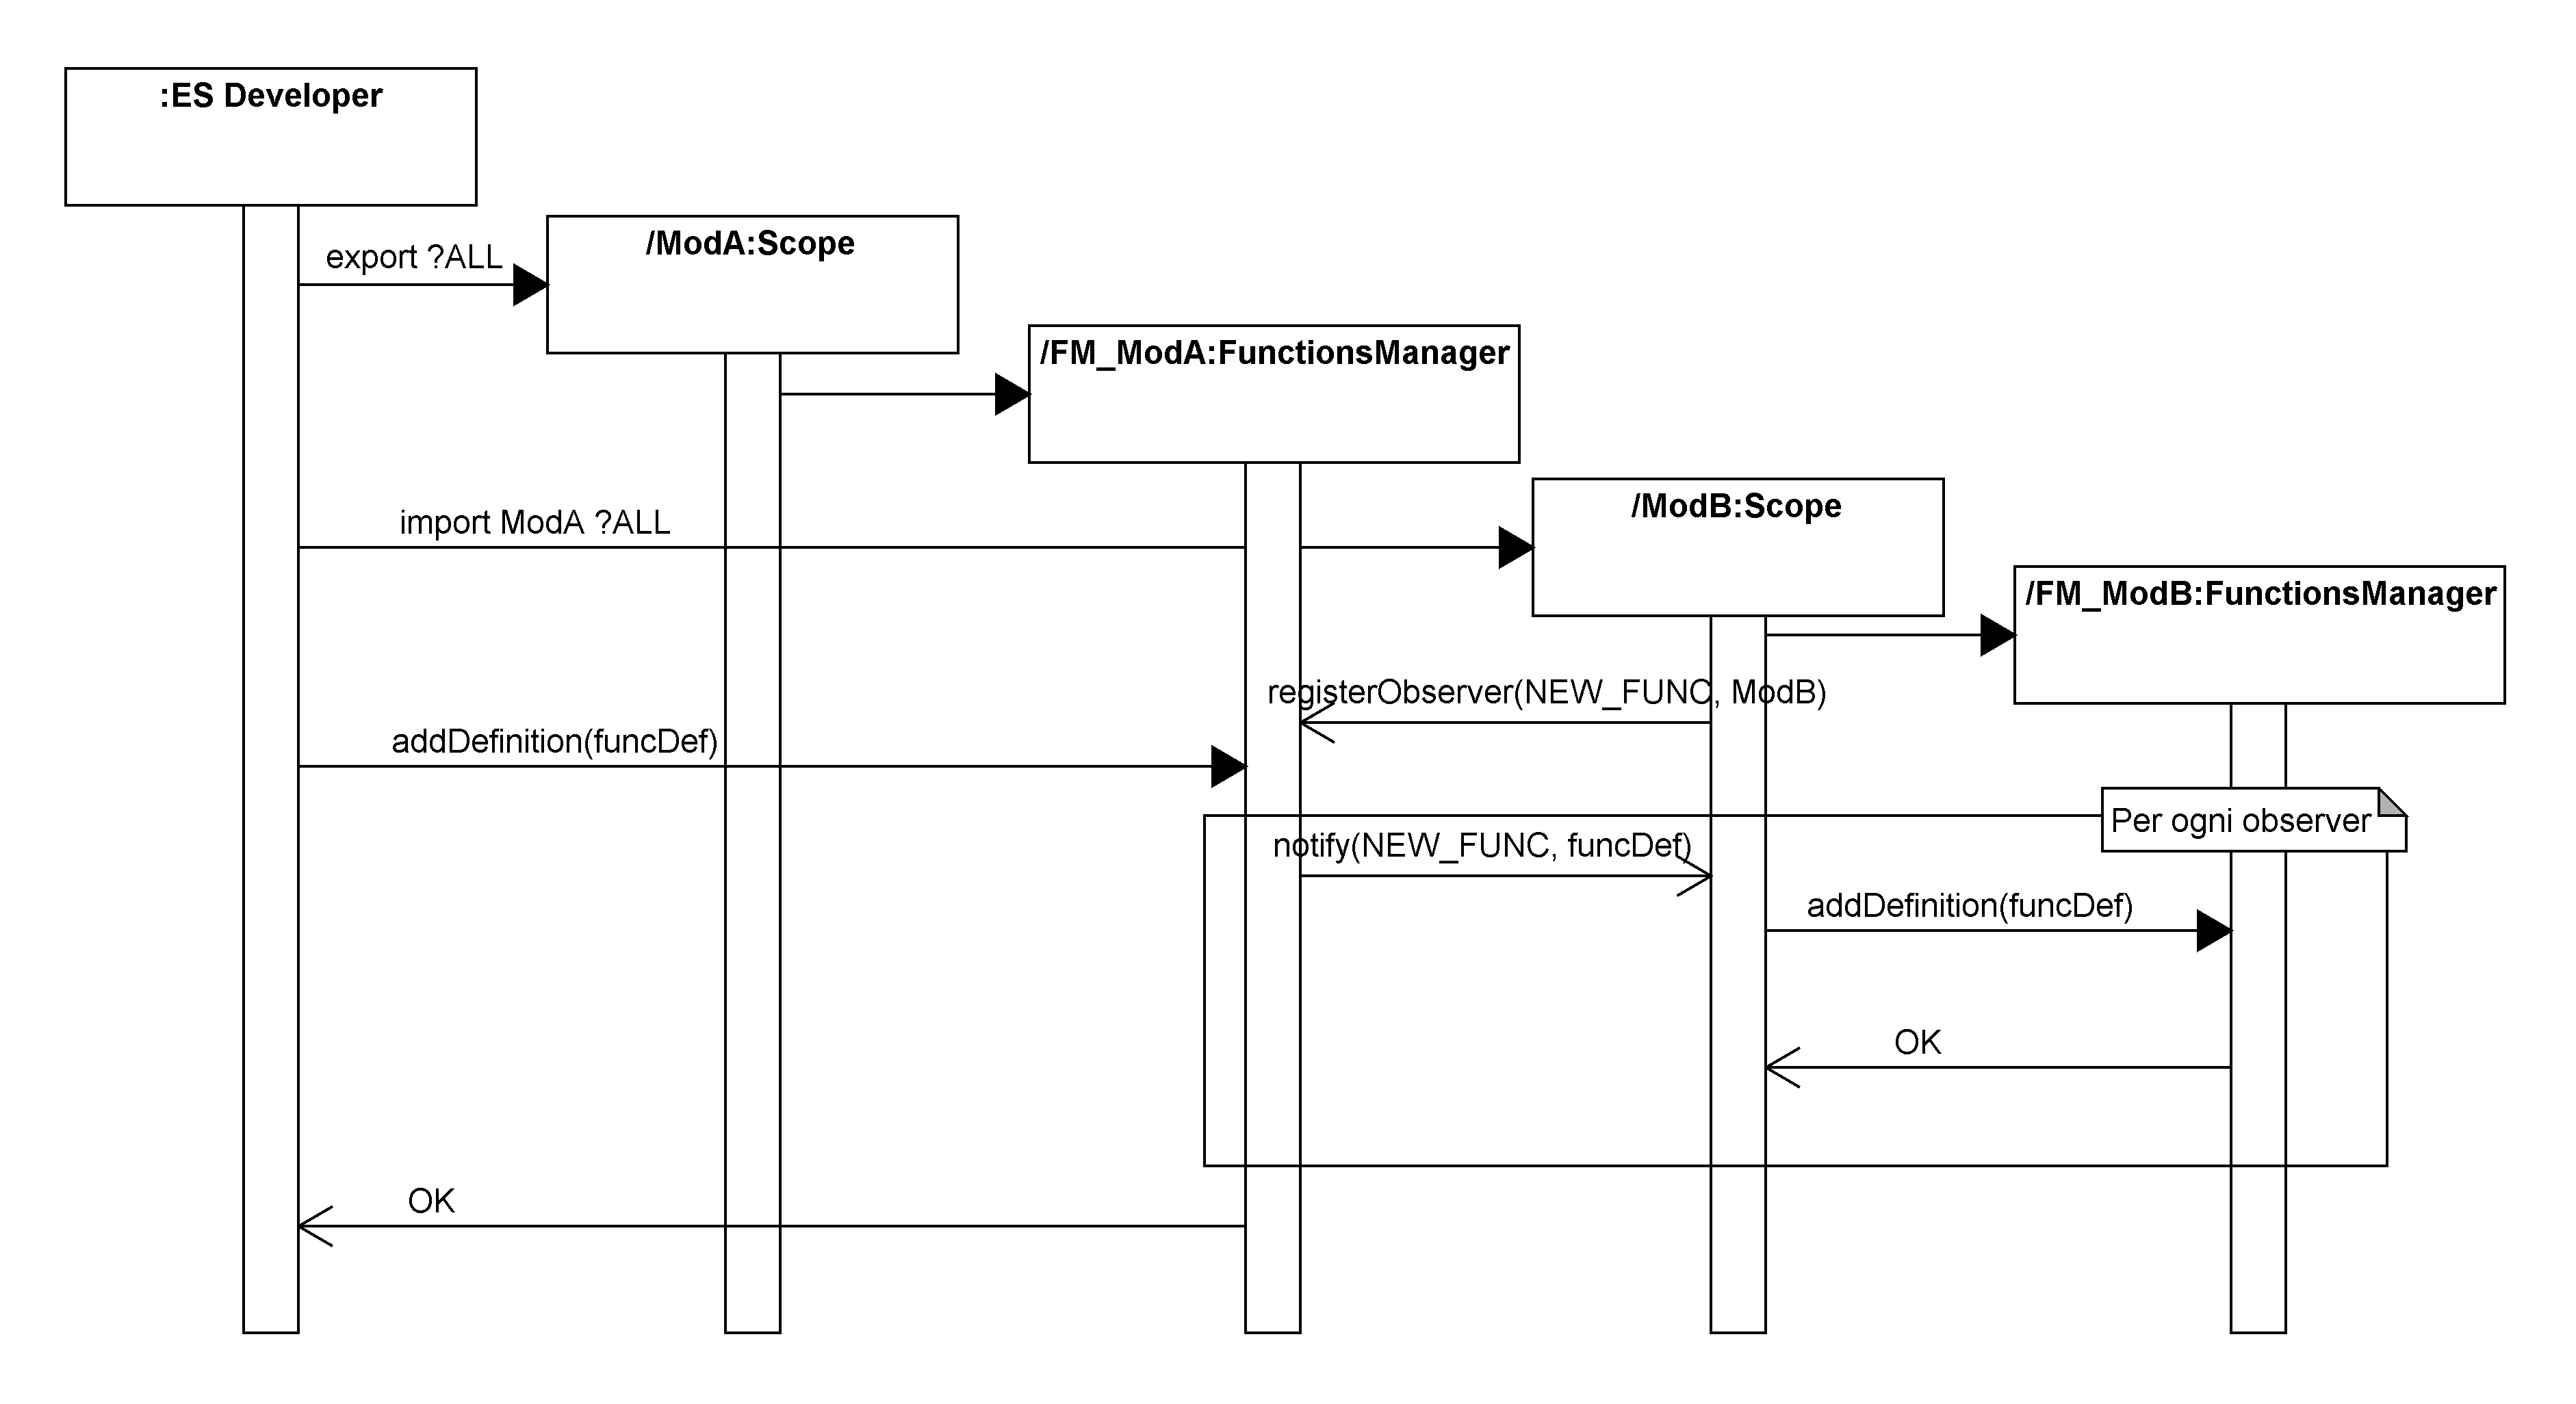
\includegraphics[width=1.3\textwidth, angle=270]{Immagini/Capitolo3/Sequenza/myclips_Scope_ExportPromise.png}
\caption[Diagramma di sequenza \emph{import/export} tramite l'uso di \emph{promesse}]{Diagramma di sequenza \emph{import/export} tramite l'uso di \emph{promesse}: i moduli vengono relazionati e l'aggiunta successiva di definizioni al primo modulo viene automaticamente inoltrata al secondo modulo}\label{fig:sequence-def-import-export-promise}
\end{figure}

Lo scambio di definizioni non ancora esplicitate avviene attraverso l'utilizzo delle \emph{promesse di import/export}. Nel momento in cui un modulo \emph{modA} definisce tutti i propri costrutti esportabili ed un secondo modulo \emph{modB} esplicita la volontà di importare tutti i costrutti di \emph{modA} si fa uso di una \emph{promessa}: il protocollo prevede l'utilizzo di una soluzione basata sul pattern \emph{observer-observable} per eseguire il trasferimento delle definizioni aggiunte in fasi successive~(\figurename~\ref{fig:sequence-def-import-export-promise}).
\pagebreak

\begin{figure}
\centering
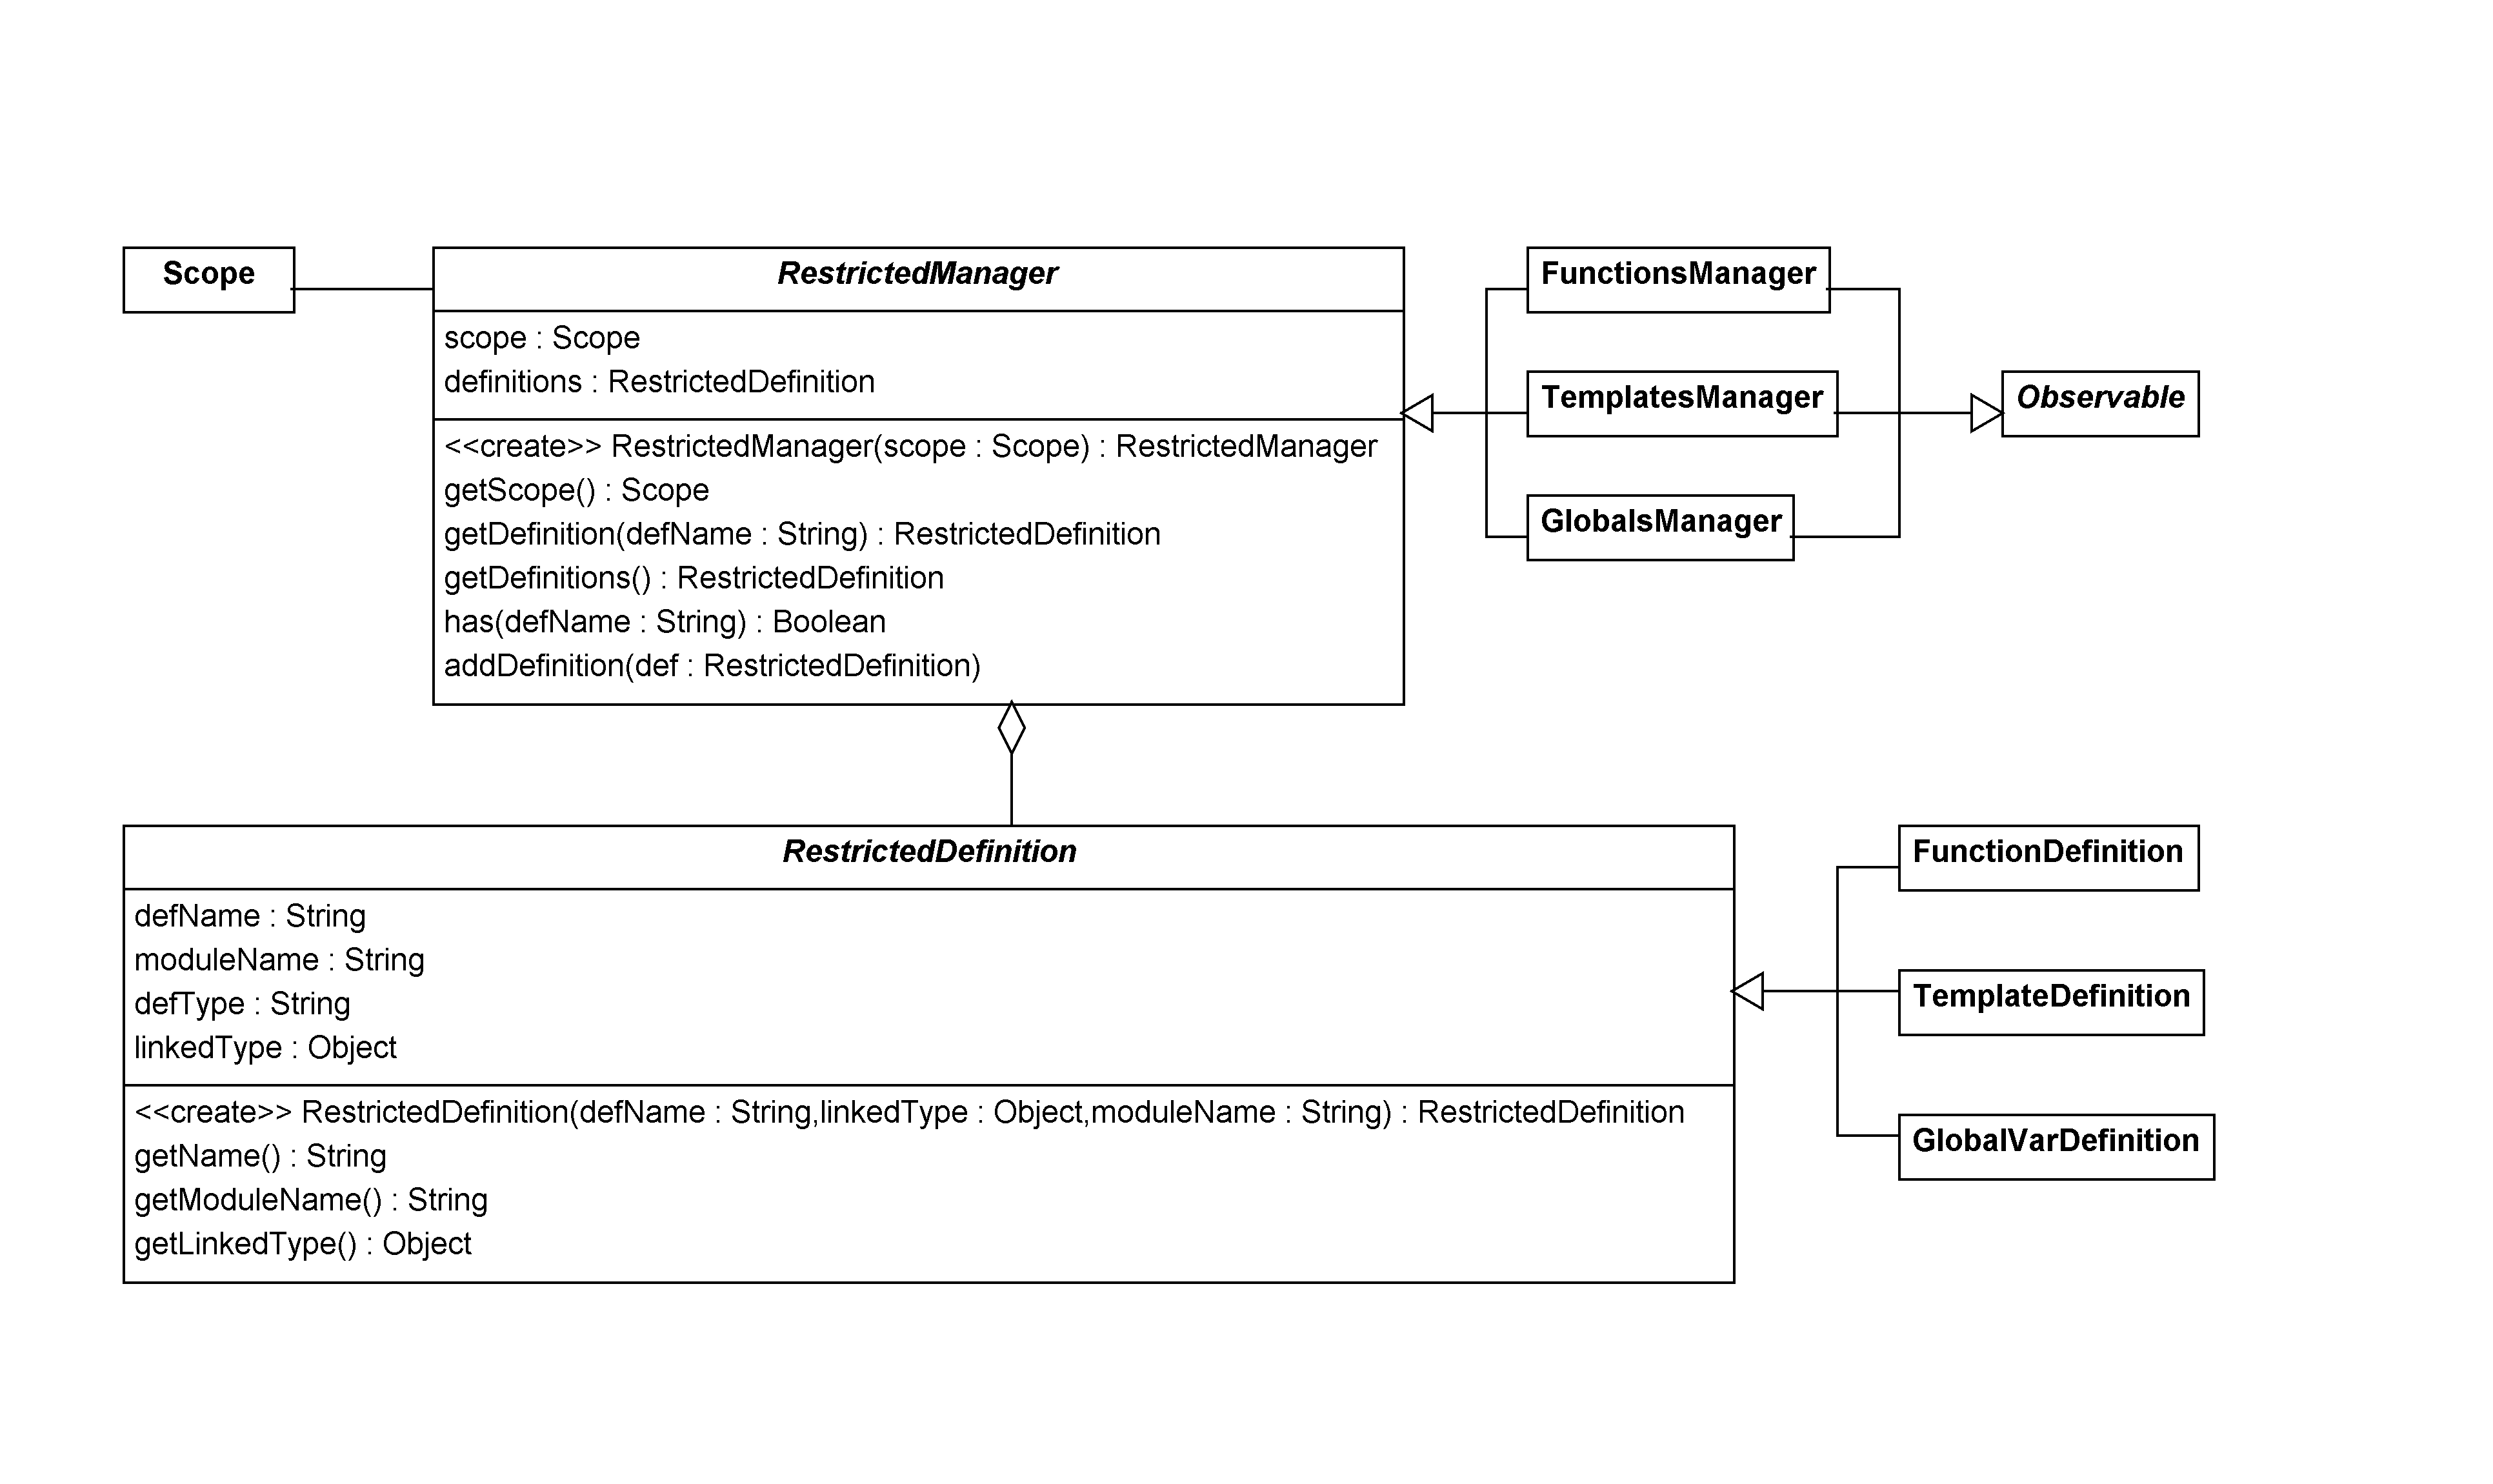
\includegraphics[width=1.2\textwidth]{Immagini/Capitolo3/Classi/myclips_RestrictedManager.png}
\caption{Vista delle classi \emph{manager} di definizioni}\label{fig:class-myclips-restricted-manager}
\end{figure}

La memorizzazione delle definizioni è affidata alle classi \emph{GlobalsManager}, \emph{TemplatesManager} e \emph{FunctionsManager}~(\figurename~\ref{fig:class-myclips-restricted-manager}). 
Ogni \emph{manager} memorizza un preciso tipo di definizioni che possono essere utilizzate nell'ambito di uno \emph{Scope} specifico. L'eventuale presenza di \emph{promesse di export} viene valutata durante l'aggiunta di nuove definizioni nei \emph{manager}~(\figurename~\ref{fig:sequence-def-import-export-promise}).


\paragraph{Gestione dell'inferenza}

\begin{figure}
\centering
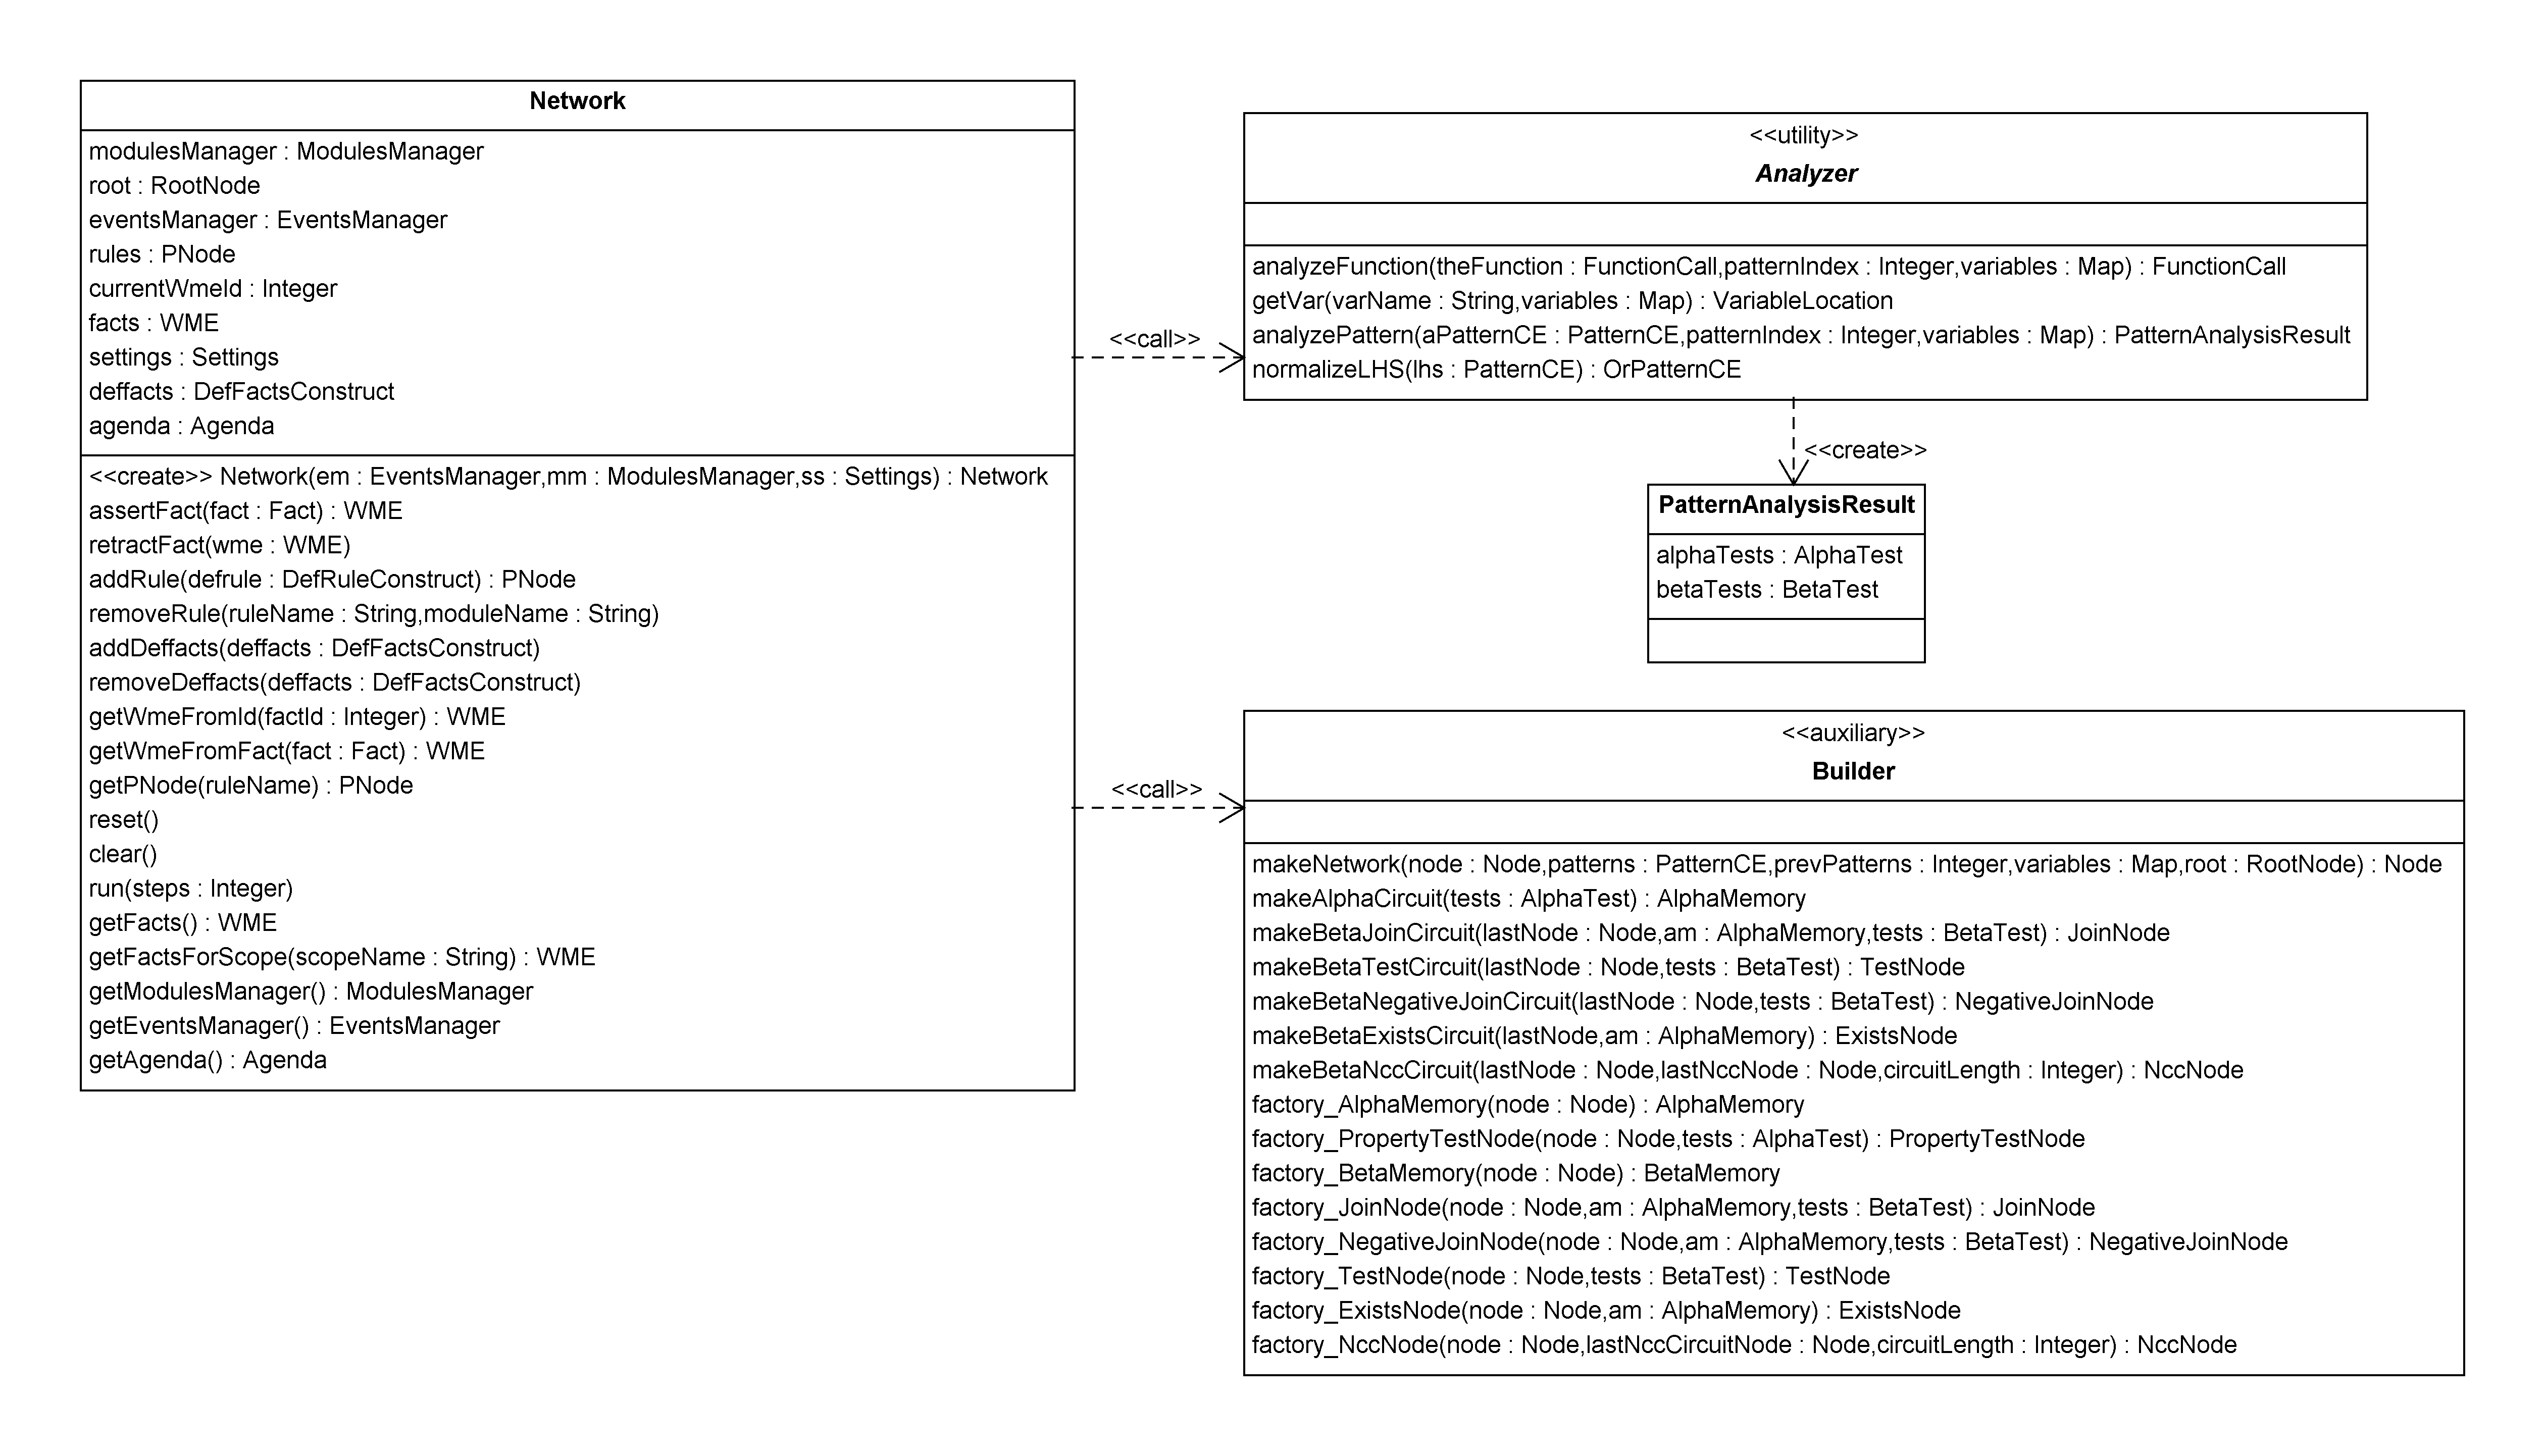
\includegraphics[width=1\textwidth]{Immagini/Capitolo3/Classi/myclips_rete_Network.png}
\caption{Package \emph{myclips}: vista della classe \emph{Network}}\label{fig:class-myclips-network}
\end{figure}

La classe principale per la gestione dell'inferenza è la classe \emph{fa\c{c}ade} \emph{Network}~(\figurename~\ref{fig:class-myclips-network}): astraendo dalla complessità delle interfacce offerte dal \emph{matcher}, offre metodi per la manipolazione del \emph{rules-set}, dei fatti iniziali e della \emph{working-memory}. Realizzando il ciclo \emph{recognize-act} al suo interno, permette l'utilizzo dei meccanismi di inferenza offerti dal sistema. La classe si affida a due componenti \emph{utility} per la reale implementazione delle funzionalità di compilazione e analisi delle regole interfacciandosi con il modulo \emph{matcher}, descritto in seguito.


\begin{figure}
\centering
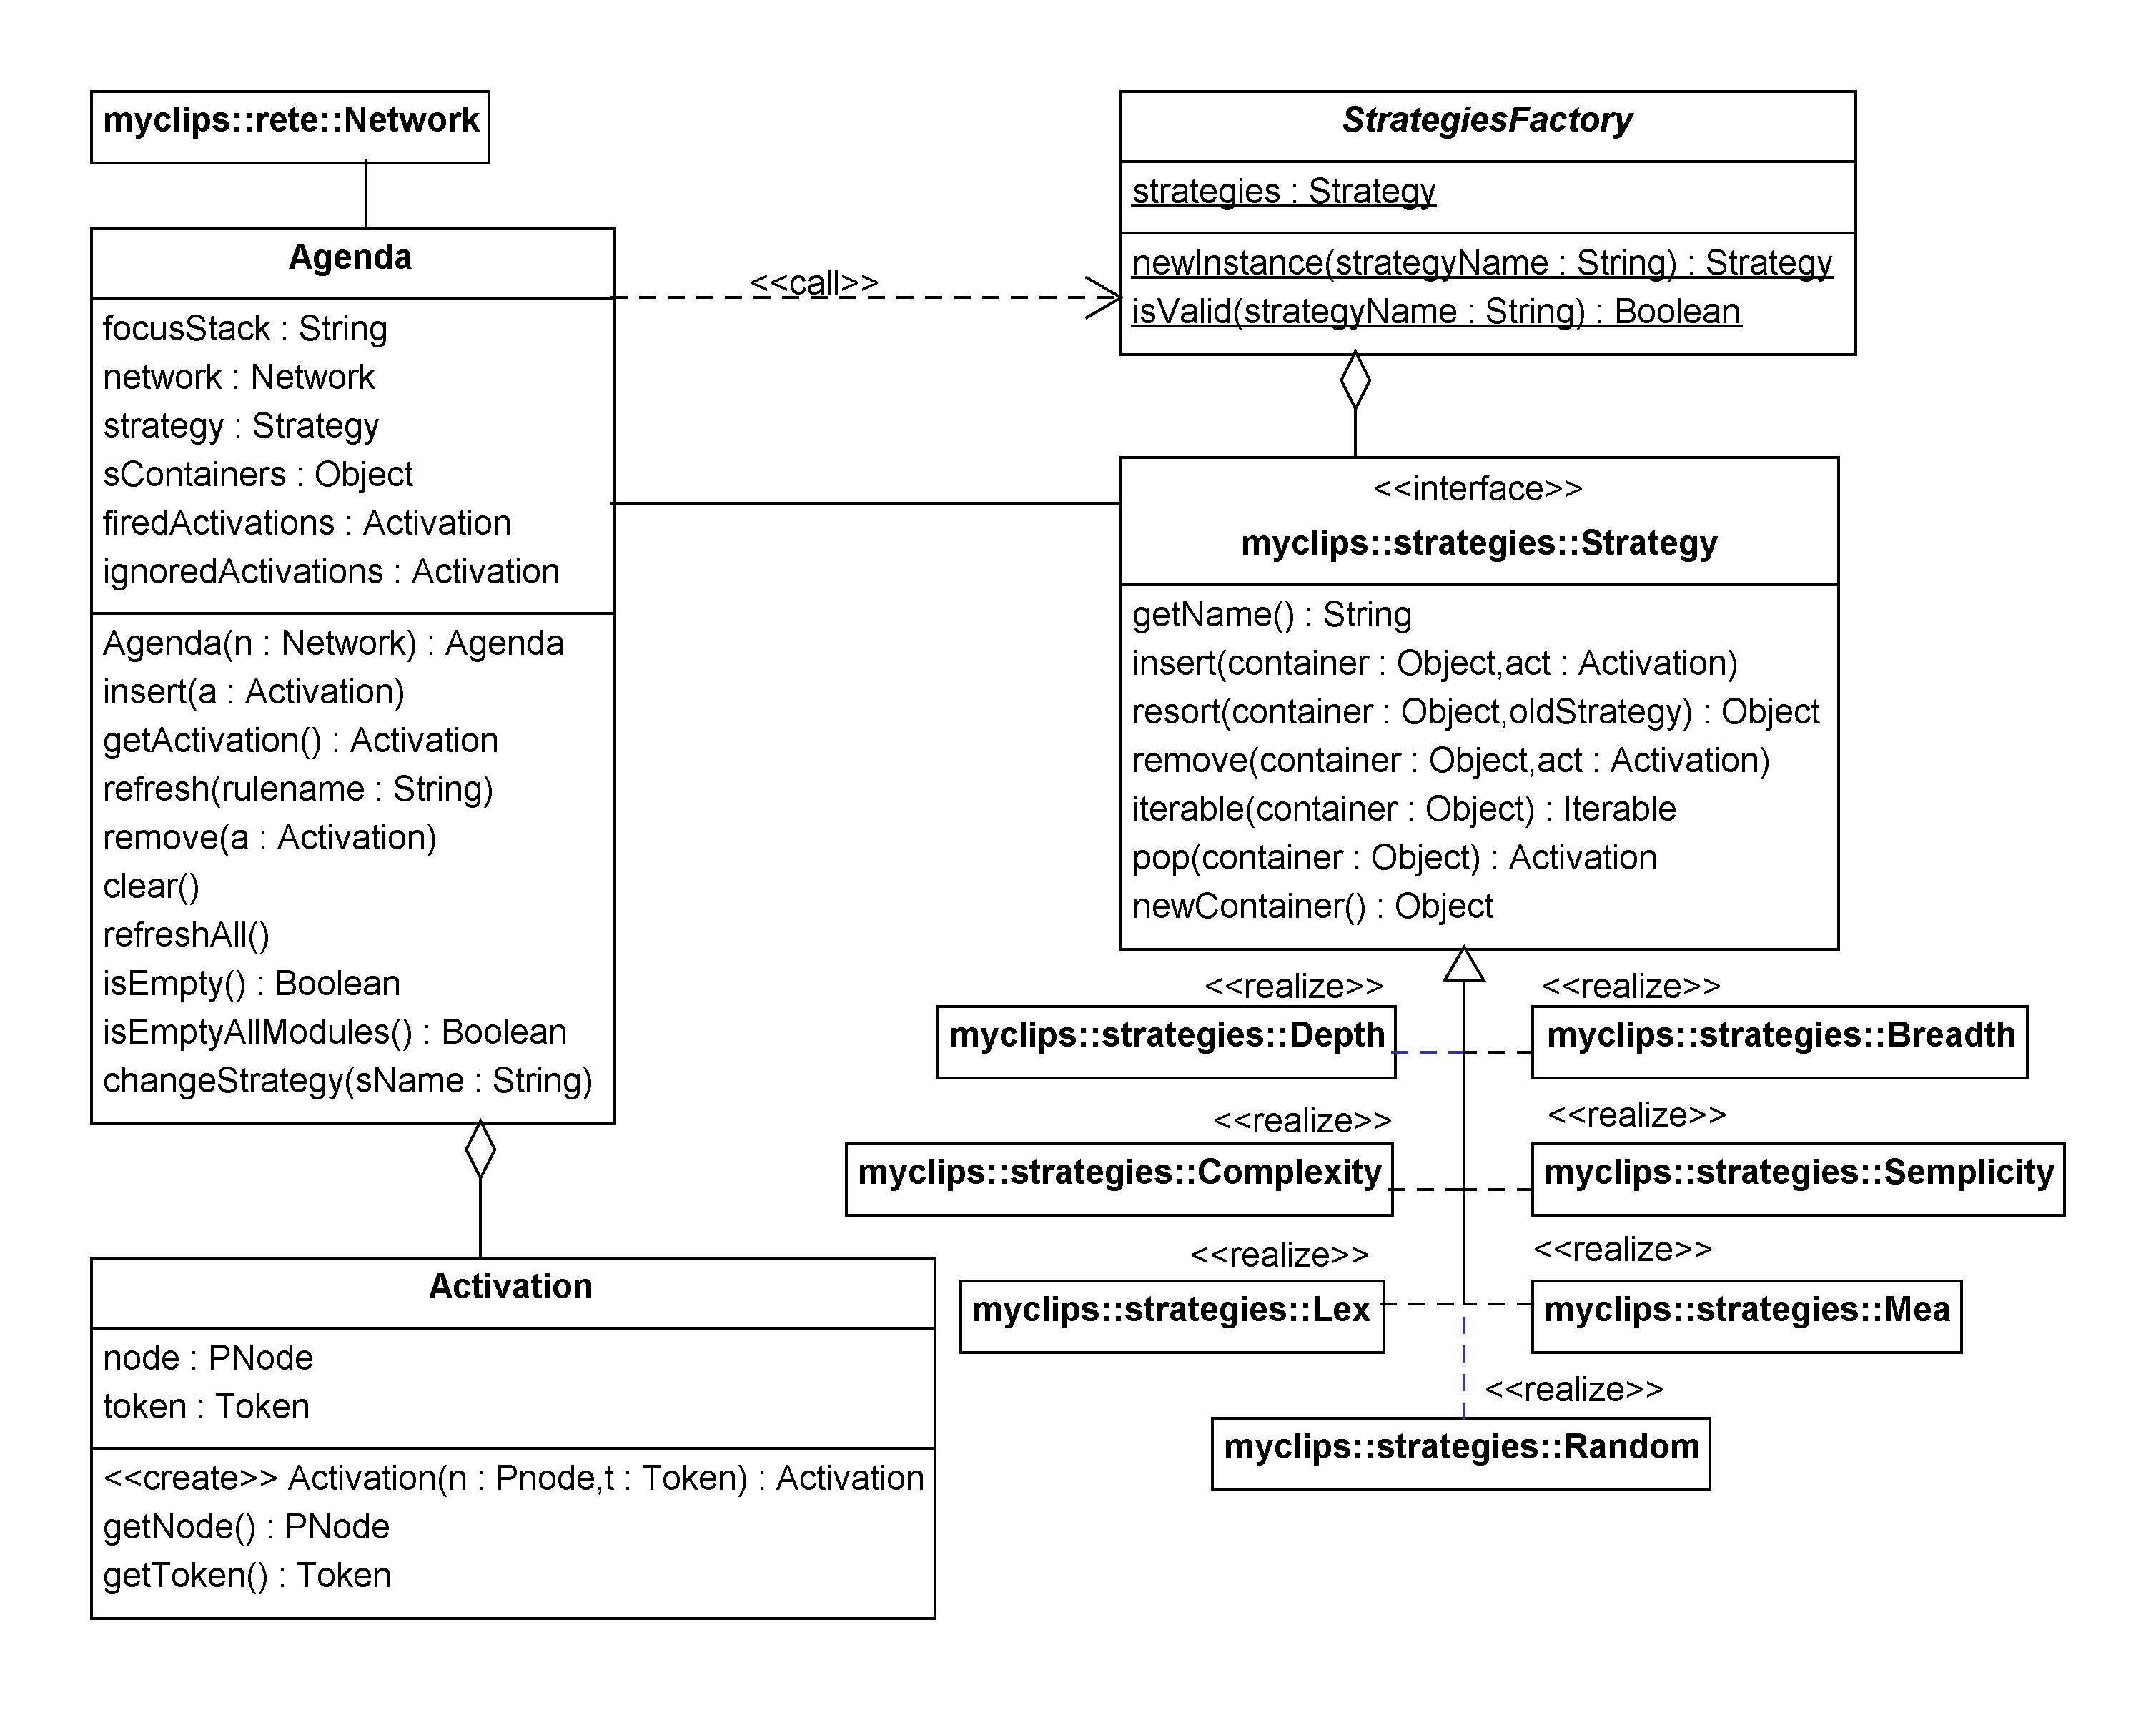
\includegraphics[width=1\textwidth]{Immagini/Capitolo3/Classi/myclips_Agenda-Strategies.png}
\caption{Package \emph{myclips}: vista delle classi e interfacce relative ad  \emph{Agenda} e \emph{Strategie} (CRS)}\label{fig:class-myclips-agenda-strategies}
\end{figure}

La gestione delle attivazioni viene affidata alla classe \emph{Agenda} e al \emph{package} \emph{myclips.strategies}~(\figurename~\ref{fig:class-myclips-agenda-strategies}). La classe organizza le attivazioni, offrendo servizi per l'aggiunta o la rimozione delle stesse, e gestendo le strategie di risoluzione dei conflitti. La collaborazione fra \emph{Agenda} e \emph{Strategy} viene realizzata attraverso l'utilizzo del pattern \emph{Factory}: la creazione dell'istanza di strategia viene delegata ad una istanza \emph{Singleton} della classe \emph{StrategiesFactory}, la quale inizializza un'implementazione dell'interfaccia \emph{Strategy} fornita basandosi su un id di strategia. L'implementazione dell'\emph{Agenda} viene realizzata tenendo conto dei metodi forniti dall'interfaccia, astraendo dall'implementazione concreta. Le strutture dati adibite alla memorizzazione delle sequenze di attivazioni vengono inizializzate e concretamente gestite dalla specifica implementazione della \emph{Strategy}.


\subsubsection{Modulo Matcher}
Lo scopo del modulo \emph{matcher} è quello di confrontare lo stato della \emph{working-memory} con il \emph{rule-set} identificando l'insieme di attivazioni disponibili e inserendole nell'\emph{agenda delle attivazioni}.

\begin{figure}
\centering
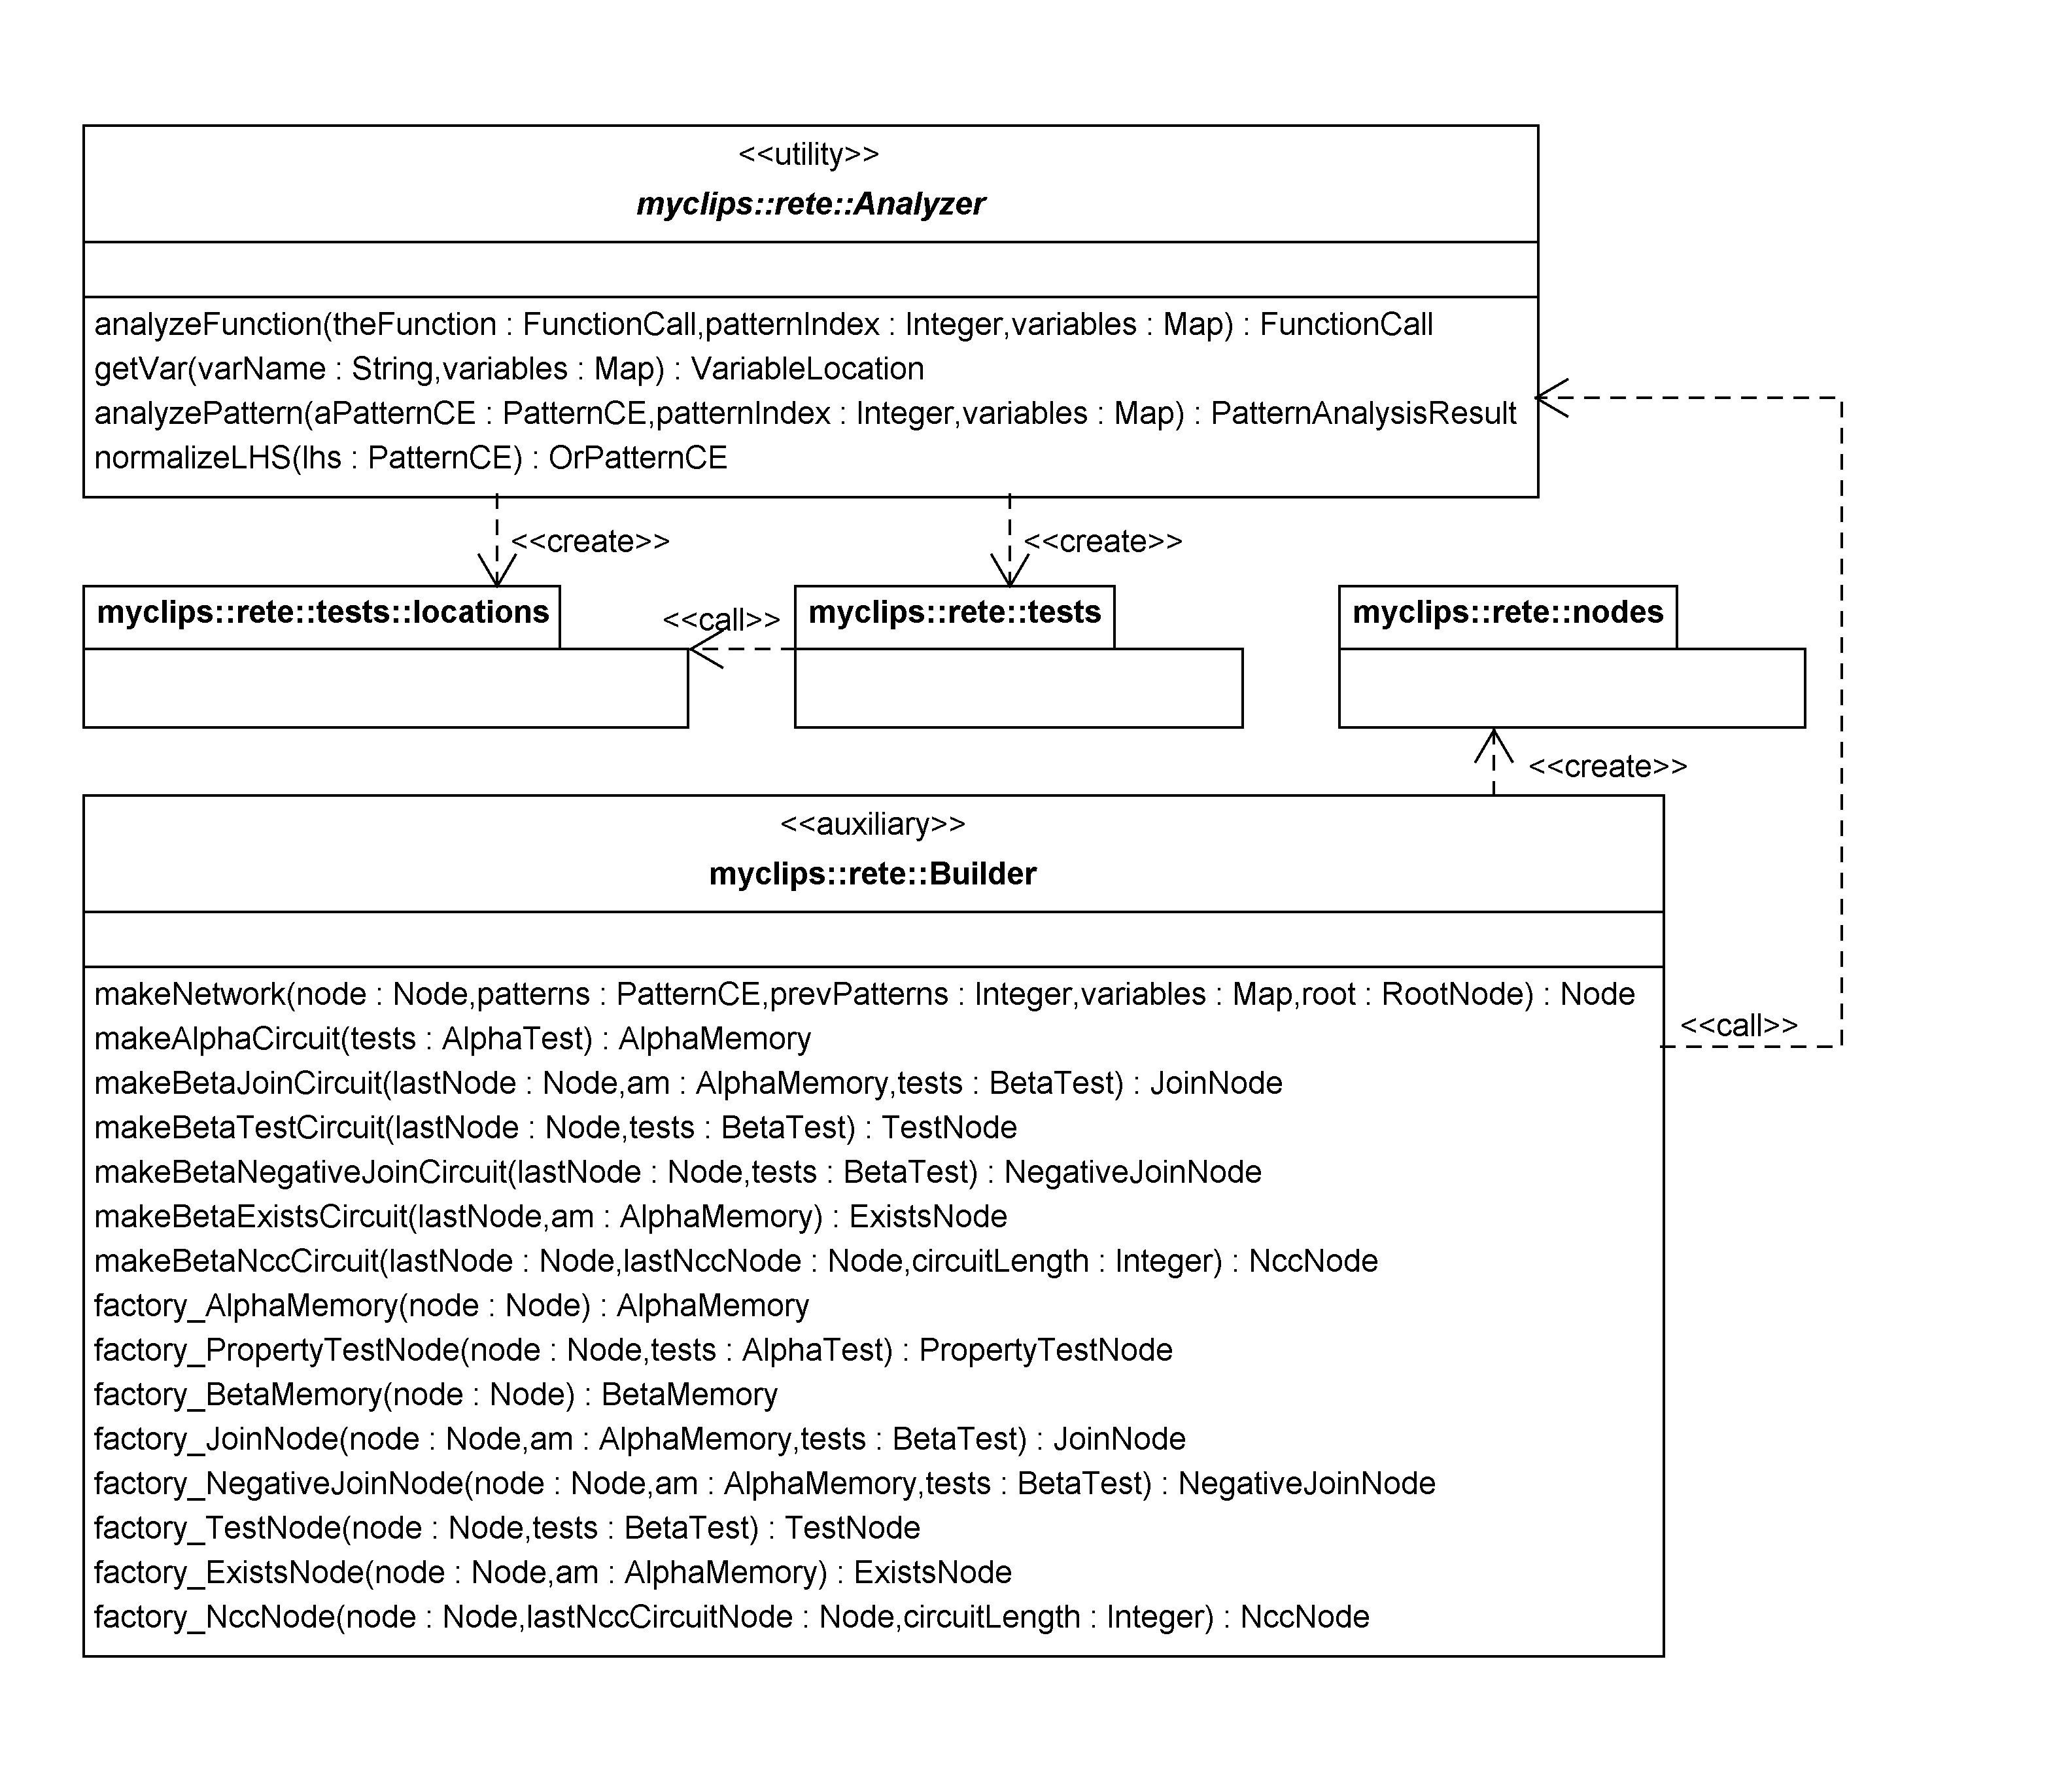
\includegraphics[width=1.2\textwidth]{Immagini/Capitolo3/Classi/myclips_rete_Builders.png}
\caption{Package \emph{myclips.rete}: vista delle classi utility per la conversione delle regole in strutture di RETE}\label{fig:class-myclips-rete-builders}
\end{figure}

Il modulo si basa sull'utilizzo di un'implementazione interpretata dell'algoritmo RETE. Attraverso l'uso di due classi utility~(\figurename~\ref{fig:class-myclips-rete-builders}) per analisi dei \emph{pattern} delle regole e per la costruzione del grafo, il \emph{rules-set} viene convertito nel grafo esplicito di valutazione caratteristico dell'algoritmo RETE.

La classe \emph{Analyzer} viene utilizzata per manipolare la forma dei pattern delle regole nel \emph{rules-set}, adattandole alla topologia del grafo di RETE, e individuare l'insieme dei test \emph{alpha} e \emph{beta} per i pattern, inizializzando le relative istanze delle classi di test organizzate nel package \emph{myclips.rete.tests}.

La classe \emph{Builder} ha invece il compito di creare l'insieme di nodi necessari alla costituzione del grafo, associandoli dove necessario ai test ottenuti dall'\emph{Analyzer}.
L'utilizzo dei metodi \emph{factory} per i nodi, come alternativa a normali costruttori, permette di utilizzare istanze condivise dei nodi quando possibile.

\paragraph{Nodi del grafo di RETE}

Il set di nodi che supportano l'implementazione dell'algoritmo RETE sono realizzazioni di un set di interfacce fondamentali (\figurename~\ref{fig:class-myclips-rete-interfaces}) che hanno il compito di formalizzare i metodi usati dai nodi per lo scambio di segnali e rendere possibile l'attraversamento da parte dei \emph{Token}.

\begin{figure}
\centering
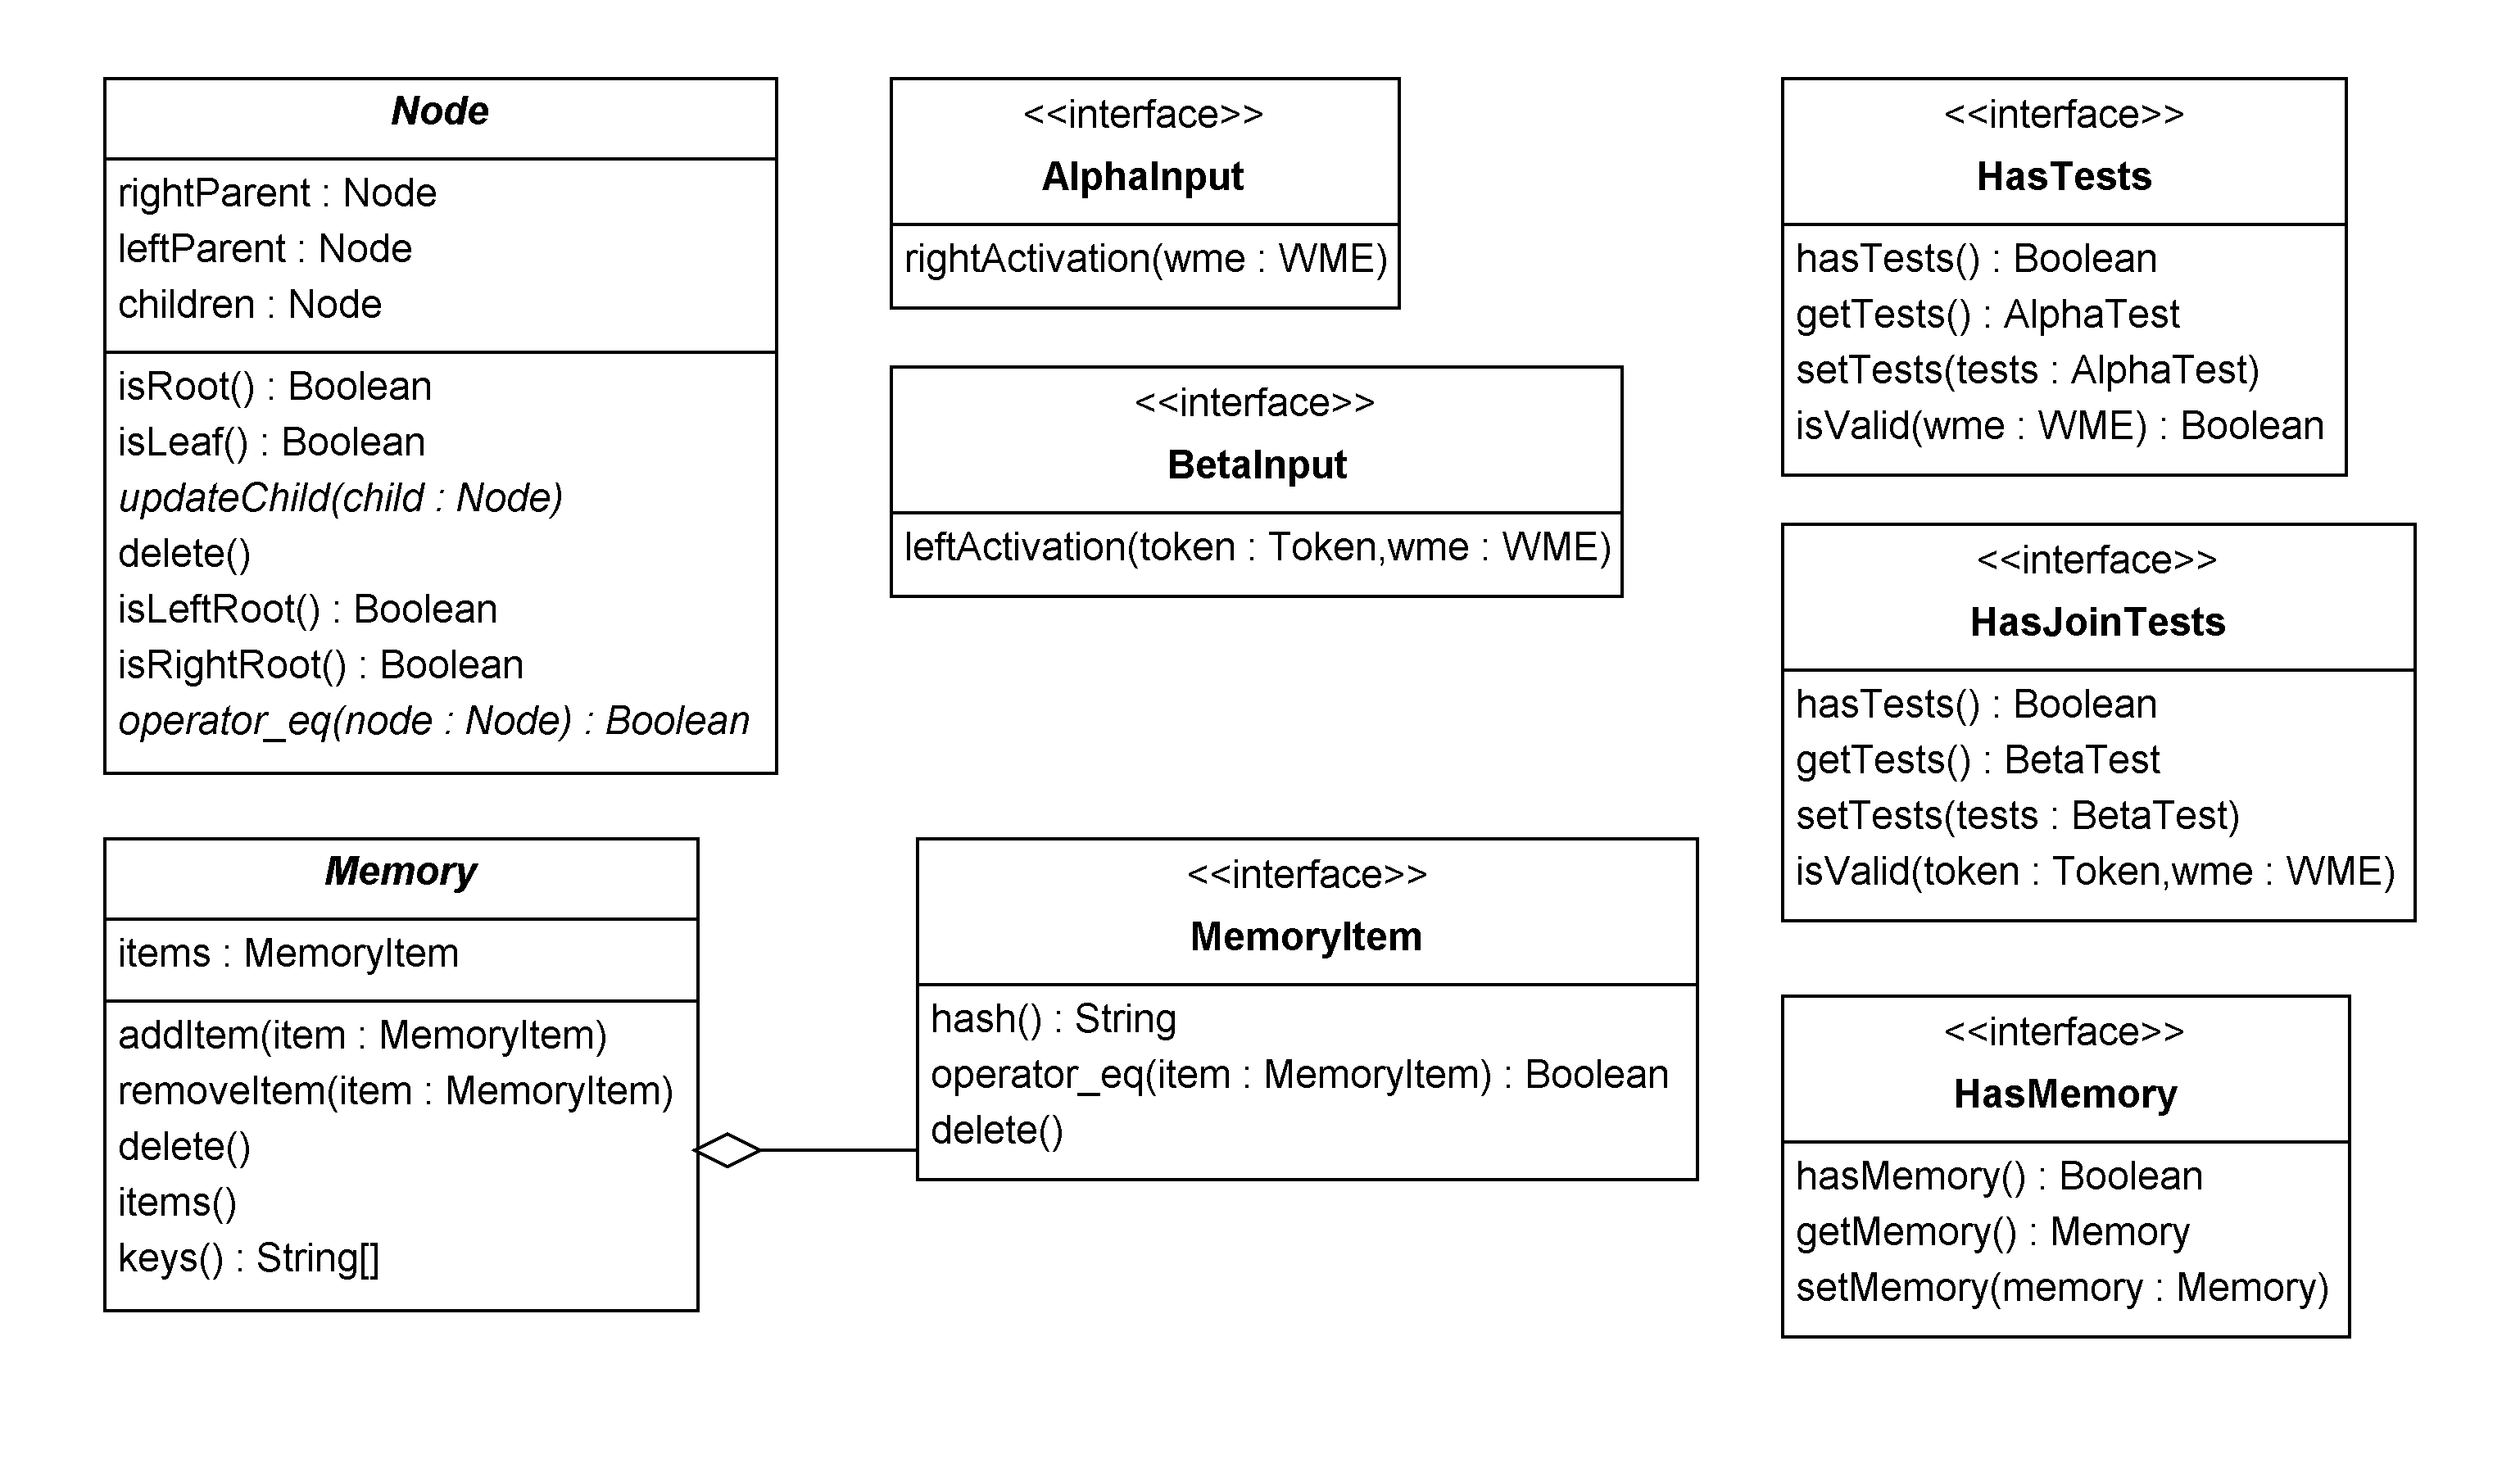
\includegraphics[width=1\textwidth]{Immagini/Capitolo3/Classi/myclips_rete_Interfacce.png}
\caption{Package \emph{myclips.rete}: vista delle interfacce di base usate dai nodi per l'implementazione di RETE}\label{fig:class-myclips-rete-interfaces}
\end{figure}

La classe astratta \emph{Node}, specializzata da tutti i nodi, rappresenta la struttura di base comune a tutti i tipi: memorizza i riferimenti ai nodi padre (destro per tutti i nodi, sinistro solo per quelli a due input) e i riferimenti ai nodi successori. Le memorie, \emph{alpha} e \emph{beta}, ed i nodi che memorizzano attivazioni parziali estendono inoltre la classe \emph{Memory}. Le ulteriori interfacce presenti in \figurename~\ref{fig:class-myclips-rete-interfaces} formalizzano i metodi relativi all'esecuzione dei test e alla propagazione delle attivazioni parziali.

\begin{figure}
\centering
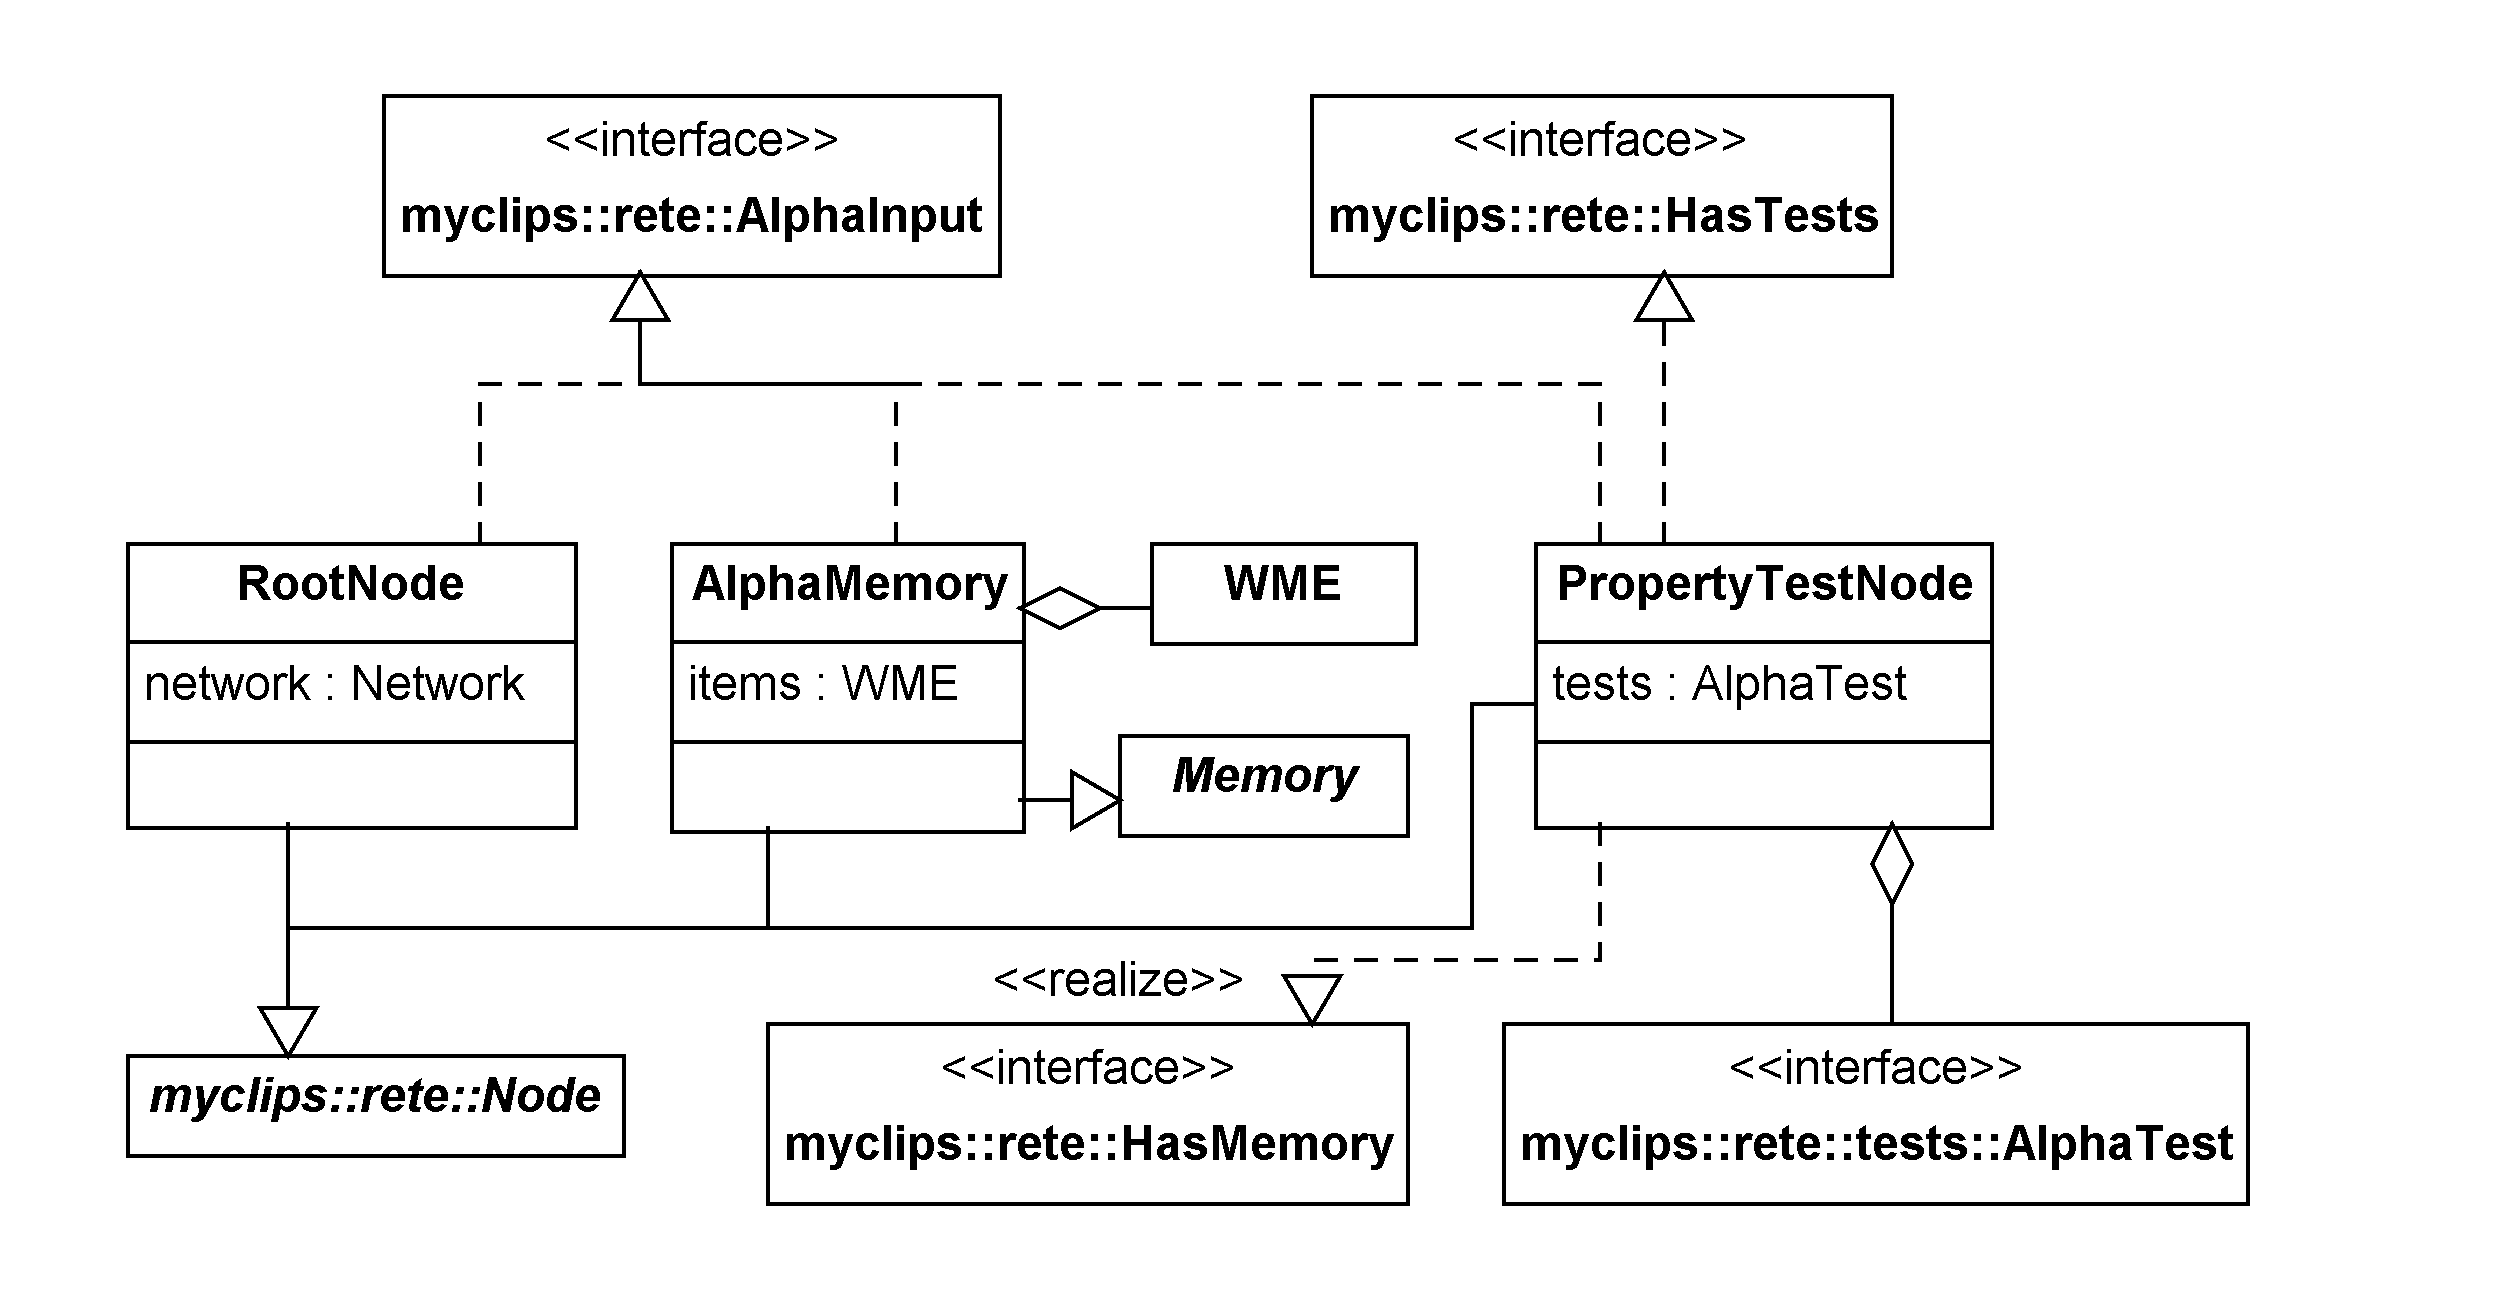
\includegraphics[width=1\textwidth]{Immagini/Capitolo3/Classi/myclips_rete_nodes_Nodi-Alpha.png}
\caption{Package \emph{myclips.rete.nodes}: vista dei nodi della pozione \emph{alpha}}\label{fig:class-myclips-rete-nodes-alpha}
\end{figure}

\begin{figure}
\centering
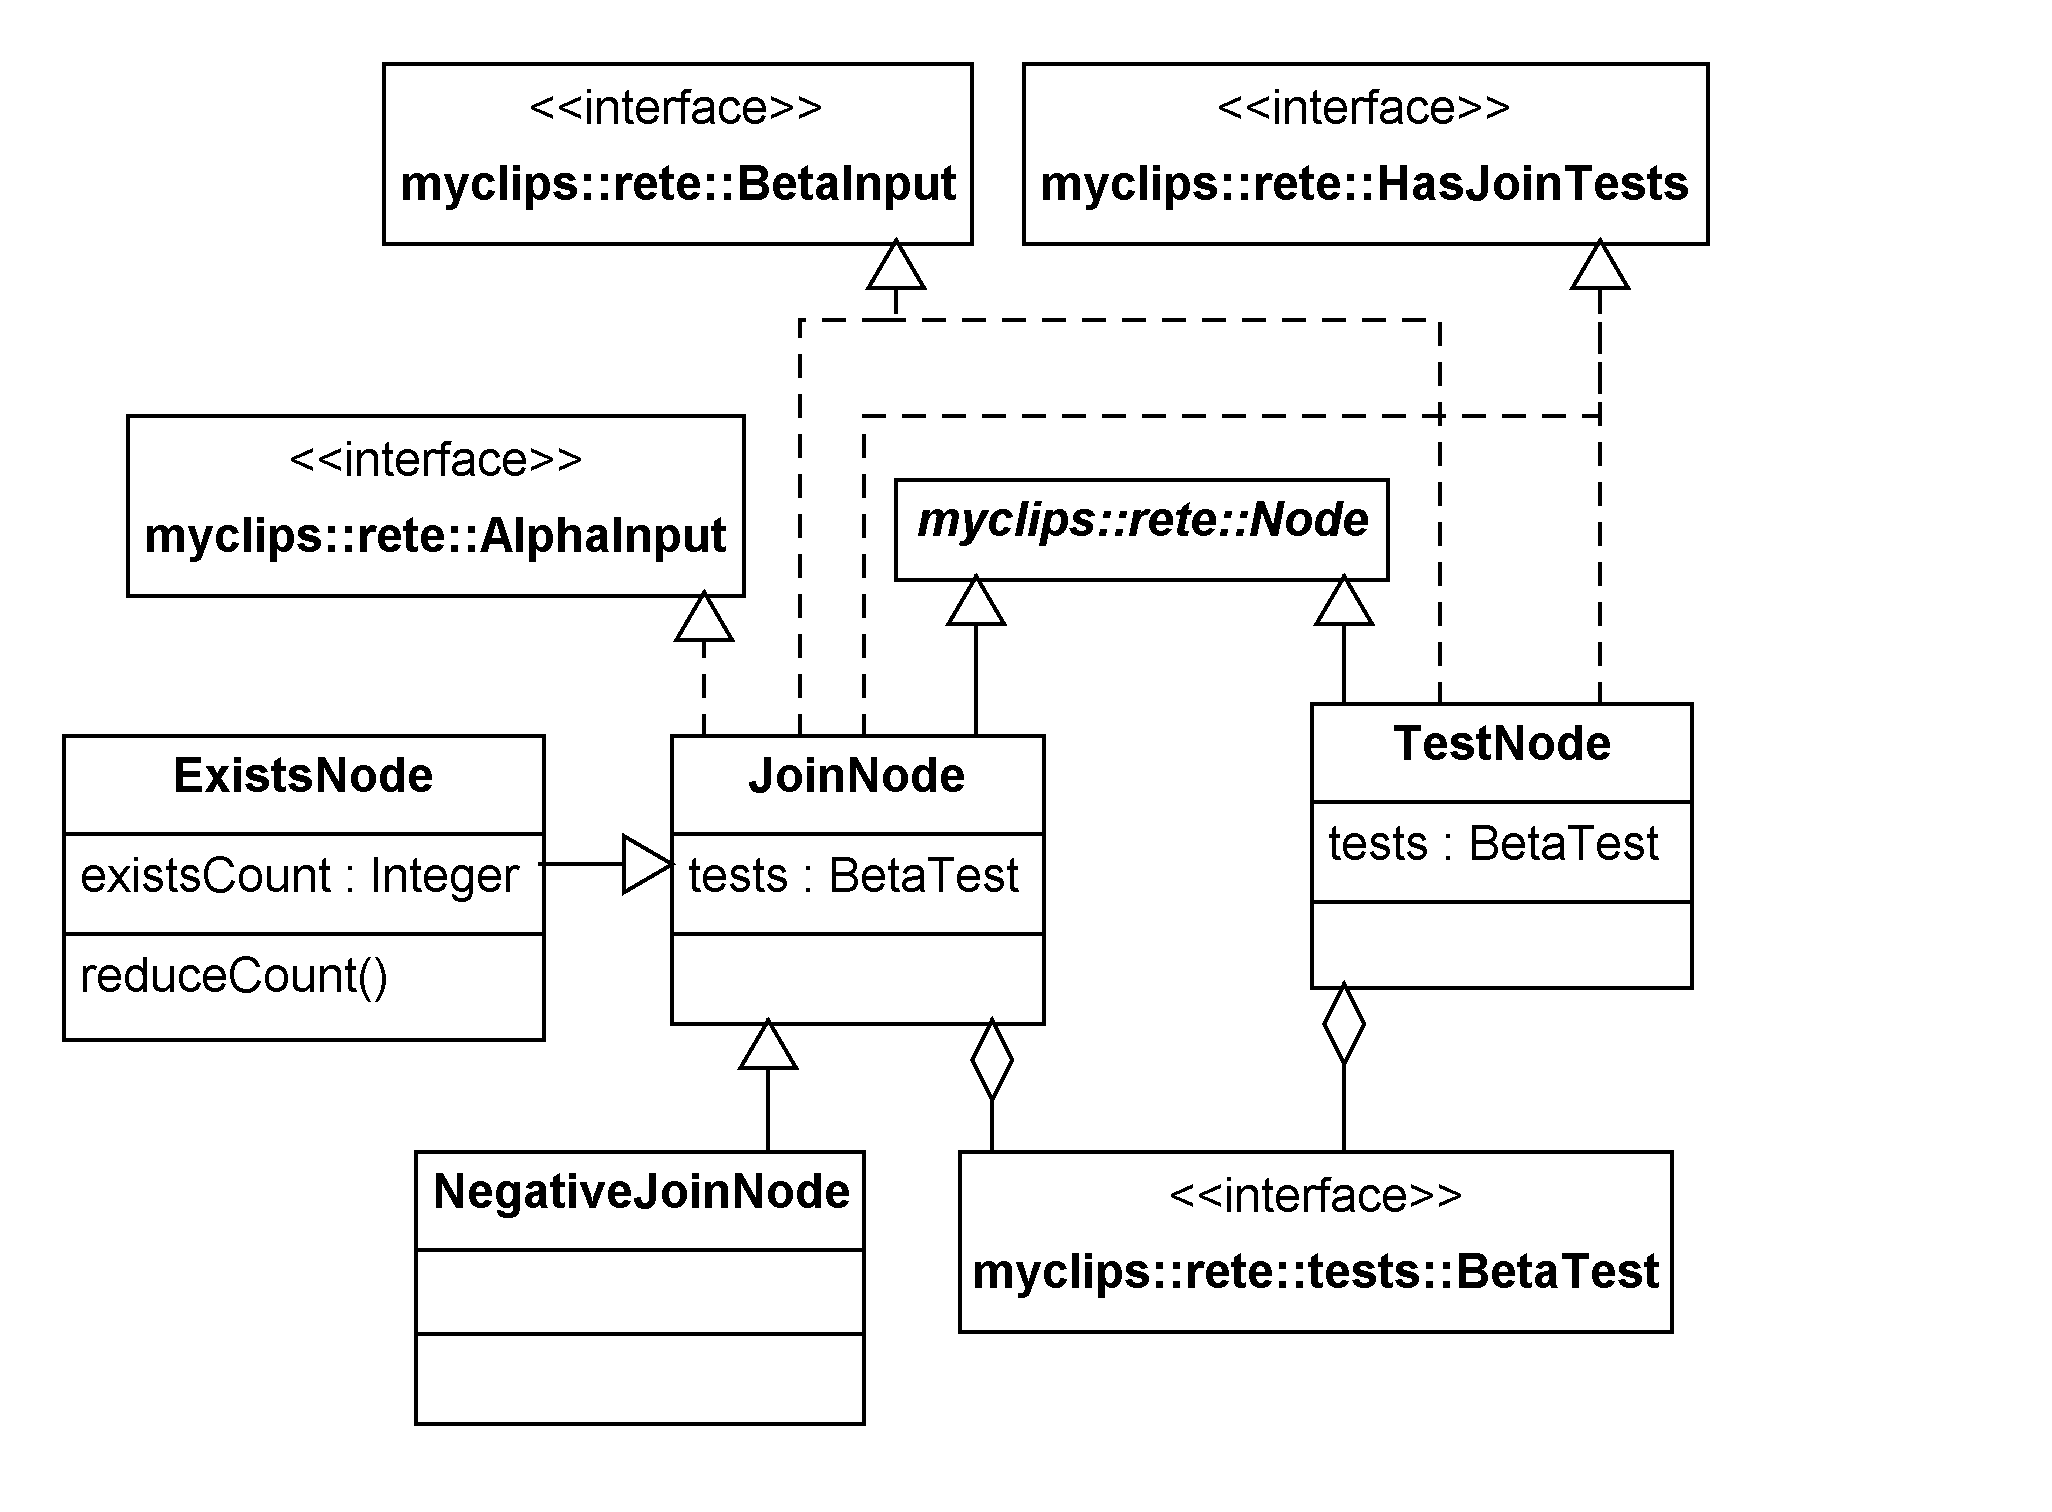
\includegraphics[width=1\textwidth]{Immagini/Capitolo3/Classi/myclips_rete_nodes_Join-Tests-Exists-Negative-Nodes.png}
\caption{Package \emph{myclips.rete.nodes}: vista dei nodi della pozione \emph{beta}}\label{fig:class-myclips-rete-nodes-beta}
\end{figure}

\begin{figure}
\centering
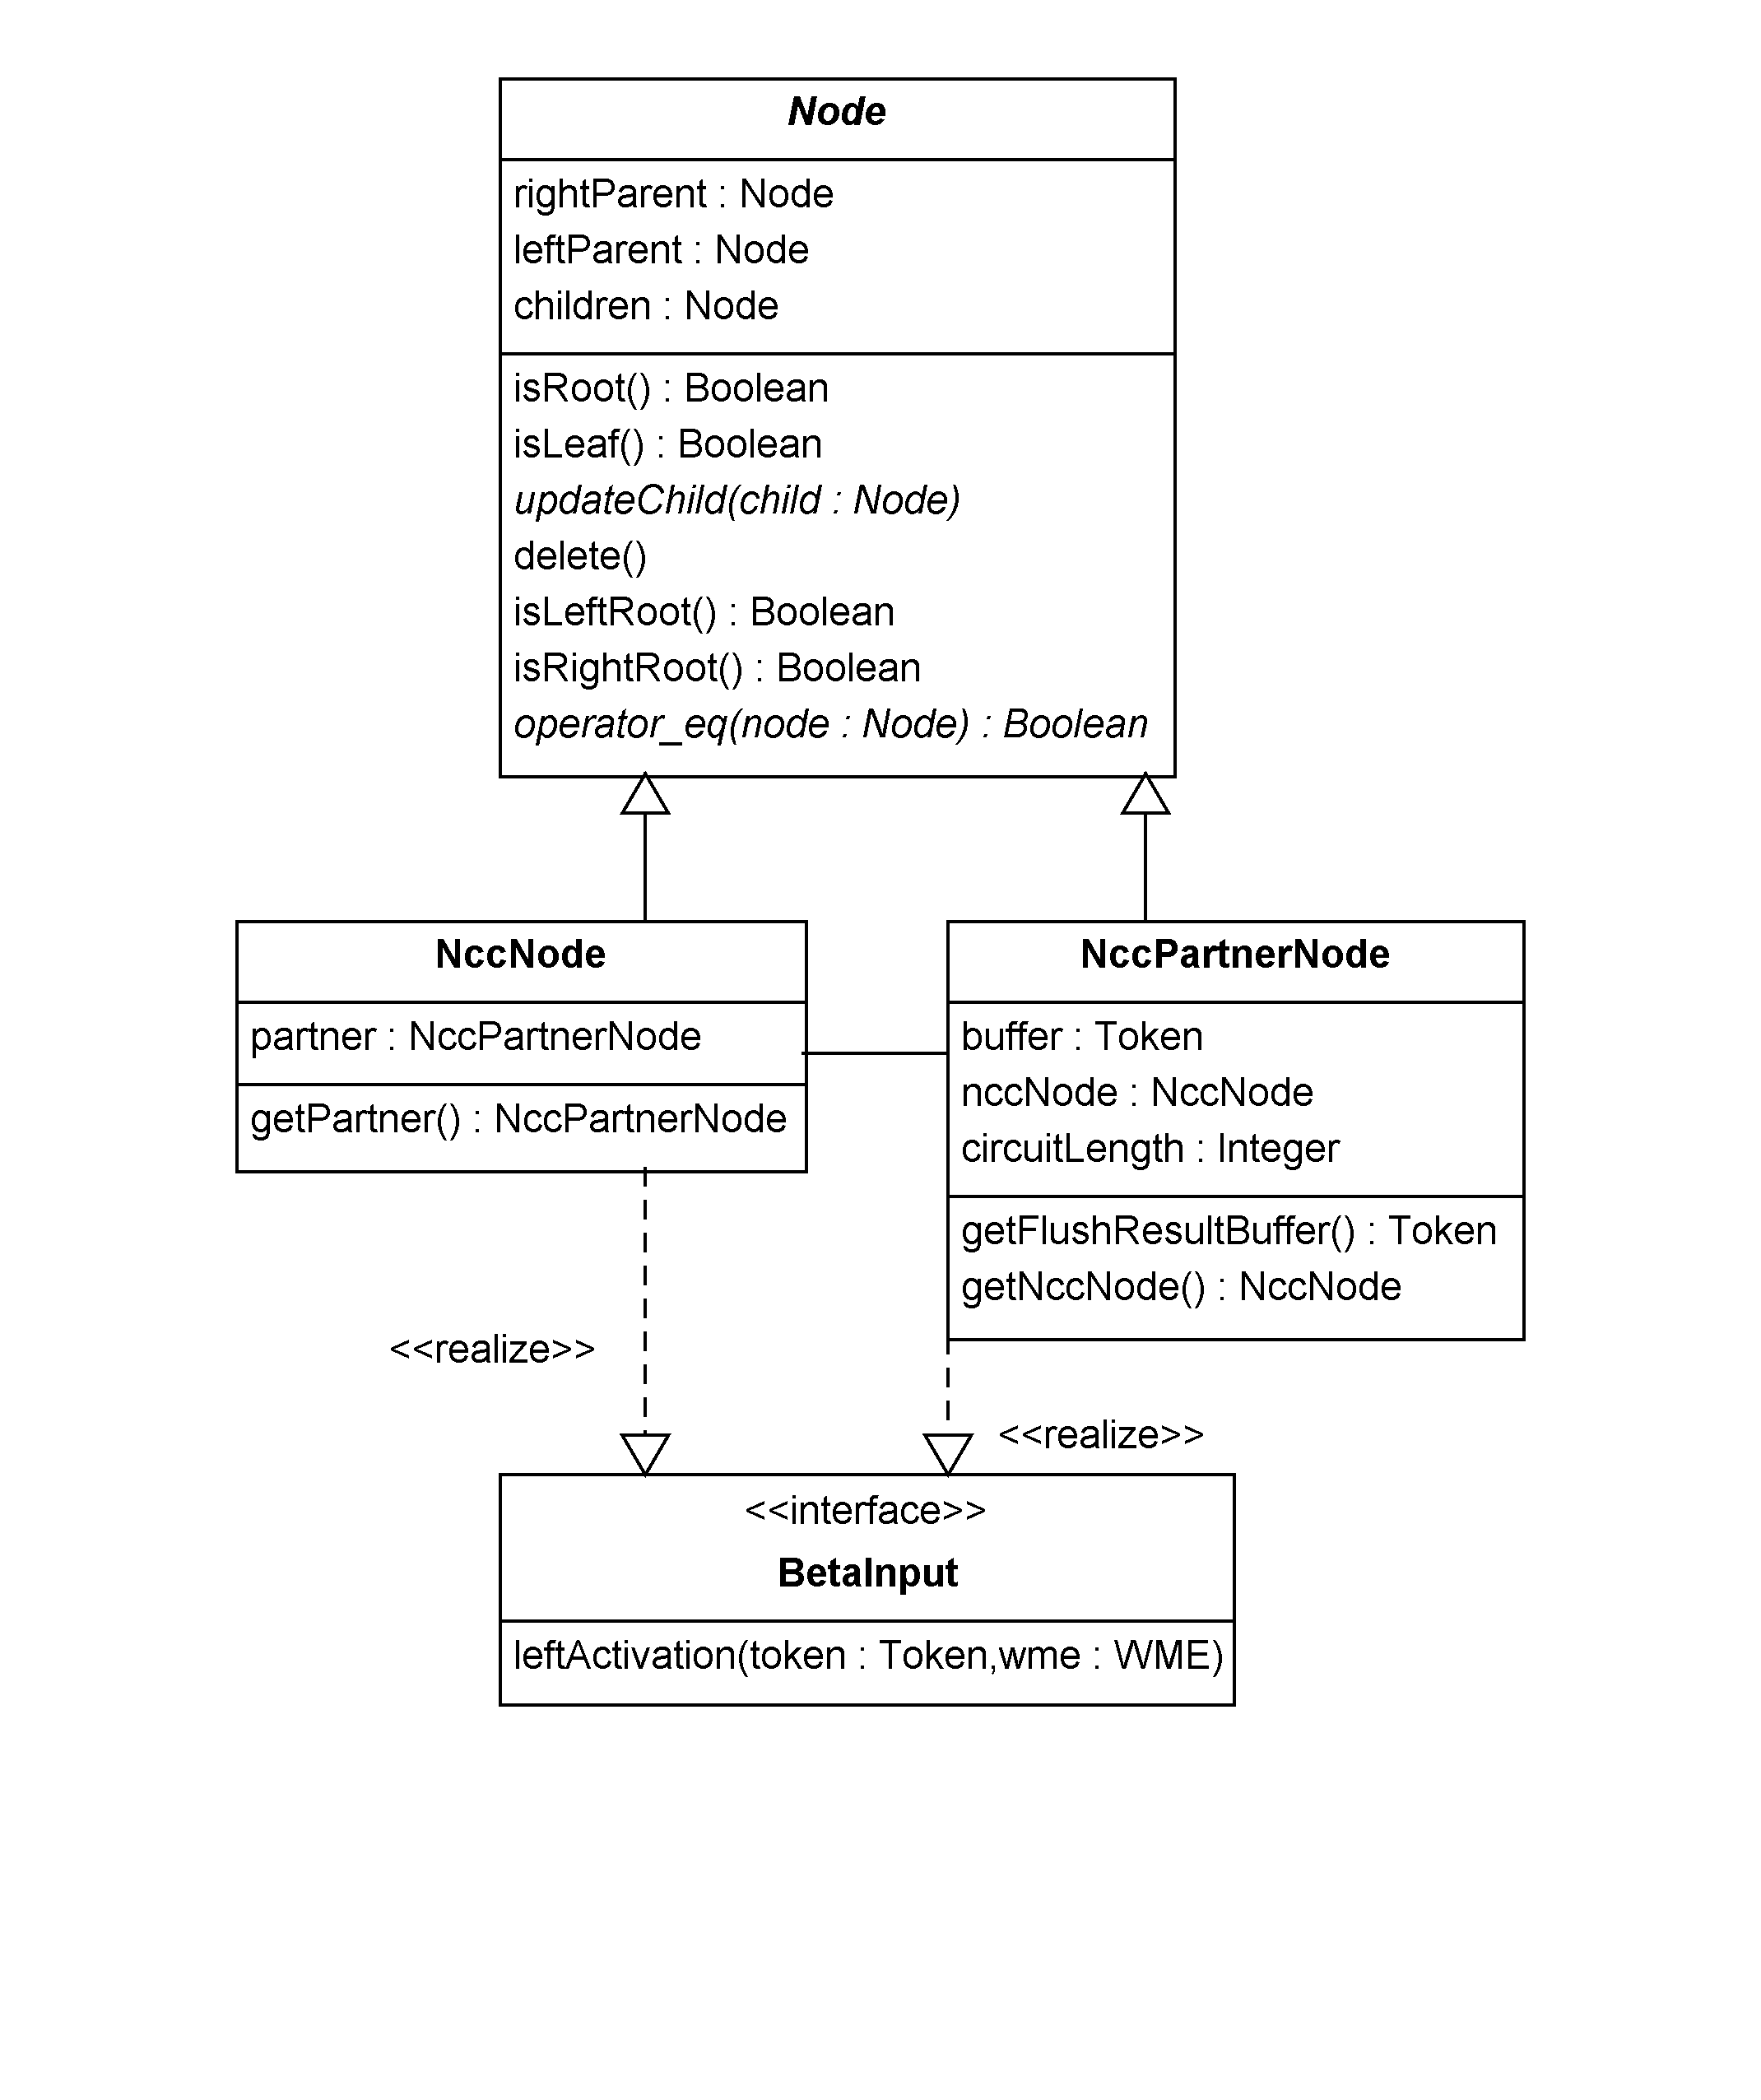
\includegraphics[width=1\textwidth]{Immagini/Capitolo3/Classi/myclips_rete_nodes_Ncc-Partner-Nodes.png}
\caption{Package \emph{myclips.rete.nodes}: vista dei nodi della pozione \emph{beta} (nodi \emph{Ncc})}\label{fig:class-myclips-rete-nodes-beta-ncc}
\end{figure}


Una classificazione approssimativa dei nodi può essere realizzata suddividendoli in base alla porzione della RETE che realizzano: \emph{alpha}~(\figurename~\ref{fig:class-myclips-rete-nodes-alpha}) o \emph{beta}~(\figurename~\ref{fig:class-myclips-rete-nodes-beta} e \ref{fig:class-myclips-rete-nodes-beta-ncc}). 

Ogni tipo di nodo svolge una specifica funzione, spesso anche in relazione alla tipologia di test che può inglobare:
\begin{description}
	\item[RootNode:] la radice del grafo radicato orientato che realizza RETE.
	
	\item[PropertyTestNode:] associabile a test di tipo \emph{alpha}, può effettuare controlli su elementi costanti di un pattern.
	
	\item[AlphaMemory:] unità locale di memoria posta a termine di ogni \emph{circuito alpha}. Conserva gli elementi \emph{WME} che hanno attraversato con successo il circuito a cui il nodo è collegato.
	
	\item[JoinNode:] nodo a due input, viene utilizzato per riunire istanze \emph{WME} provenienti dai due rami del grafo in \emph{Token} da propagare se i test collegati al nodo risultano verificati. Questo tipo di nodi viene utilizzato per realizzare i test di coerenza sul valore delle variabili presenti in pattern multipli.
	
	\item[NegativeJoinNode:] specializzazione del nodo \emph{JoinNode}, propaga un \emph{Token} solo se tutti i test di coerenza associati al nodo non risultano soddisfatti.
	
	\item[TestNode:] nodo con input singolo, esegue dei test su un \emph{Token} (spesso associati all'esecuzioni di funzioni dinamiche) e lo propaga nei casi di esito positivo.

	\item[ExistsNode:] nodo a due input utilizzato per fornire supporto al quantificatore esistenziale ($\exists$) all'interno delle porzioni LHS delle regole. Un'attivazione proveniente dal ramo sinistro (quindi \emph{beta}) del grafo viene propagato soltanto se esiste almeno un elemento all'interno dell'unità di memoria collegata come input destro (quindi \emph{alpha}).
	
	\item[NccNode] e \textbf{NccPartnerNode:} i nodi \emph{Ncc}~(\figurename~\ref{fig:class-myclips-rete-nodes-beta-ncc}) vengono utilizzati per realizzare negazioni di gruppi di condizioni. Le attivazioni provenienti dal ramo sinistro vengono propagate soltanto quando non viene identificata nessuna attivazione proveniente dal circuito negato associato.
	
\end{description} 

\paragraph{Classi di Test}

Gli algoritmi utilizzati dai nodi per eseguire le verifiche sulle attivazioni e gli elementi della \emph{working-memory} sono organizzati all'interno del \emph{package} \emph{myclips.rete.tests}. Alla base della strategia di progettazione dei test c'è l'utilizzo del \emph{design pattern} comportamentale \emph{Strategy}: allo scopo di rendere gli algoritmi di test intercambiabili fra loro, vengono fornite due interfacce di base che tutti i test realizzano. La scelta dell'interfaccia da implementare indica la classe di nodi che potranno utilizzare i test: \emph{AlphaTest} per i test utilizzabili nei nodi \emph{Alpha}, \emph{BetaTest} per quelli nei nodi \emph{Beta}.

\begin{figure}
\centering
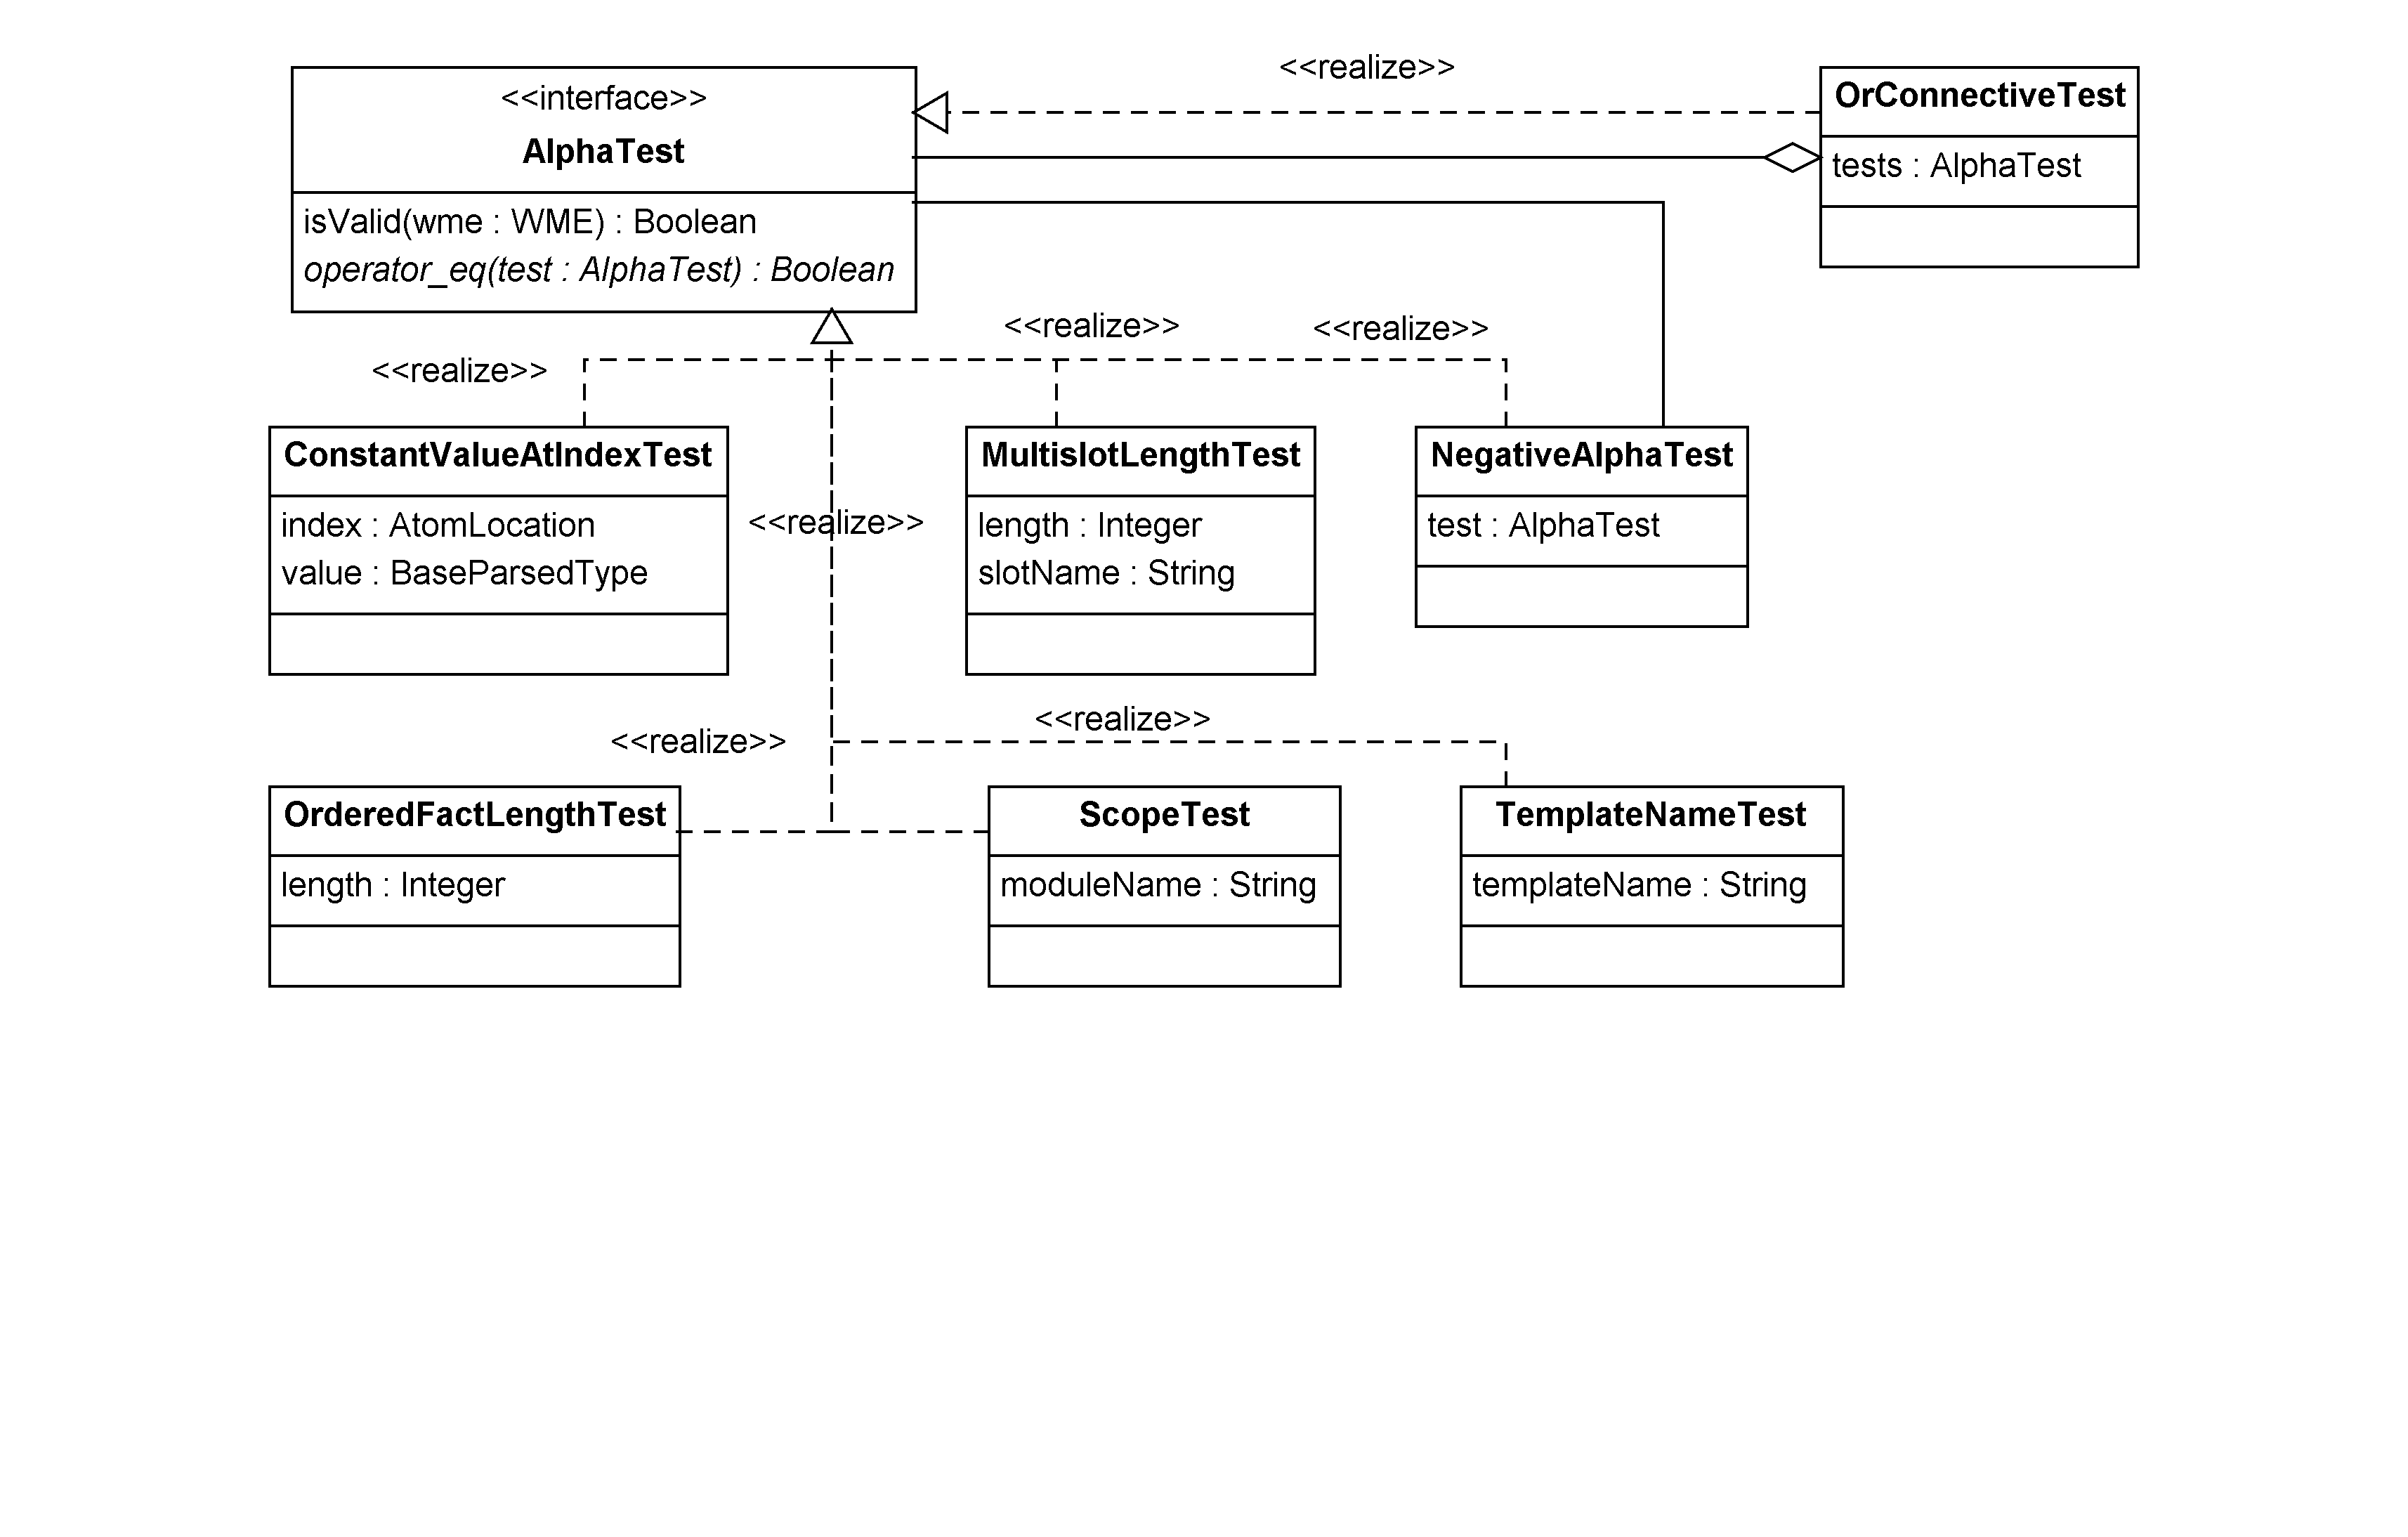
\includegraphics[width=1\textwidth]{Immagini/Capitolo3/Classi/myclips_rete_tests_Alpha.png}
\caption{Package \emph{myclips.rete.tests}: vista dei test eseguiti nella porzione \emph{alpha}}\label{fig:class-myclips-rete-tests-alpha}
\end{figure}

La prima tipologia (\figurename~\ref{fig:class-myclips-rete-tests-alpha}) esegue test su singoli elementi \emph{WME}, valutando il possibile inserimento all'interno delle memorie locali presenti al termine dei circuiti \emph{alpha}. Gli algoritmi possono valutare caratteristiche differenti dei singoli elementi come la lunghezza delle sequenze di \emph{OrderedFact}, la visibilità relativa ad un determinato \emph{Scope}, la presenza di un elemento costante in una determinata coordinata, etc.

\begin{figure}[h]
\centering
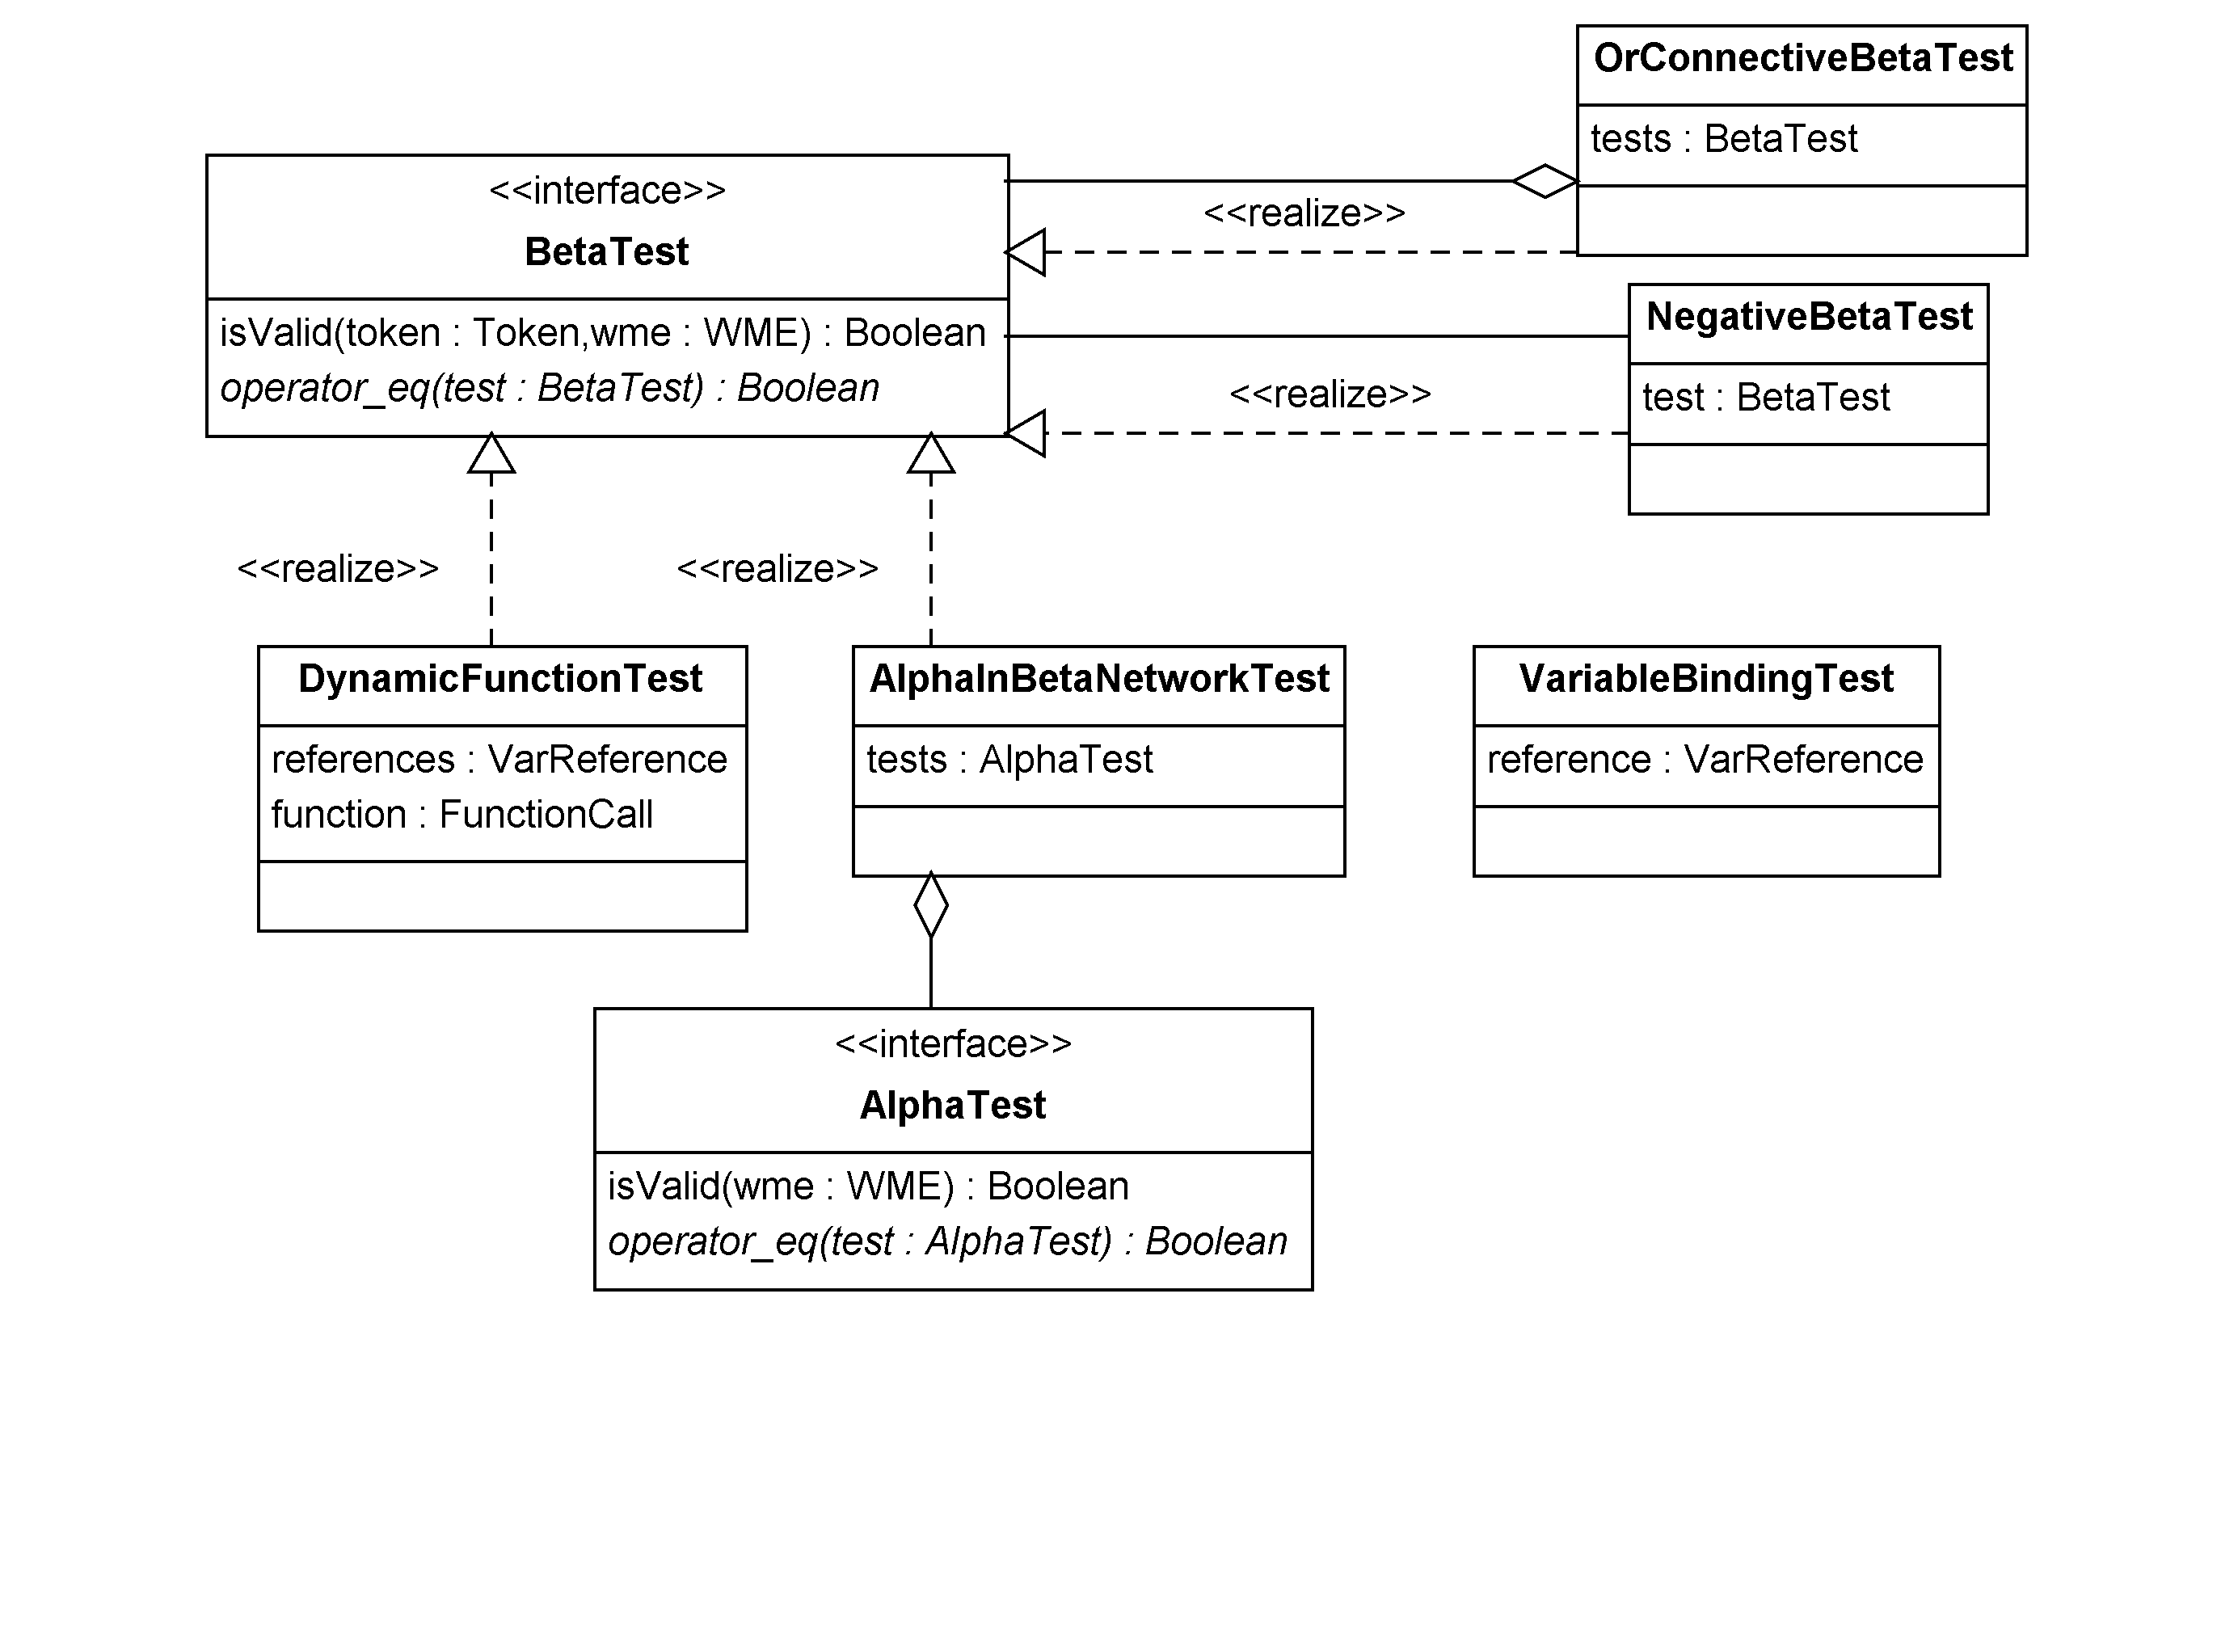
\includegraphics[width=1\textwidth]{Immagini/Capitolo3/Classi/myclips_rete_tests_Beta.png}
\caption{Package \emph{myclips.rete.tests}: vista dei test eseguiti nella porzione \emph{beta}}\label{fig:class-myclips-rete-tests-beta}
\end{figure}

La seconda tipologia (\figurename~\ref{fig:class-myclips-rete-tests-beta}) esegue verifiche su gruppi di \emph{WME}, rappresentati da \emph{Token}, valutando la coerenza del valore di variabili comuni a più pattern, il risultato dell'esecuzione di funzioni o valutando i risultato di test di tipo \emph{alpha} eseguiti nella porzione \emph{beta} del grafo. Al fine di poter eseguire i test di tipo \emph{alpha} nei nodi di tipo \emph{beta} è stata adottata una strategia facente riferimento al \emph{design pattern} strutturale \emph{Adapter} (anche noto con il nome di \emph{Wrapper} o \emph{Translator}): la classe \emph{AlphaInBetaNetworkTest}, che realizza l'interfaccia \emph{BetaTest}, incapsula oggetti con interfaccia \emph{AlphaTest} al suo interno. Le operazioni di traduzione degli argomenti dei test vengono eseguite all'interno dell'implementazione della classe.

\subsubsection{Modulo Interprete}

\begin{figure}[h]
\centering
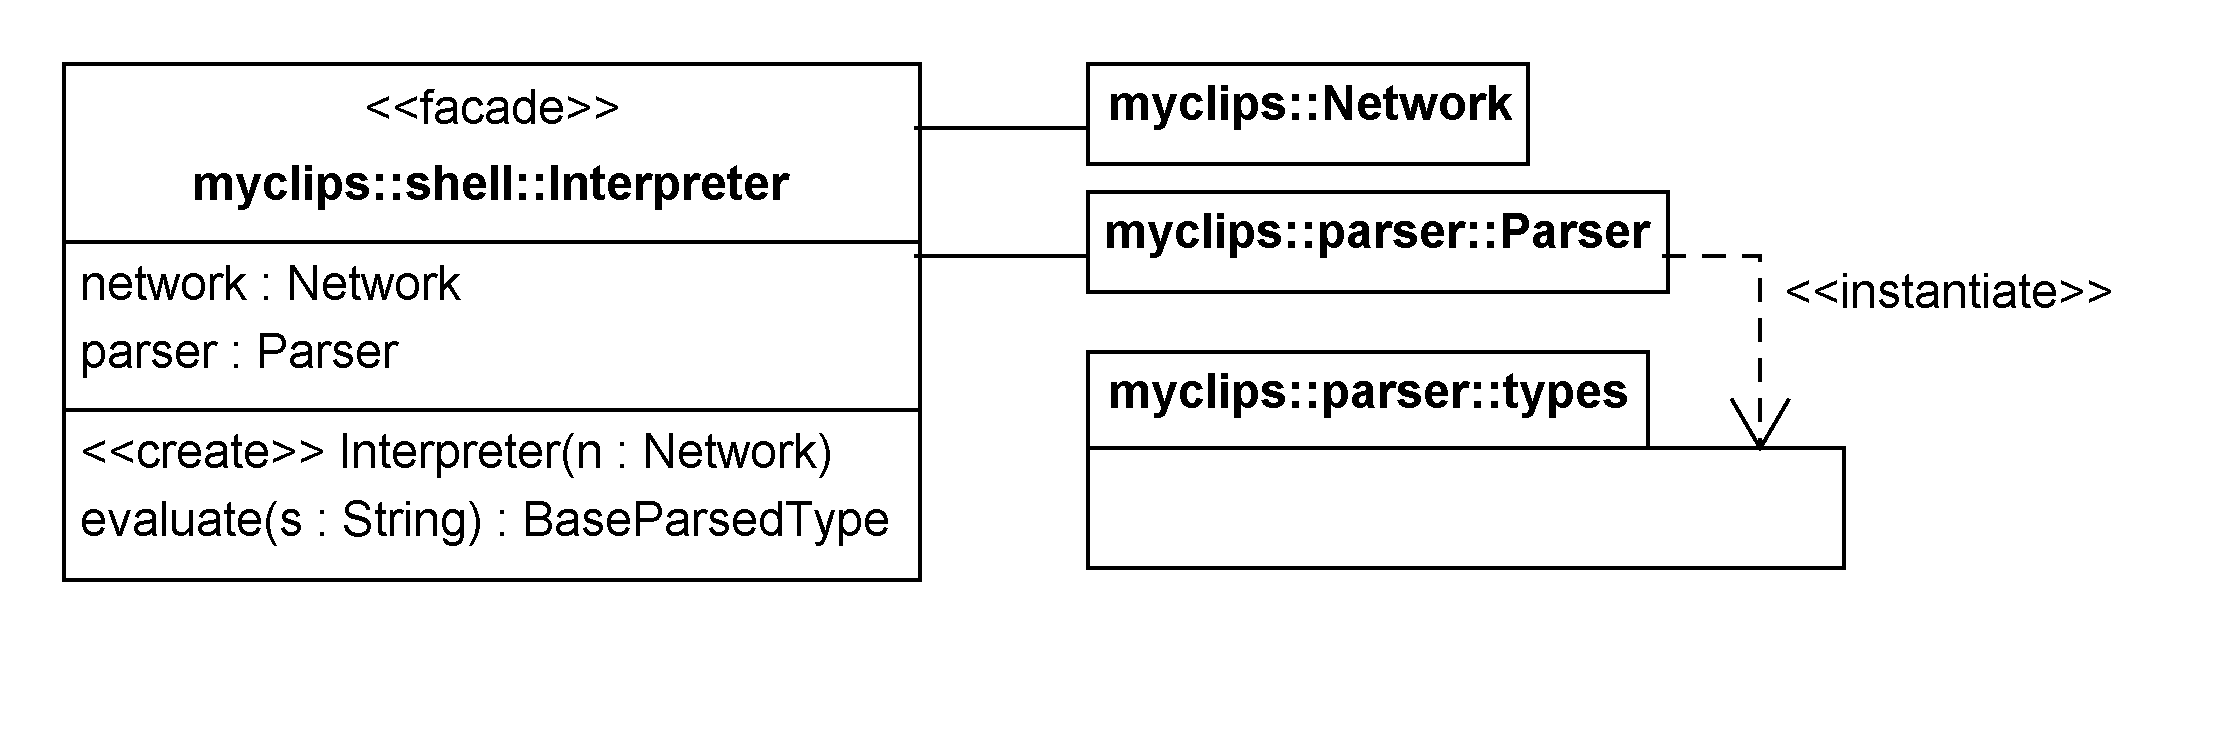
\includegraphics[width=1\textwidth]{Immagini/Capitolo3/Classi/myclips_shell_Interpreter.png}
\caption{Package \emph{myclips.rete.shell}: vista della classe \emph{Interpreter}}\label{fig:class-myclips-shell-interpreter}
\end{figure}

Il modulo \emph{Interprete}, contenuto nel \emph{package} \emph{myclips.shell}, consiste di un'unica classe \emph{fa\c{c}ade}: \emph{Interpreter}. Lo scopo della classe è quello semplificare ed unificare le operazioni di \emph{parsing} e valutazione dei costrutti, associandole alle attività di inizializzazione del \emph{motore inferenziale} e all'esecuzione del ciclo principale~(\figurename~\ref{fig:class-myclips-shell-interpreter}).

L'unica attività svolta dall'\emph{Interpreter} è quella di inizializzare un'istanza del \emph{Parser}, richiedere la valutazione di stringhe rappresentanti singoli \emph{costrutti} o \emph{comandi} e, se necessario, avviare l'interpretazione del costrutto dal parte di un'istanza di \emph{Network}. Nel caso l'elemento valutato dal parser sia un \emph{comando} (una chiamata a funzione di sistema), l'interprete provvede all'esecuzione dello stesso.

\subsubsection{Modulo Events Manager}

\subsubsection{Modulo Funzioni}

\subsection{Server}

\subsubsection{Broker di servizi}

\subsubsection{Servizio Sessioni}

\subsubsection{Servizio Registro tipi}

\subsubsection{Servizio Client IO}

\subsubsection{Servizio Client Events}

\subsubsection{Servizio Remote Shell}

\subsubsection{Servizio Engine}

\subsection{Terminale}

\section{Implementazione}

\subsection{Il linguaggio Python}

\subsection{Software utilizzato}


\section{Valutazione}

\subsection{Metriche}

\subsection{Correttezza}

\subsection{Prestazioni}


\section{Conclusioni}

\subsubsection{Sviluppi futuri}
